\documentclass[a4paper,11pt]{book}
%\documentclass[a4paper,11pt,twoside]{report}
\usepackage{etex}
\usepackage[english]{babel}
\usepackage{multicol}
\usepackage[T1]{fontenc}     %%%%%%%%%% Riga da togliere se si compila con PDFLaTeX
\usepackage[utf8]{inputenc} 
\frenchspacing 
\usepackage{graphicx}
\usepackage{textcomp}          
\usepackage{amsmath, amsfonts, amssymb}
\graphicspath{{./immagini/},{./Frontespizio/}}
\usepackage{float}
\usepackage{array}
\usepackage[makeroom]{cancel}
\title{}
\author{}
\date{}
\usepackage{tabularx}
\usepackage{bigstrut}
\setcounter{secnumdepth}{5}
\newcommand{\myparagraph}[1]{\paragraph{#1}\mbox{}\\}
\usepackage{caption}
\usepackage{subcaption}
\usepackage{bm}
\usepackage{pgfplots}
\usepackage{tikz}
\usepackage{tikz-cd}
\usetikzlibrary{cd}
\usetikzlibrary{arrows.new}
\usetikzlibrary{quotes}
%\usepackage{subfig}
\usepackage{./package/mcode}
%\usepackage[bw]{./package/mcode}
\usepackage{graphicx}
\usepackage{pdfpages}
\usepackage[figuresleft]{rotating}


\makeatletter
\tikzset{
  RL/.style={% without calc
    rounded corners={1pt},
    to path={% we asume that you use this path only on nodes (otherwise it will get tricky)
      \pgfextra
        \pgf@process{\pgfpointanchor{\tikztostart}{east}}%
        \pgf@xa\pgf@x\pgf@ya\pgf@y
        \pgf@process{\pgfpointanchor{\tikztotarget}{east}}%
        \pgf@xb\pgf@x\pgf@yb\pgf@y
        \ifdim\pgf@xb>\pgf@xa
          \pgf@xa\pgf@xb
        \fi
        \pgfmathsetlength\pgf@xc{#1}%
        \advance\pgf@xa\pgf@xc
      \endpgfextra
      -- (+\pgf@xa,+\pgf@ya) -- (+\pgf@xa,+\pgf@yb) \tikztonodes -- (\tikztotarget)
    }
  },
  RL/.default=0.7cm}


\tikzset{
  LL/.style={% without calc
    rounded corners={1pt},
    to path={% we asume that you use this path only on nodes (otherwise it will get tricky)
      \pgfextra
        \pgf@process{\pgfpointanchor{\tikztostart}{west}}%
        \pgf@xa\pgf@x\pgf@ya\pgf@y
        \pgf@process{\pgfpointanchor{\tikztotarget}{west}}%
        \pgf@xb\pgf@x\pgf@yb\pgf@y
        \ifdim\pgf@xb>\pgf@xa
          \pgf@xa\pgf@xb
        \fi
        \pgfmathsetlength\pgf@xc{#1}%
        \advance\pgf@xa\pgf@xc
      \endpgfextra
      -- (+\pgf@xa,+\pgf@ya) -- (+\pgf@xa,+\pgf@yb) \tikztonodes -- (\tikztotarget)
    }
  },
  LL/.default=-5cm}

\usepackage{booktabs}
\newsavebox\ltmcbox

\usepackage{enumerate}
\usepackage{longtable}
\usepackage{footnote}

%\usepackage{float}
\usepackage{multirow}
\usepackage{enumitem}
%\setlist{nolistsep}
\pgfplotsset{compat=1.3}


%\usepackage[top=1.2in, bottom=0.8in, left=1.2in, right=0.8in]{geometry}
\usepackage[top=3.5cm, bottom=2.5cm, left=4cm, right=2.5cm]{geometry}

%\usepackage[all]{xy}

\usepackage[ocgcolorlinks,hidelinks]{hyperref}
\usepackage{xcolor}
% for coloured links
%\hypersetup{
%    colorlinks,
%    linkcolor={red!0!black},
%    citecolor={blue!50!black},
%    urlcolor={blue!80!black}
%}

% for printing compile with this
\hypersetup{
    colorlinks,
    linkcolor={red!0!black},
    citecolor={blue!0!black},
    urlcolor={blue!0!black}
}



\usepackage{./package/structuralanalysis}

% frontespizio
\usepackage[]{lmodern}
\usepackage[]{microtype}
\usepackage {lettrine}
\usepackage {epigraph}
\usepackage {url}
\usepackage {mathrsfs}
\usepackage {sidecap}	      
\usepackage {caption}
\usepackage{lmodern}
\usepackage{booktabs}    



% draw lines for legend in caption
\def\drwln#1#2{\raise 2.5pt\vbox{\hrule width #1pt height #2pt}}
\def\solid{\drwln{24}{1.0}\ }
\def\spc#1{\hskip #1pt}
\def\dashed{\hbox {\drwln{4}{1.0}\spc{2}
                   \drwln{4}{1.0}\spc{2}\drwln{4}{1.0}}\nobreak\ }
\def\dashdot{\hbox {\drwln{8}{1.0}\spc{2}
                   \drwln{2}{1.0}\spc{2}\drwln{8}{1.0}}\nobreak\ }
\def\dotted{\hbox {\drwln{1}{1.0}\spc{2}
                   \drwln{1}{1.0}\spc{2}\drwln{1}{1.0}}\nobreak\ }
\def\ldash{\hbox {\drwln{8}{1.0}\spc{2}
                  \drwln{8}{1.0}\spc{2}\drwln{8}{1.0}}\nobreak\ } 
\def\dashcirc{\hbox {\drwln{8}{1.0}\spc{2}
                   $\circ$\spc{2}\drwln{8}{1.0}}\nobreak\ }   
\def\dashsqr{\hbox {\drwln{8}{1.0}\spc{2}
                   $\square$\spc{2}\drwln{8}{1.0}}\nobreak\ }              
\def\colrule{\\[-7.5pt]\hline\\[-5pt]}
\def\botrule{\\[-7.7pt]\hline}
\def\dashrule{\\[-7.5pt]\dashed\\[-5pt]}
 


\newcommand{\de}{\partial}
\newcommand{\Nabla}{\bar\nabla}
\newcommand{\curl}{\nabla\times}
\renewcommand{\Re}{\textnormal{Re}}
\newcommand{\Pe}{\textnormal{Pe}}
\newcommand{\Ch}{\textnormal{Ch}}
\newcommand{\Fr}{\textnormal{Fr}}
\newcommand{\We}{\textnormal{We}}

\DeclareRobustCommand{\univsc}[1]{\Large\textsc{\textls[75]{#1}}}
\DeclareRobustCommand{\titlesc}[1]{\linespread{1.2}\LARGE{\textls[50]{\uppercase{#1}}\linespread{1}}}
\DeclareRobustCommand{\subtitlesc}[1]{\Large\textsc{\textls[50]{#1}}}
\DeclareRobustCommand{\namesc}[1]{\large\textsc{\textls[35]{#1}}} 

\usepackage[bordercolor=black,linecolor=black,backgroundcolor=white,textwidth=3.5cm]{todonotes}
\reversemarginpar

\usepackage[round]{natbib}
\usepackage{commath}
 

\title{}
\author{Giovanni Soligo \& Alessio Roccon}
\date{\today}
%%%%%%%%%%%%%%%%%%%%%%%%%%%%%%%%%%%%%%%%%%%
\begin{document}

\begin{titlepage}

\tikz[remember picture,overlay] \node[opacity=0.8,inner sep=0pt] at (current page.center){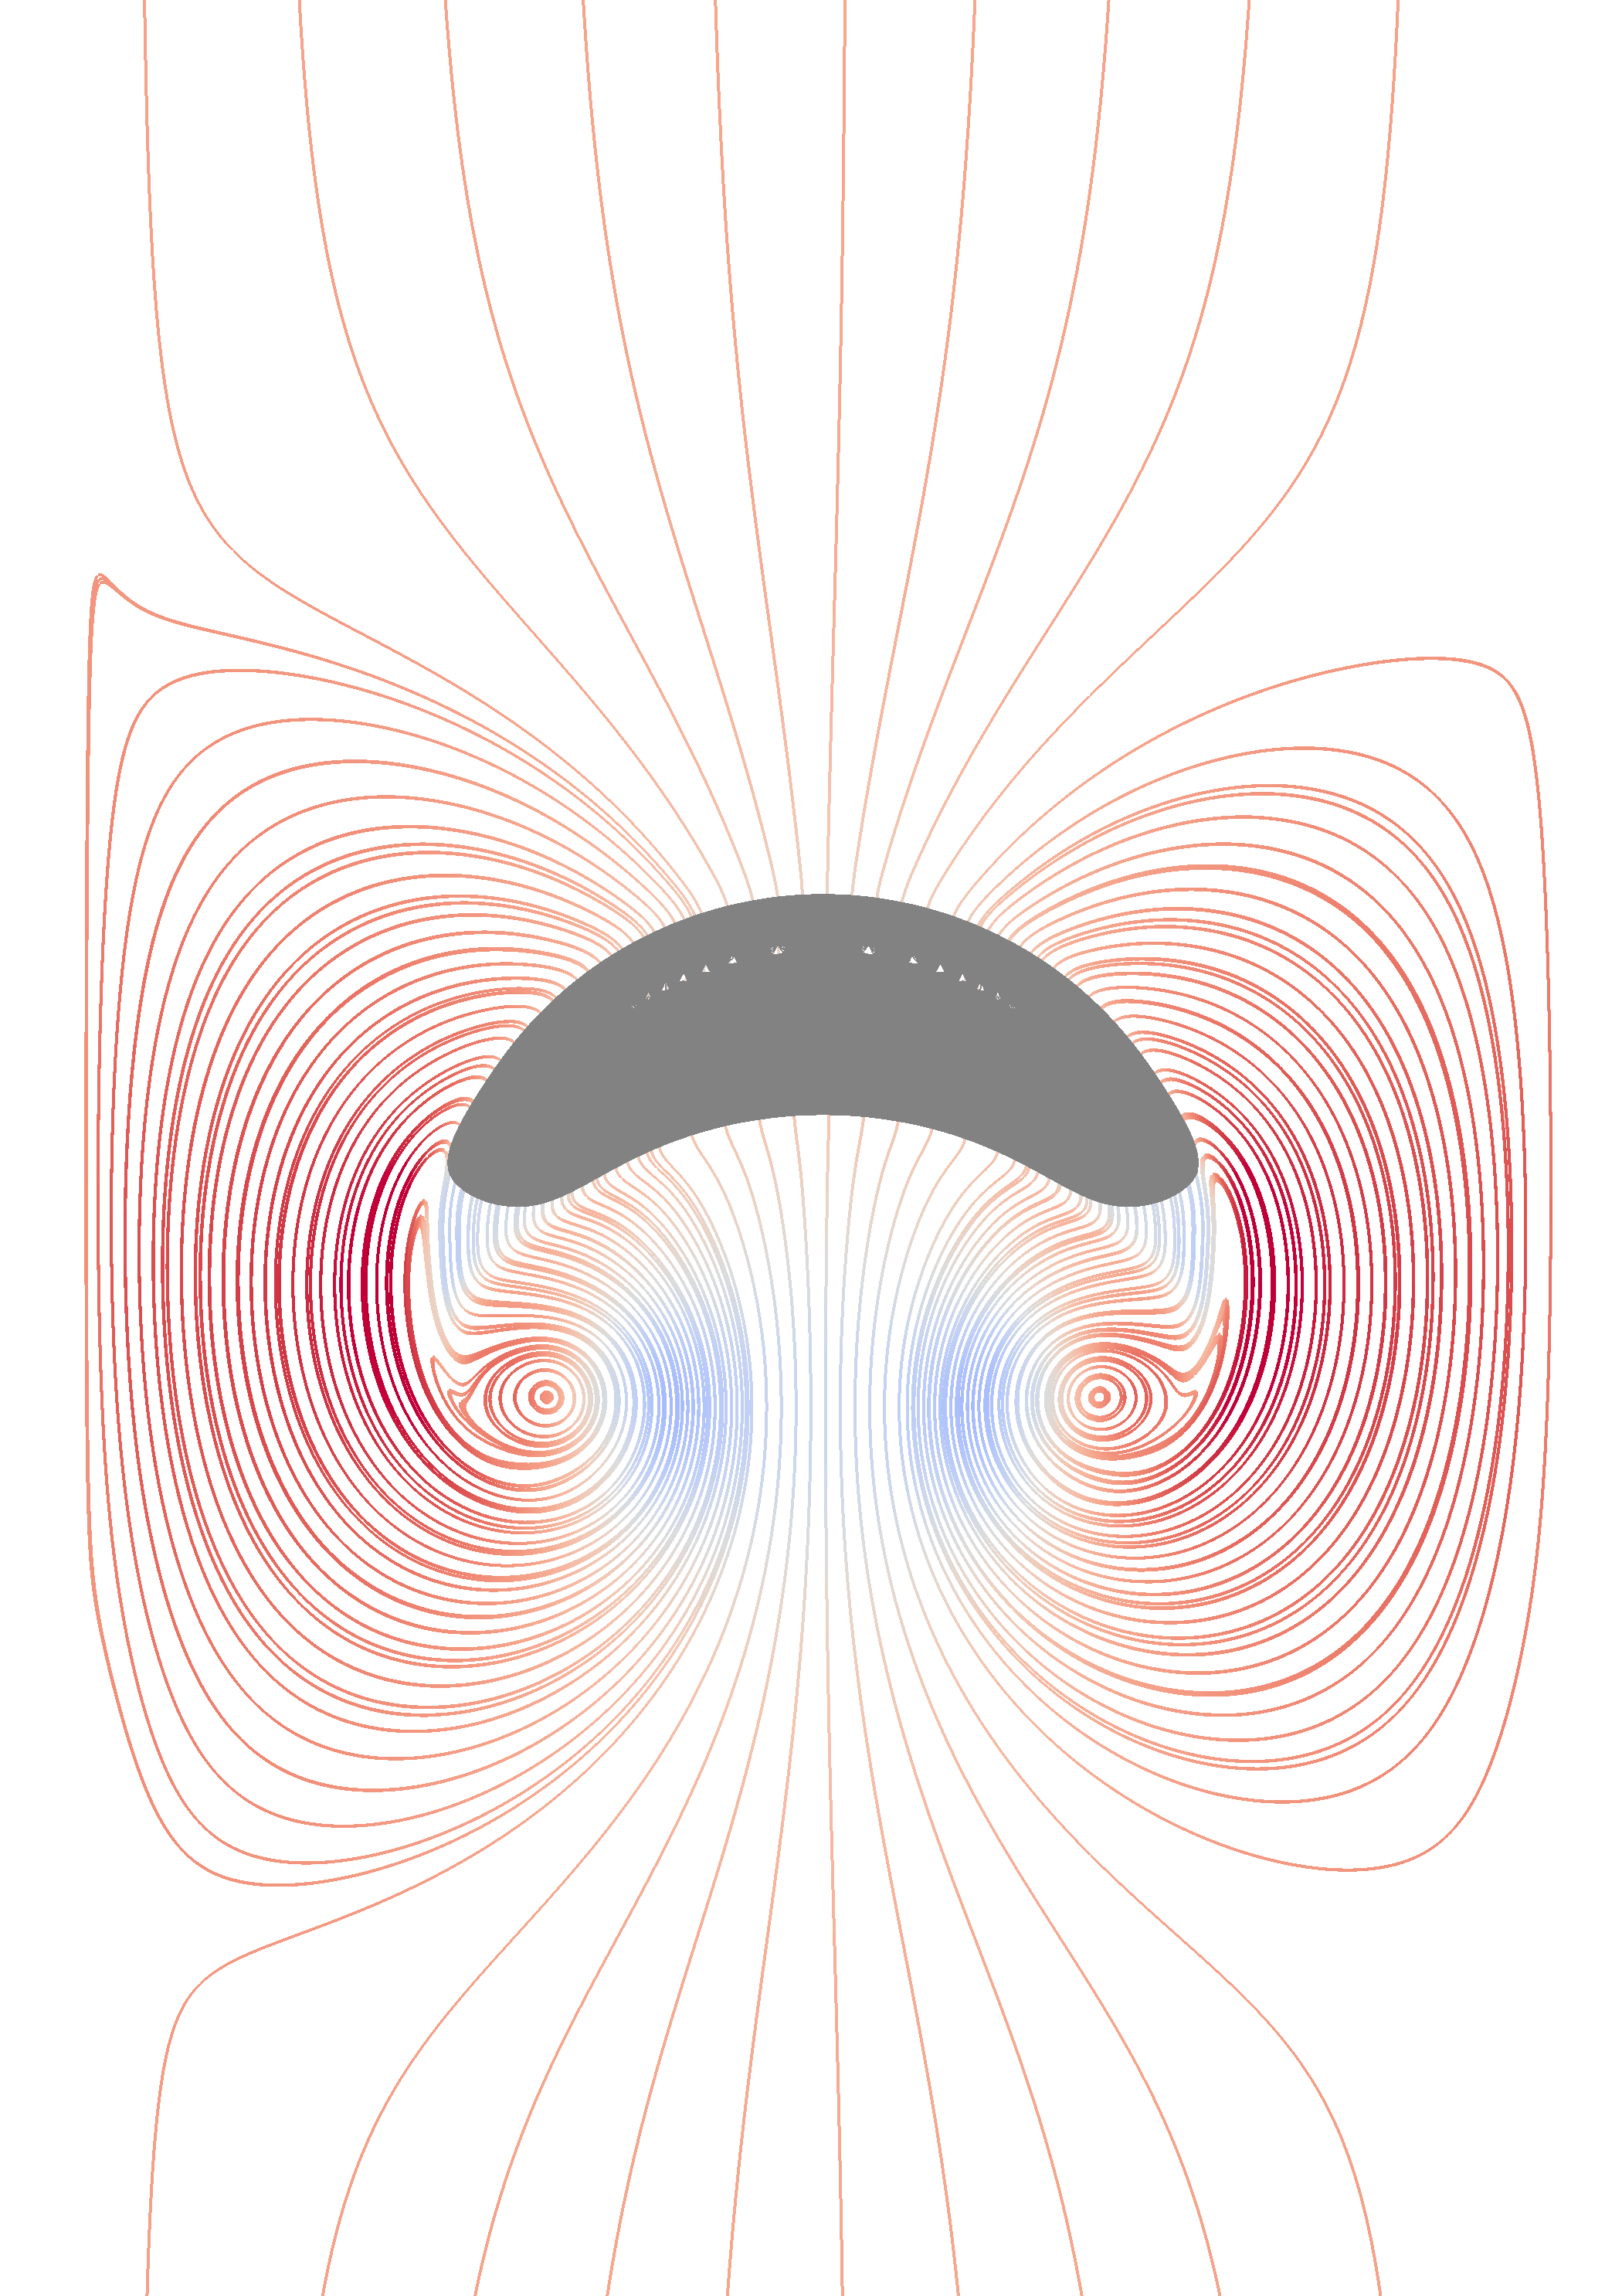
\includegraphics[width=\paperwidth,height=\paperheight]{bubble2}};


  \begin{center}  
\medskip   
  \rule{14cm}{1pt}\\
  \medskip
  \vspace{\stretch{0.25}}
  \titlesc{\huge{\bfseries{FLOW36 Handbook}}} \\    [2ex]
  \subtitlesc{A complete guide to FLOW36} 
\vfill
 \vspace{-5cm}
\@author\\
\@date
 \vspace{5cm}
 \medskip   
  \rule{14cm}{1pt}\\
  
% 
%  \large
%  \begin{tabular*}{\textwidth}{@{}l@{\extracolsep{\fill}}r@{}}
%    \large Relatore:&Laureando:\\	
%     Prof.\ \namesc{Alfredo Soldati}  &\namesc{Giovanni Soligo}\\[0.3cm]	 %[1.3cm]
%     Prof.\ \namesc{Ugo Piomelli}  &   \\
%  \end{tabular*}
\end{center}

\end{titlepage}
\clearpage{\pagestyle{empty}\cleardoublepage}

\frontmatter
\setcounter{page}{1}
\date{\today}
This handbook is intended to give a general, but very detailed description of the code \texttt{FLOW36DUAL}.
The code was initially written in 2017 at TU Wien by \@author, as a replacement for the legacy code \texttt{FLOWSB}, in order to get better overall performance, a more readable and up to date code and improve its scalability.
The code was then ported to GPU architectures during the summer 2022.
The code performs Direct Numerical Simulations (DNS) in a channel geometry, using a pseudo-spectral spatial discretization. 
The flow solver is coupled with a phase variable solver, which solves the Cahn--Hilliard equation (phase-field method).
The solver can also accounts for the presence of surfactants (in the phase-field method framework) as well as describe a passive scalar (heat/mass transfer problems).
%The code was further developed during the MSCA-ITN-EID project COMETE "Next-Generation Computational Methods for Enhanced Multiphase Flow Processes” (No 813948) to simulate turbulent three-phase flows and turbulent bubbly-laden flows.


\vfill
\rule{14cm}{0.4pt}\\

This document was last updated on \@date.

\tableofcontents

\mainmatter
\chapter{Getting started}
The executable \texttt{compile.sh} includes all the parameters needed to run a simulation. In Section \ref{sec: compile} is reported a detailed guide about this file, its structure and how to modify it.\\
When running the \texttt{compile.sh} in its own folder, it sets up all the files and folders needed for the simulation in the \texttt{set\_run} folder.
Once the \texttt{compile.sh} has finished without error, go to the \texttt{set\_run} folder and launch the executable \texttt{go.sh}; at this point the simulation should start.\\
The main folder of the code includes the following files and subfolders:
\begin{itemize}
\item \texttt{initial\_fields} : contains the initial fields (velocity and phase, if dealing with a multiphase simulation) used if the initial condition is set to read the initial fields (both in its serial or parallel version). These files, during the execution of \texttt{compile.sh}, are copied into the \texttt{set\_run/initial\_fields} folder, so they can be removed or modified even when the simulation is running.
\item \texttt{Machine XYZ} : contains the \texttt{makefile} and \textit{go.sh} needed when running on the above mentioned machine. It is copied in the main folder by the \texttt{compile.sh} script when needed.
For some machines, more than one makefile (i.e. configuration) might be available depending on the compiler/libraries available and architecture (CPU, GPU).
Depending on the machine, also the \texttt{openacc\_flag} is set. 
This flag enables the GPU acceleration on the supported machines (e.g. Nvidia GPUs).
\item \texttt{paraview\_output} : contains the code that can be used to generate Paraview compatible output file (using a rectilinear grid).
\item \texttt{set\_run} : contains all the files and subfolders needed for a simulation and its output.
\item \texttt{source\_code} : contains all the subroutine and the main file used to compile the executable file; each subroutine will be described in detail in Chapter \ref{chap: flowchart}.
\item \texttt{stats\_calc} : contains the code that can be used to extract velocity statistics from the simulation output files (mean, root mean square, skewness and flatness). These statistics can also be calculated runtime as will be seen in Section \ref{sec: compile}.
%\item \texttt{VSC-3} : contains the \texttt{makefile} needed when running on VSC-3. It is copied in the main folder by the \texttt{compile.sh} script when needed.
\item \texttt{compile.sh} : this file is used to generate the simulation folder and executable. It also includes all the parameter declaration part.
\item \texttt{go.sh} : its edited version is copied during \texttt{compile.sh} execution in the \texttt{set\_run} folder and used to launch the simulation (directly on local machines or to be submitted to the job/load manager via batch commands).
\item \texttt{input.f90} : its edited version is copied during \texttt{compile.sh} execution in the \texttt{set\_run/sc\_compiled} folder and it is used as an input file for the simulation parameters.
\item \texttt{makefile} : called during \texttt{compile.sh} execution to create the executable of the code.
\item \texttt{scaling} : contains strong and weak scaling results obtained on different machines.
\item \texttt{profiling} : contains the profiling data obtained on Marconi-100 using GPU. The file can be view using Nvidia Nsight Systems.
\end{itemize}
On a local machine the code can be compiled and run just by executing the \texttt{compile.sh} script. On a cluster, since there is always a job scheduler that handles all the submitted jobs the last lines of the \texttt{compile.sh} script must be commented out (especially the call to the script \texttt{go.sh}). When running on a cluster, first run the \texttt{compile.sh} script, then move to the \texttt{set\_run} directory and submit the jobscript \texttt{go.sh}. If you want to compile and run several simulation with different parameters, after the compilation, copy the folder \texttt{set\_run} somewhere else and then submit the jobscribt to the job scheduler there.\\

\section{Output of a simulation}
Depending on the parameters choice when compiling the code, the code can give as an output different data, that will be all saved in the subfolder \texttt{results} inside the \texttt{set\_run} folder.\\
The code will always save the initial and final velocity fields (and the phase field, if it is activated) both in physical and modal space, the $x$, $y$, $z$ axis arrays and a time check file. This latter file will include the simulation current time, the bulk Reynolds number and, for the phase field case only, also the mean value of $\phi$ all over the domain and the integral of the phase $\phi=+1$ (to check the mass losses).\\
In addition the output of the simulation includes:
\begin{itemize}
\item Flow field data (and phase field, if activated) in physical space: \texttt{[variable name]\_[number of time step].dat}
\item Flow field data (and phase field, if activated) in modal space: \texttt{[variable name]c\_[number of time step].dat}
\item Mean, root mean square, skewness and flatness for the flow field ($u$, $v$, $w$) (single array in the wall-normal direction). Single formatted file \texttt{stats.dat}.
\item Mean pressure and root mean square of pressure fluctuations (single array in the wall-normal direction). The mean pressure value does not include the mean pressure gradient in $x$ and $y$ directions. The pressure solver works for a fully-developed channel flow with a non-zero mean velocity in the $x$ direction and for a single phase flow. Single formatted file \texttt{budget.dat}; the first lines of the file explain its content.
\item Energy budgets. For the pressure--strain correlation the pressure calculated above is used, so they do not consider the presence of multiple phases (the energy balance may not be zero for a multiphase flow, since some terms are missing/not properly calculated). The energy budgets are saved in the same file as the pressure (\texttt{budget.dat}).
\item Streamwise and spanwise power spectra for $u'$, $v'$ and $w'$ at $z^+=5$, $z^+=15$ and $z^+=\Re$. Power spectra in $x$ direction are saved in the file \texttt{power\_xspectra.dat}, while those in $y$ direction in the file \texttt{power\_yspectra.dat}.
\end{itemize}
Velocity and eventually phase field are saved in a binary file, written with the same endianness and format as the MPI implementation of the machine where the simulation was run.\\
In future others output may be added to the code.

\section{Post-processing}
At the present time two codes are available for direct post-processing of the output data; the first one, in the folder \texttt{stats\_calc} evaluate the statistics of the flow field (can be done also at run-time), while the other, \texttt{paraview\_output\_fg}, generates Paraview compatible output file. Both these codes use either data in physical space, either in modal space.\\
The statistics calculation runs alway on three MPI processes, one handle $u$ data, another $v$ data and the third $w$ data. The Paraview output generation can work independently on several cores: each core takes care of writing the output at a certain time-step. Use the input file to modify some parameters of the program to better handle the output.

\section{The \texttt{compile.sh} file}
\label{sec: compile}
The script \texttt{compile.sh} is divided in several parts: input parameters declaration, cleaning of \texttt{set\_run} folder, copying and editing files in the \texttt{set\_run} folder, compilation of the code and, only on a local machine, running the \texttt{go.sh} in the proper folder.

\subsection{Parameters declaration}
When running a simulation this is the only part that should be modified; unless needed (e.g. code modification, \dots) all the rest of the script should be left untouched.\\
Always pay attention to the parameter type (integer, real, double, \dots) when editing values.
\begin{itemize}
\item \texttt{machine} : declare which machine is used for the simulation (local machine, Discoverer, VSC5, Leonardo \dots). According to the machine chosen, the proper modules are loaded and (on a supercomputer) the proper batch scheduler instructions will be selected in the \texttt{go.sh} script.
\texttt{openacc\_flag}: This flag is automatically set depending on which machine is used. This flag enables to use of GPUs on supported machines (e.g. Nvidia GPUs). For some machines, there might be two machine numbers, one with and one without GPU accelerationo.
\item \texttt{fftw\_flag} : can be 0 or 1; if 0 the plans for the Fourier and Chebyshev transforms will be created using the default algorithm. On the other hand, if 1 is selected, the plan creation will take much more time, but it will choose the optimal algorithm to perform the transforms. A value equal to 1 will results in a much higher time for the \texttt{FFTW} plan creation, but it should choose the most performing algorithm according to the size of the transforms and the machine where the simulation are run.
\item \texttt{ix} : the number of points is always a power of two: the number of points in $x$ direction is $\texttt{NX}=2^\texttt{ix}$.
\item \texttt{iy} : same as \texttt{ix}, but for the $y$ direction: the number of points in $y$ direction is $\texttt{NY}=2^\texttt{iy}$.
\item \texttt{iz} : number of points in $z$ direction is expressed as $\texttt{NZ}=2^\texttt{iz}+1$, since Chebyshev transforms are faster on an odd number of points.
\item \texttt{exp\_x} : Expansion factor along x for the variables that can be resolved on the finer grid (only the surfactant at the moment, easy to extend to other variables, must take care of the coupling).
\item \texttt{exp\_y} : Expansion factor along y for the variables that can be resolved on the finer grid.
\item \texttt{exp\_z} : Expansion factor along z for the variables that can be resolved on the finer grid.
\item \texttt{NYCPU} : number of division of the domain for parallelization ($y$ direction in physical space, $z$ direction in modal space). In physical space each MPI process holds roughly $N_z\times N_y/N_{y,cpu} \times N_z/N_{z,cpu}$ points (for the exact method please refer to Chapter \ref{chap: dom_decomp}). In modal space each MPI process holds roughly $N_x/N_{y,cpu}\times N_y/N_{z,cpu}\times N_z$. When running 2D simulation always run on a $x-y$ plane so the value of \texttt{NYCPU} must be set to 1.
\item \texttt{NZCPU} : number of division of the domain for parallelization ($z$ direction when in physical space, $y$ direction when in modal space).
\item \texttt{NNT} : total number of MPI processes used to run the code; equal to \texttt{NYCPU}$\times$\texttt{NZCPU}.
\item \texttt{restart} : if equal to 0 the simulation is a new simulation, otherwise a previous simulation is restarted. When restarting a new simulation the code will automatically set the proper initial conditions for the flow field and for the phase field (if active). All the other parameters can be modified freely. The \texttt{restart} flag determines also which files will be kept and which deleted (please refer to Section \ref{sec: restart} for a complete description).
\item \texttt{nt\_restart} : time step from which restarting the simulation; the code will thus read the corresponding flow (and phase) fields.
\item \texttt{incond} : defines which is the initial condition of the simulation. The complete list of initial condition are reported in the \texttt{compile.sh} script. Some examples are:
\begin{enumerate}
\item zero velocity all over the domain
\item laminar Poiseuille flow in $x$ direction (generated from a unitary pressure gradient)
\item random velocity value for $u$, $v$, $w$
\item read input from file (parallel read)
\item read input from file (serial read, used for retro-compatibility with legacy data files)
\item \dots
\end{enumerate}
\item \texttt{Re} : $\Re$ number used for the simulation.
\item \texttt{Co} : Courant number threshold value, if the Courant number exceeds this value the simulation is stopped.
\item \texttt{gradpx} : mean pressure gradient along $x$ direction, defined as $\overline{\frac{\de P}{\de x}}$.
\item \texttt{gradpy} : mean pressure gradient along $y$ direction, defined as $\overline{\frac{\de P}{\de y}}$.
\item \texttt{cpi\_flag} : if enabled (1), simulations are performed using the constant power input framework and pressure gradient is adapted to the flow-rate so to keep constant the power injected (supported only along the $x$ direction).
\item \texttt{repow}: Power Reynolds number used to compute the pressure gradient (computed on the effective viscosity.
\item \texttt{lx} : size of the domain ($x$ direction) normalized by $\pi$.
\item \texttt{ly} : size of the domain ($y$ direction) normalized by $\pi$.
\item \texttt{nstart} : initial time step of the simulation.
\item \texttt{nend} : final time step of the simulation.
\item \texttt{dump} : saving frequency of fields (velocity and eventually phase variable) in physical space. If a value of $-1$ is provided no fields data will be saved during the time cycle.
\item \texttt{sdump} : saving frequency of fields (velocity and eventually phase variable) in modal space. If a value of $-1$s is provided no fields data will be saved during the time cycle.
\item \texttt{failure\_dump} : saving frequency of fields (in modal space). These files are not kept and they are meant to be used only as a checkpoint if the simulation stops. The saving frequency should be higher than the normal saving frequency.
\item \texttt{st\_dump} : calculation and saving frequency of flow statistics at run time.
\item \texttt{stat\_starts} : time step from which starting the statistics calculation.
\item \texttt{mean\_flag} : if equal to 0 the code does not calculate the mean, root mean square, skewness and flatness of the flow field at run time, otherwise if equal to 1 it will calculate these statistics with \texttt{st\_dump} frequency.
\item \texttt{budget\_flag} : if equal to 0 the code will skip pressure statistics and energy budgets calculation; if equal to 1 these statistics will be calculated and saved.
\item \texttt{spectra\_flag} : if equal to 0 the code will not calculate any velocity power spectra, otherwise if equal to 1 it will calculate them.
\item \texttt{dt} : value of the time step used for time advancement.
\item \texttt{bc\_upb} : boundary conditions on the upper wall, if 0 applies no-slip condition, if 1 applies free-slip condition.
\item \texttt{bc\_lb} : boundary conditions on the lower wall, if 0 applies no-slip condition, if 1 applies free-slip condition.
\item \texttt{phi\_flag} : if equal to 0 the phase field part is deactivated and the Cahn--Hilliard equation will not be solved; if equal to 1 the phase field part is activated and the Cahn--Hilliard equation is solved. All the following part is used only when the phase field is activated.
\item \texttt{phicor\_flag} : Enables different phase-field formulations.
\begin{itemize}[label={$\circ$}]
\item 0:~Standard CH equation.
\item 1:~Standard profile-corrected.
\item 2:~Flux-corrected (A Flux-Corrected Phase-Field Method for Surface Diffusion)
\item 3:~Profile-corrected turned off at the walls.
\item 4:~Profile-corrected kill the gradients (filter on gradients lower than threshold $0.02*Ch$).
\item 5:~Flux-corrected kill the gradients (filter on gradients lower than threshold $0.02*Ch$).
\item 6:~Curvature-subtracted PFM (A redefined energy functional to prevent mass loss in phase-field methods).
\item 7:~Conservative Allen-Cahn, Second-order phase-field model (A conservative diffuse interface method for two-phase flows with provable boundedness properties).
\item 8:~Conservative Allen-Cahn, Second-order phase-field model (Accurate conservative phase-field method for simulation of two-phase flows).
\end{itemize}
\item \texttt{lamcorphi}: Coefficient used to tune the profile-correction, to be set only when \texttt{phicor\_flag}=1,2,3,4,5.
\item \texttt{matchedrho} : if equal to zero the two phases have different densities; if equal to 1 their densities are equal. Warning: this value and the following one must be coherent, otherwise the code will stop (if \texttt{matchedrho}=0, \texttt{rhor} must be different from 1).
\item \texttt{rhor} : density ratio of the phase $\phi=+1$ over the phase $\phi=-1$ (density ratio of one phase with respect to the carrier, for example density of the drop over density of the carrier fluid).
\item \texttt{matchedvis} : if equal to zero the two phases have different viscosities; if equal to 1 their viscosities are equal. Warning: this value and the following one must be coherent, otherwise the code will stop (if \texttt{matchedvis}=0, \texttt{visr} must be different from 1).
\item \texttt{non\_newtonian}: Enables the non-Newtonian-Carreau model in the phase $\phi=+1$. \texttt{matchedvis} must be also set to zero
\item \texttt{exp\_non\_new}: Exponent of the non-Newtonian model, \texttt{viscosity ratio} is used to set the infinity viscosity. 
\item \texttt{visr} : viscosity ratio of the phase $\phi=+1$ over the phase $\phi=-1$ (viscosity ratio of one phase with respect to the carrier, for example viscosity of the drop over viscosity of the carrier fluid).
\item \texttt{We} : value of Weber number.
\item \texttt{Ch} : value of Cahn number. Defines the width of the interface; always make sure that the interface contains at least three points.
\item \texttt{Pe} : value of Peclet number.
\item \texttt{Fr} : value of Froud number.
\item \texttt{body\_flag}: Introduce a body force $\propto Bd*(\phi+1)/2$ (see below for detail on $Bd$.
\item \texttt{Bd}: Coefficient for the body force.
\item \texttt{bodydir}: Direction of the body force.
\item \texttt{sgradp\_flag}: Enables S-shaped pressure gradient for Taylor-Couette.
\item \texttt{sgrapdir}: Set the direction of the S-shaped pressure gradient.
\item \texttt{ele\_flag}: Electric force at the interface
\item \texttt{stuart}: Stuart number for the electric force.
\item \texttt{in\_condphi}
\begin{enumerate}
\item only phase $\phi=-1$
\item read input from file (parallel read)
\item read input from file (serial read, for retro-compatibility with old legacy data files)
\item 2D drop; accepted input values are radius and height ($z$ coordinate)
\item 3D drop; accepted input values are radius and height ($z$ coordinate)
\item stratified flow; accepted input values are mean height of the wave, sine wave amplitude ($x$, $y$ direction), sine wave frequency ($x$, $y$ direction) and random perturbation amplitude
\item 3D drop array; accepted input values are radius of the single drop, height of the drop array ($z$ coordinate), number of drops in $x$ direction and number of drops in $y$ direction. The distance among two drop centers must be at least 2(radius+5$\sqrt{2}\Ch$), otherwise the number of drops will be reduced to fit this constraint.
\end{enumerate}
\item \texttt{gravdir} : define direction of gravity.
\begin{itemize}[label={$\circ$}]
\item $+1$ : positive $x$ direction
\item $-1$ : negative $x$ direction
\item $+2$ : positive $z$ direction
\item $-2$ : negative $z$ direction
\item $+3$ : positive $y$ direction
\item $-3$ : negative $y$ direction
\end{itemize}
\item \texttt{buoyancy} : defines which gravity formulation the code will use.
\begin{itemize}[label={$\circ$}]
\item 0 : no gravity
\item 1 : buoyancy and weight effects
\item 2 : only buoyancy effects
\end{itemize}
\item \texttt{psi\_flag} : Enables solution of the CH-like equation for the surfactant (second order)
\item \texttt{Pe\_psi}: Surfactant Peclet number.
\item \texttt{Ex}: Ex number for the surfactant.
\item \texttt{Pi}: Pi number for the surfactant (diffusive term is proportional to Pi/Pe).
\item \texttt{El}: Elasticity number, effect of the surfactant on surface tension.
\item \texttt{in\_condpsi} : defines initial condition for the surfactant.
\begin{itemize}[label={$\circ$}]
\item 0 : Constant value.
\item 1 : Read input from file (parallel read).
\item 2 : Initialize equilibrium profile (psi\_bulk).
\item 4 : Equilibrium profile multiplied with Y gradient.
\item 5 : Equilibrium profile multiplied with Z gradient.
\item 6 : Diffusion Test, angular distribution.
\end{itemize}
\item \texttt{psi\_mean}: Average surfactant concentration.
\item \texttt{psi\_bulk}: Bulk surfactant concentration.
\item \texttt{temp\_flag} : Enables solution of the energy equation (temperature).
\item \texttt{Ra}: Rayleigh number; for Rayleigh-Benard chose $Re=\sqrt{Ra*Pr}/4$.
\item \texttt{Pr}: Prandtl number.
\item \texttt{A,B,C,D,E,F}: Parameters used to setup Boundary condtions as follows: for $z=-1$, $A*T + B*dT/dZ=C$; for $z=+1$, $D*T + E*dT/dZ=F$. 
\item \texttt{in\_cond\_temp} : defines initial condition for the temperature field.
\begin{itemize}[label={$\circ$}]
\item 0 : Initial constant temperature (mean value).
\item 1 : Read from data (parallel read).
\item 2 : Phase $\phi=+1$ (hot) and $\phi=-1$ (cold), only for heat transfer in multiphase turbulence.
\item \texttt{temp\_mean}: Mean temperature for initial condition.
\item \texttt{boussinesq}: Activate buoyancy term in N-S.
\item \texttt{part\_flag}: Enables Lagrangian particle Tracking, \textcolor{red}{This part is to be continued with particles parameters.}
\end{itemize}
\end{itemize}

\subsection{Cleaning of \texttt{set\_run} folder}
\label{sec: restart}
This part of the script delete old simulation files in the \texttt{set\_run} folder, to make it ready for a new run. The following files and folders are removed: \texttt{go.sh}, \texttt{sc\_compiled}, \texttt{paraview\_output}, \texttt{stats\_calc}, \texttt{nohup.out}; if it is a new simulation also the folder \texttt{results} is removed, otherwise it is left untouched.\\
The restarted case will read the initial fields from the \texttt{results} folder at the beginning of the simulation.

\subsection{Copying and editing}
First of all the script \texttt{go.sh} is copied in the \texttt{set\_run} folder and the correct value of MPI process to be used for the run \texttt{NNT} is replaced in the copied version. Then, the input file \texttt{input.f90} is copied in the \texttt{set\_run/sc\_compiled} folder and all the parameter are replaced in the file with the correct vaue.\\
At this point all the source files of the code are copied from the folder \texttt{source\_code} to the folder \texttt{set\_run/sc\_compiled}. Also the two folders \texttt{paraview\_output} and \texttt{stats\_calc} are copied into the folder \texttt{set\_run}.\\
If the phase field is activated, an input file for the phase field initial condition is created (\texttt{input\_phase\_field.f90}); this input file is different for the differents initial condition that can be chosen.\\
Lastly all the flags for the conditional compilation are replaced in the copied source files of the code; this way, depending on the parameters choice, the code will be compiled in different ways including or omitting some parts. This is done to avoid unneeded \texttt{if} clauses in the execution of the code as they will reduce performance (especially in \texttt{do} loops). After this step the code will be compiled and all the mdule files will be created in the folder \texttt{set\_run/sc\_compiled}, together with the executable.\\
If you are running on a local machine, you can leave uncommented the last three lines of the script, such that the \texttt{compile.sh} script will switch to the \texttt{set\_run} folder, run the \texttt{go.sh} file and then switch back to the main folder.

\chapter{Code flowchart}
\label{chap: flowchart}
In this chapter a detailed overview of all the suborutines used in the code will be presented. This chapter is divided in five main sections, the first including all the subroutine of the main part of the code, the second one includes all the solver part subroutines, the third the details about physical to modal space tranforms and backwards,  the fourth the statistic calculation part and the latter describes all the modules included in the code.\\
All the subroutine from a library (for example FFTW, cuFFT or MPI libraries) will not be included here; for further information and a detailed description, please refer to the library guide.

\section{Main code}


\subsection{\texttt{FLOW\_36}}
This is the main program; it takes care of starting and terminating the MPI execution of the code. As shown in Figure \ref{fig: main_struct}, the first part of this script is the MPI parameter definition part: once the code is run on a determinate number of MPI processes, all the MPI processes are numbered and the total number of MPI processes is defined (the total number of MPI process is already defined when running the code, here its value is assigned to a variable). The number of MPI process in the $y$ and $z$ directions (\texttt{NYCPU} and \texttt{NZCPU}) and the number of grid points in the three directions are already defined in the module \texttt{commondata} as parameters, such that they are known before the input section. After the MPI initialization the code verifies that the number of MPI processes in the two directions and the grid are compatible, which means that each MPI process must always have at least one point in each direction. Due to the domain transposition and the Fourier transform the code must verify that \texttt{NYCPU} is smaller than \texttt{NX}/2 and \texttt{NY} and that \texttt{NZCPU} is smaller than \texttt{NZ} and \texttt{NY}. If this check is passed the code goes on with the execution, otherwise it will stop prompting an error message.\\
The input part is performed with the call to the \texttt{read\_input} subroutine.\\
Since the domain is divided in a Cartesian-like grid (for further details, refer to Chapter \ref{chap: dom_decomp}), a MPI Cartesian communicator is defined, such that all MPI communications can be strongly simplified (especially when it comes to find to which MPI process data must be sent and from which one must be received). Here are also defined the two MPI derived datatypes used for MPI input/output operation (for further details refer to Section \ref{sec: writeo}).
When only Eulerian variables are solved (e.g. flow, phase-field, surfactant, temperature), the MPI communicator is unique and no splitting occurs. 
By opposite, when particles are tracked (Lagrangian points), two MPI communicators are created, one for the Eulerian variables (i.e. the MPI tasks taking care of solving the Eulerian variables) and one for the particles (i.e. the MPI tasks taking care of tracking the particles).
\\
\def\arraystretch{0.4}
\begin{figure}[h!]
\centering
\caption{Scheme of main program \texttt{FLOW\_36}. xxx stands for a generic field (e.g. phase-field, surfactant field, temperature)}
\label{fig: main_struct}
\[
\begin{tikzcd}
{\begin{array}{c}\textnormal{\textbf{program \texttt{FLOW\_36}}}  \\ \textnormal{module declaration} \end{array}}\arrow[d] \\
{\begin{array}{c}\textnormal{\textbf{MPI initialization}} \\ \textnormal{define total number of MPI processes} \\ \textnormal{define MPI process numbering} \\ \textnormal{check whether the domain is compatible with the desired parallelization} \end{array}}\arrow[d]\\
{\begin{array}{c} \textnormal{\textbf{Code initialization}} \\ \texttt{call read\_input}\\ \texttt{call define\_sizes} \\ \textnormal{create Cartesian communicator} \\ \textnormal{create derived datatype \texttt{ftype} and \texttt{stype} for MPI input/output} \\ \textnormal{create \texttt{FFTW} plans} \\ \textnormal{define grid}\\ \texttt{call dump\_grid} \\ \texttt{call wave\_numbers} \\  \texttt{call initialize} \\ \texttt{call initialize\_xxx} \textnormal{ (if xxx is activated)} \\ \texttt{call initialize\_stats} \textnormal{ (if run time statistics are set to be calculated)} \\ \textnormal{save initial fields both in physical and modal space} \\ \texttt{call integral\_xxx} \textnormal{ (if xxx is activated)} \\ \texttt{call initialize\_check} \textnormal{ (if not a restart)} \end{array}}\arrow[d]\\
{\begin{array}{c} \textnormal{\textbf{Time advancement}} \\ \texttt{do} \textnormal{ loop over time} \end{array}}\arrow[d]\\
{\begin{array}{c} \texttt{call solver} \end{array}}\arrow[d]\\
{\begin{array}{c} \textnormal{save fields in physical and/or in modal space (at set saving frequency)} \\ \textnormal{calculate statistics (at set saving frequency)} \\ \texttt{call integral\_xxx} \textnormal{ (if xxx field is activated)} \\ \texttt{call sim\_check}\\ \textnormal{save recovery files}\end{array}}\arrow[d]\\
{\begin{array}{c} \textnormal{\textbf{End of time advancement}} \end{array}}\arrow[d] \arrow[LL]{uuu}{\text{time+$\Delta t$}}\\
{\begin{array}{c} \textnormal{save final fields both in physical and modal space} \\ \textnormal{deallocation of all allocated variables} \end{array}}\arrow[d]\\
{\begin{array}{c} \textnormal{\textbf{MPI finalization}} \end{array}}\arrow[d]\\
{\begin{array}{c}\textnormal{\textbf{End of }}\textbf{\texttt{FLOW\_36}}\end{array}}\\
\end{tikzcd}
\]
\end{figure}
At this point it comes to the plan creation for the FFTW calls: this subroutine creates the plans that will be used when performing Fourier and Chebyshev transforms.\\
The next step is the creation and saving of the axis arrays $x$, $y$ and $z$. $x$ and $y$ (the periodic directions, discretized with a Fourier series) have constant spacing among the grid points; $z$ axis, due to the Chebyshev discretization, uses Chebyshev nodes, defined as $\cos{[(k-1)\pi/(\texttt{NZ}-1)]}$ with $k$ spanning from 1 to \texttt{NZ}.\\
After the plan creation, the array containing the wave numbers are defined in the subroutine \texttt{wave\_numbers}.\\
The velocity field initialization is performed by the subroutine \texttt{initialize}, while the subroutine \texttt{initialize\_phi} initialize the phase field (if activated).\\
Then the statistic calculation variables are set up by the subroutine \texttt{initialize\_stats}, while the subroutine \texttt{initialize\_check} initialize the simulation check parameters (bulk Reynolds number, \dots). Here there is also the first call to \texttt{integral\_phi}, which allows to check some useful phase field related quantities at run time, giving a general idea of the quality of the simulation.\\
At this point the initial fields are saved both in physical and modal space and then the time iteration loop starts. During the time advancement, first the subroutine \texttt{solver} is called; then, according to their saving frequency, statistics and fields are saved. At the end of the time step  the simulation check subroutines \texttt{integral\_phi} and \texttt{sim\_check} are called.\\
At the end of the time advancement the auxiliary files created for statistics calculation are deleted, the final fields are saved in physical and modal space and the allocated variables are deallocated (subroutines \texttt{destroy} and \texttt{destroy\_phi}). Then the FFTW plans (\texttt{destroy\_plan}), the MPI derived datatypes and the MPI Cartesian communicator are freed.\\
The program concludes with the MPI finalization call.

\subsection{\texttt{read\_input}}
This subroutine reads the edited version of the file \texttt{input.f90}. If the simulation is a restart, the initial conditions on both the velocity and the phase field are forced to read from the \texttt{results} folder. This subroutine also checks that the parameters \texttt{matchedrho}, \texttt{rhor}, \texttt{matchedvis}, \texttt{visr} are coherent. At the end of the subroutine it calls the subroutine \texttt{print\_start} that print to screen all the informations about the simulation when it starts.

\subsection{\texttt{define\_sizes}}
This subroutine define the sizes of the data arrays for each MPI process, both in physical space (\texttt{fpy}, \texttt{fpz}) and in modal space (\texttt{spx}, \texttt{spy}); these sizes can differ from one MPI process to another.\\
In physical space each rank holds an array \texttt{NX}$\times$\texttt{fpz}$\times$\texttt{fpy}, while in modal space this array has size \texttt{spx}$\times$\texttt{NZ}$\times$\texttt{spy}. Each of these sizes is defined in the following way (here a 1D case is presented for simplicity, the extension to 3D is straightforward): $N$ points must be divided in $N_t$ MPI processes. The MPI processes are numbered from 0 to $N_t-1$; if their identification number (also called rank) is lower than the remainder of the division of $N$ by $N_t$, $r=\mod(N,N_t)$, then they will hold $(N-r)/N_t+1$ points, otherwise only $(N-r)/N_t$ points.

\subsection{\texttt{create\_plan}}
This subroutine creates the plans for the Fourier and Chebyshev transform performed by the code. The conditional compilation flag \texttt{flag\_fftw} determines which algorithm will be chosen to perform the transforms. If a value of 0 is provided, the default algorithm will be chosen, otherwise if 1 is provided the creation plan will last much longer, and the best performing algorithm (for a determinate architecture, size of the arrays and memory distribution of the arrays) will be chosen. At the present time is still to be determined whether the
flag 1 gives better performance than the flag 0. The FFTW library subroutines will not be reported here; if needed refer to \cite{fftw}.

\subsection{\texttt{dump\_grid}}
This subroutine saves the $x$, $y$ and $z$ arrays in the folder \texttt{set\_run/results}.

\subsection{\texttt{wave\_numbers}}
This subroutine creates the arrays containing the wave numbers in the $x$ and $y$ direction.
\[
k_x(i)=\frac{2\pi(i-1)}{L_x} \hspace{2cm} i=1,\dots,\frac{N_x}{2}+1
\]

\[
k_y(j)=
\begin{cases}
\dfrac{2\pi(j-1)}{L_y} \hspace{2cm} j=1,\dots,\dfrac{N_y}{2}+1\\[3ex]
-\dfrac{2\pi(N_y-j+1)}{L_y} \hspace{2cm} j=\dfrac{N_y}{2}+2,\dots,N_y\\
\end{cases}
\]
Here are also defined some useful parameters:
\[
\gamma=\frac{\Delta t}{2\Re}
\]

\[
k^2(i,j)=k_x^2(i)+k_y^2(j) \hspace{1.5cm} i=1,\dots,\frac{N_x}{2}+1 \hspace{0.2cm},\hspace{0.4cm}  j=1,\dots,N_y
\]

\subsection{\texttt{initialize}}
This subroutine first allocate the velocity arrays both in physical and modal space, then calculate the mean pressure gradient in modal space. The following step is setting the initial conditions on the velocity; at the present moment the following initial conditions are implemented.
\begin{enumerate}
\item Zero velocity field.
\item Laminar Poiseuille flow, generated by a unitary mean pressure gradient in $x$ direction.
\item Random velocity field with values among $[-0.01,0.01]$.
\item Read from an input file (either in physical space or in modal space, depending on which one is available). This is a parallel read (MPI input/output) and is the condition used for a restart.
\item Read from an old input file (for retro-compatibility with the previous code).  This read is serial, every MPI process reads the whole flow field and keeps only its own part. May not work on clusters for large grids (not enough available memory in the node).
\end{enumerate}
Then, depending on the user choice, the boundary conditions on the velocity and the vorticity at the upper and lower walls are set.\\
At the end of the subroutine the auxiliary problems for the influence matrix method are solved and included in the module \texttt{velocity}. For the influence matrix method refer to Section \ref{sec: infl_matrix}.

\subsection{\texttt{initialize\_phi}}
This subroutine allocates the phase field arrays in physical and modal space at first; then the paraemter \texttt{s\_coeff} is defined. This parameter is used for the splitting of the Cahn--Hilliard equation.
\[
\texttt{s\_coeff}=s=\sqrt{\frac{4\Pe\Ch^2}{\Delta t}}
\]
For the case of non-matched densities only, additional velocity arrays are allocated; they will be used to store the velocity of the previous time step, needed for the calculation of the non linear part of the time derivative. For further details on the solution algorithm refer to Section \ref{sec: solver} and to Chapter \ref{chap: num_met} for the equations solved.\\
At this point the initial conditions on the phase field are defined:
\begin{enumerate}
\item $\phi=-1$ all over the domain.
\item Read from input file (parallel read). This is the condition enforced in a restarted case.
\item Serial read from input file for retro-compatibility with the previous code. This may not work on clusters for very large grids, as it may exceed the node memory as each MPI process loads the whole field.
\item Initialize 2D single drop  on the $y-z$ plane (actually it is a cylinder with the axis in the $x$ direction). This condition is employed when performing 2D simulations. The initialization is done by the subroutine \texttt{drop\_2d}.
\item Initialize 3D single drop. The initialization is done by the subroutine \texttt{drop\_3d}.
\item The subroutine \texttt{stratified} is called and a stratified flow is initialized.
\item Initialize a 2D array of 3D drops; done from the subroutine \texttt{drop\_array}.
\end{enumerate}

\subsubsection{\texttt{drop\_2d}}
This subroutine reads from the \texttt{inpu\_phase\_field.f90} file the radius of the drop and the height of its center, and then initializes a cylinder with given radius and the axis at $y=L_y/2$ and $z=\texttt{height}$. The parameters \texttt{radius} and \texttt{height} must be specified in the \texttt{compile.sh} script.

\subsubsection{\texttt{drop\_3d}}
This subroutine reads from the \texttt{input\_phase\_field.f90} file the radius of the drop and the height of its center, and then initializes a sphere with given radius. The center of the sphere is at $(L_x/2,L_y/2,\texttt{height})$. The parameters \texttt{radius} and \texttt{height} must be specified in the \texttt{compile.sh} script.

\subsubsection{\texttt{stratified}}
This subroutine initializes a stratified flow with a wave perturbation in $x$ and $y$ directions and a random perturbation. It reads from the \texttt{input\_phase\_field.f90} file the wave amplitude and the wave frequency in $x$ and $y$ direction, the amplitude of the random perturbation and the mean height of the interface.
\[
\phi(x,y,z)=-\tanh\left(\frac{k(x,y,z)-z}{\sqrt{2}\Ch}\right)
\]
\[
k(x,y,z)=h+A_x\sin(\omega_x x)+A_y \sin(\omega_y y)+A_r(2\textnormal{rand}-1)
\]
The input parameters $h=$\texttt{height}, $A_x=$\texttt{wave\_amp\_x}, $\omega_x=$\texttt{wave\_freq\_x}, $A_y=$\texttt{wave\_amp\_y}, $\omega_y=$\texttt{wave\_freq\_y} and $A_r=$\texttt{pert\_amp} must be specified in the \texttt{compile.sh} script.

\subsubsection{\texttt{drop\_array}}
This subroutine initializes a 2D array of 3D drops in a $x-y$ plane. The radius, the number of droplets and the height of this plane are specified in the \texttt{input\_phase\_field.f90} file. The distance between two drop centers must be at least $2(\texttt{radius}+5\sqrt{2}\Ch)$, otherwise the number of droplets in the direction where this condition is not met is reduced. The actual number of droplets used in the simulation is then printed at the beginning of the run.\\
The input parameters that must specified in the \texttt{compile.sh} script are: the radius of the droplets (\texttt{radius}), the height of the $x-y$ plane (\texttt{height}), the number of droplets in the $x$ (\texttt{num\_x}) and $y$ (\texttt{num\_y}) directions.

\subsection{\texttt{write\_failure}}
This subroutine saves in the \texttt{results/backup} folder the fields, the checkpoint iteration number and the \texttt{time\_check.dat} file. These files can be used as a checkpoint to recover a stopped simulation. When updating the checkpoint, to the old checkpoint data is appended the \texttt{\_old} suffix.

\subsection{\texttt{write\_output}, \texttt{write\_output\_spectral} and \texttt{write\_output\_recovery}}
\label{sec: writeo}
These subroutines use MPI input/output subroutines combined with MPI derived datatypes to write in parallel to an output file (either in physical space, either in modal space). Once opened a file and obtained its handle, each MPI process can access only to a part of the file, which is determined by the MPI derived datatype specified in the call to \texttt{mpi\_file\_set\_view} subroutine. After writing its own part of file, each MPI process close the file and goes on with the code execution. There is no need for MPI process synchronization during this task.\\
The two subroutines differ only for the MPI derived datatype used: one saves the data in physical space, while the other in modal space.

\subsection{\texttt{integral\_phi}}
This subroutine integrates all over the domain the positive phase field variable $\phi>0$. This quantity is used to check the quality of the simulation by controlling the mass loss due to numerical diffusion. Reducing the Cahn number reduces the mass losses (but the interface must always be described by at least three points in each direction).

\subsection{\texttt{initialize\_check}}
This subroutine creates the simulation check file \texttt{time\_check.dat} and fill in the header of the file and the first line for the initial field.\\ 
If the phase field is deactivated, the current time (in wall units, $t^+$) and the bulk Reynolds number will be written to the file. If the phase field is activated it will also write the mean value of $\phi$ all over the domain and the value of the volume integral on $\phi>0$.

\subsection{\texttt{sim\_check}}
This subroutine opens the already created file \texttt{time\_check.dat} and adds the line for the current time step. The data written to the file are the same indicated in the subroutine \texttt{initialize\_check} (exception made for the file header).


\subsection{\texttt{destroy} and \texttt{destroy\_phi}}
These two subroutines take care of deallocating all the fields array: \texttt{destroy} deallocates all the velocity (both in physical and modal space) arrays, while \texttt{destroy\_phi} deallocates all the phase field arrays.

\subsection{\texttt{destroy\_plan}}
This subroutine frees the plan created for the FFTW execution.

\section{Solver}
\label{sec: solver}
This subroutine includes all the calls to the subroutines involved in the solution of the Navier--Stokes equations (and Cahn--Hilliard equation, if the phase field is activated). At the beginning of the subroutine the data at the current time step are provided and at the end of the subroutine these data are updated with those at the following time step.\\
At first the arrays of the non-linear terms for the Navier--Stokes equation \texttt{s1}, \texttt{s2} and \texttt{s3} are allocated and they are initialized to zero. After that the subroutine \texttt{convective\_ns} is called; this subroutine calculates the non-linear term arising from the convective term in the Navier--Stokes equation and it includes also the additional term coming from the non-matched densities case.\\
Then the mean pressure gradient in $x$ and $y$ direction is added to the non-linear term and, if the phase field is activated, the non-linear terms arising from the surface force, gravity and buoyancy force and the non-linear part of the time derivative are also added to the non-linear term.\\
After this step the non-linear term is integrated explicitly using an explicit Euler algorithm at the first time step and an Adams--Bashforth one for the second time step on. The implicit part is discretized in time with a Crank--Nicolson algorithm.\\
The old non-linear term is then updated with the new one and it will be used again in the following time iteration. The historical term (the right hand side of the equations for velocity and vorticity) starts to get assembled: the first part is an output of the time integration subroutine, then the second and last part is given in output from the subroutine \texttt{hist\_term}. Here the non-linear terms are also deallocated.\\
Then, in order, there is the call to the subroutine \texttt{calculate\_w}, \texttt{calculate\_omega} and \texttt{calculate\_uv} which solve the Navier--Stokes equations, obtaining the velocity (and wall-normal vorticity values). These calls conclude the Navier--Stokes solution part.\\
At this point, if the phase field is activated, the Cahn--Hilliard equation is solved: at first the non-linear term is formed in the subroutine \texttt{sterm\_ch} and then integrated in time explicitly with an explicit Euler (first time step) or an Adams--Bashforth algorithm (second time step on). The implicit part is integrated with an implicit Euler algorithm.\\
Then the subroutine \texttt{calculate\_phi} is called and the \texttt{solver} part concludes; the velocity and phase field variables have been updated with the new values.
\def\arraystretch{0.4}
\begin{figure}[h!]
\centering
\caption{Scheme of subroutine \texttt{solver}}
\label{fig: solver_struct}
\[
\begin{tikzcd}
{\begin{array}{c}\textnormal{\textbf{subroutine \texttt{solver}}}  \end{array}}\arrow[d] \\
{\begin{array}{c}\textnormal{allocation of \texttt{s1}, \texttt{s2} and \texttt{s3}} \end{array}}\arrow[d]\\
{\begin{array}{c} \textnormal{\textbf{Assembling of non-linear term}} \\ \texttt{call convective\_ns}  \\ \textnormal{add mean pressure gradient} \\ \texttt{call phi\_non\_linear} \textnormal{ (if phase filed is activated)} \end{array}}\arrow[d]\\
{\begin{array}{c} \textnormal{\textbf{Time integration and forming of historical term (N--S)}} \end{array} }\arrow[d]\\
{\begin{array}{c} \textnormal{\textbf{Solution of Navier--Stokes}} \\ \texttt{call calculate\_w} \\ \texttt{call calculate\_omega} \\ \texttt{call calculate\_uv} \end{array}}\arrow[d] \\
{\begin{array}{c} \texttt{call sterm\_ch} \end{array}}\arrow[d] \\
{\begin{array}{c} \textnormal{\textbf{Time integration and forming of historical term (C--H)}} \end{array}}\arrow[d]\\
{\begin{array}{c} \textnormal{\textbf{Solution of Cahn--Hilliard}} \\ \texttt{call calculate\_phi} \end{array}}\arrow[d] \\
{\begin{array}{c}\textnormal{\textbf{End of }}\textbf{\texttt{solver}}\end{array}}\\
\end{tikzcd}
\]
\end{figure}
\subsection{\texttt{convective\_ns}}
This subroutine calculates the term $\left(1+(\phi+1)\frac{\alpha-1}{2}\right)\nabla(\mathbf{u}\otimes\mathbf{u})$. For the single phase case $\phi$ is not defined and $\alpha$ is equal to 1, so the first part is constant equal to 1.\\
The convective term is calculated as $\nabla(\mathbf{u}\otimes\mathbf{u})$ instead of $(\mathbf{u}\cdot\nabla) \mathbf{u}$ since it requires less transforms (both from physical to modal and from modal to physical) than the usual way, but here the hypothesis of $\nabla\cdot \mathbf{u}$ has been settled.
\[
\nabla(\mathbf{u}\otimes\mathbf{u})=\nabla \left( 
\begin{bmatrix}
u \\
v \\
w\\
\end{bmatrix}
\begin{bmatrix}
u & v & w \\
\end{bmatrix}
\right)=
\begin{bmatrix}
u\frac{\de u}{\de x}+v\frac{\de u}{\de y}+w\frac{\de u}{\de z}+u \nabla\cdot\mathbf{u}\\
u\frac{\de v}{\de x}+v\frac{\de v}{\de y}+w\frac{\de v}{\de z}+v \nabla\cdot\mathbf{u}\\
u\frac{\de w}{\de x}+v\frac{\de w}{\de y}+w\frac{\de w}{\de z}+w \nabla\cdot\mathbf{u}\\
\end{bmatrix}
\]
\def\arraystretch{1}

\subsection{\texttt{phi\_non\_linear}}
This subroutine calculates all the non-linear terms of the Navier--Stokes equation which arises from the presence of the phase field.\\ 
The first term calculated is the surface force, then the non-linear part of the viscous term, the gravity and buoyancy term and the non-linear part of the time derivative.\\
The non linear-part of the viscous term is non-zero only for the non-matched viscosities case, while the gravity and buoyancy term and the non-linear part of the time derivative are non-zero only for the non-matched densities case.\\
At the end of the subroutine these non-linear contributions are added to the non-linear terms \texttt{s1}, \texttt{s2} and \texttt{s3}.

\subsection{\texttt{euler}, \texttt{adams\_bashforth}}
This subroutine performs the explicit time integration of the non-linear terms, using an explicit Euler algorithm at the first time step and an Adams--Bashforth one from the second time step on. 
\texttt{euler} and \texttt{adams\_bashforth} are used for the Navier--Stokes non-linear terms.

\subsection{\texttt{euler\_phi} and \texttt{adams\_bashforth\_phi}}
This subroutine performs the explicit time integration of the non-linear terms of the Cahn-Hilliard equation, using an explicit Euler algorithm at the first time step and an Adams--Bashforth one from the second.

\subsection{\texttt{euler\_psi} and \texttt{adams\_bashforth\_psi}}
This subroutine performs the explicit time integration of the non-linear terms of the CH-like equation for the surfactant, using an explicit Euler algorithm at the first time step and an Adams--Bashforth one from the second.

\subsection{\texttt{euler\_theta} and \texttt{adams\_bashforth\_theta}}
This subroutine performs the explicit time integration of the non-linear terms of the energy equation equation, using an explicit Euler algorithm at the first time step and an Adams--Bashforth one from the second.

\subsection{\texttt{hist\_term}}
This subroutine assembles the right hand side of the fourth order equation for the wall-normal velocity and for the second order equation for the wall-normal vorticity.

\subsection{\texttt{hist\_term\_temp}}
This subroutine assembles the right hand side of the energy equation.
Note: This procedure can be simplified and made directly in the solver (like for the surfactant, and the second-order phase-field method).

\subsection{\texttt{calculate\_w}}
This subroutine solves the equation for the wall-normal component of the velocity. The fourth order equation is split in two second order Helmholtz like equations; due to the lack of boundary conditions on one of the two equations, the influence matrix method is used here.\\
In this subroutine all the quantities needed to solve the Helmholtz problem are set up.

\subsection{\texttt{calculate\_omega}}
This subroutine sets up all the quantities needed to solve the second order Helmholtz equation for the wall-normal vorticity. At the end of the subroutine the new wall-normal vorticity is updated with the new value.

\subsection{\texttt{calculate\_uv}}
This subroutine calculates the streamwise and spanwise velocity components starting from the wall-normal velocity and the wall-normal vorticity. Here the continuity equation and the definition of wall normal vorticity are used.

\subsection{\texttt{sterm\_ch}}
This subroutine calculates the non-linear term of the Cahn--Hilliard equation; this term includes the convective term and part of the laplacian of the chemical potential. 
\[
S_\phi=-\mathbf{u}\cdot\nabla\phi+\frac{1}{\Pe}\nabla^2\phi^3-\frac{s+1}{\Pe}\nabla^2\phi
\]
The $s$ coefficient allows for the inclusion of part of the diffusive-like term in the non-linear term (to improve numerical stability) and it is defined as:
\[
s=\sqrt{\frac{4\Pe\Ch^2}{\Delta t}}
\]
The term mentioned above is the standard term computed using the standard phase-field method equation (CH), i.e. using \texttt{phicor\_flag}=0.
If \texttt{phicor\_flag} is not equal 0, the computed non-linear terms are different and depend on the formulation considered.
Also the splitting coefficient might be different (recomputed), as some terms (diffusive) are included in the linear part for stability reasons.
For sake of brevity (otherwise this becomes the bible and not an handbook), the formulation of these terms is not reported but can be easily obtained from the subroutine. 

\subsection{\texttt{sterm\_psi}}
This subroutine calculates the non-linear term of the CH-like for the surfactant.
This term is computed in a non-intuitive way for performance.
In particular, each term is not computed directly, but instead the term is first decomposed in three different pieces using vectorial identity.
Finally, the advection term is then added.

\subsection{\texttt{sterm\_temp}}
This subroutine calculates the non-linear term of the energy equation for the temperature.
As the energy equation is only a simple advection diffusion equation, this terms is basically:
\[
S_\theta=-\mathbf{u}\cdot\nabla\theta
\]


\subsection{\texttt{calculate\_phi}}
This subroutine first splits the fourth order equation for the phase variable in two second order Helmholtz equations and then solves these Helmholtz equations. Here there is no need for the influence matrix method, as enough boundary conditions are provided for both Helmholtz equations.
This subroutine is used when the Cahn-Hilliard equation is used (\texttt{phicor\_flag}=1 to 6).

\subsection{\texttt{calculate\_phi\_ac}}
This subroutine solves the second order equation for the phase variable when the conservative Allen-Cahn equation is employed (\texttt{phicor\_flag}=7) . 
Here there is no need for the influence matrix method, as enough boundary conditions are provided for the Helmholtz equation.

\subsection{\texttt{calculate\_psi}}
This subroutine solves the second order equation for the CH-like equation for the surfactant.
Here there is no need for the influence matrix method, as enough boundary conditions are provided for the Helmholtz equation.

\subsection{\texttt{calculate\_theta}}
This subroutine solves the second order equation for the energy transport equation.
This is basically the advection-diffusion equation of a scalar. 
Here there is no need for the influence matrix method, as enough boundary conditions are provided for the Helmholtz equation.

\subsection{\texttt{courant\_check}}
This subroutine calculates the maximum Courant number on the whole domain; if the calculated Courant exceeds the Courant limit, the simulation is stopped.

\subsection{\texttt{dz} and \texttt{dz\_red}}
These subroutines calculate the wall-normal derivative in the modal space. The only difference between the two subroutines resides in the passed array dimensions.\\
Since there are dependencies between the input and output arrays, the arrays passed to the subroutine must not be the same, otherwise the output array will be wrongly calculated.

\subsection{\texttt{dz\_fg}}
This subroutine computes the wall-normal derivative in the modal space of a variable defined in the fine grid space. 

\subsection{\texttt{helmholtz}, \texttt{helmholtz\_red} and \texttt{helmholtz\_rred}}
All these subroutines solve the given Helmholtz problem; they differ only for the passed array dimensions. The input of the subroutine is the right hand side of the equation and, at the end of the subroutine, is replaced by the solution of the Helmholtz problem.\\
The subroutine asssembles the matrices that will be passed to the Gauss solver. The coefficient matrix holds in the first two lines the boundary conditions at the upper and lower wall, then the rest of the matrix is a tridiagonal-like matrix that allows for a fast and efficient Gauss solver.

\subsection{\texttt{helmholtz\_fg}}
This subroutine solves the Helmholtz problem for a variable defined in the fine grid space.

\subsection{\texttt{gauss\_solver}, \texttt{gauss\_solver\_red} and \texttt{gauss\_solver\_rred}}
These subroutines perform the Gauss back-substitution algorithm on the passed set of equations (matrix form) and return the solution. They only differ for the size of the arrays passed.

\section{Transforms}
The two most important subroutine used to shuttle data from physical to modal space and backward are \texttt{phys\_to\_spectral} and \texttt{spectral\_to\_phys}. These subroutines accept as arguments the input array in physical [modal] space, the output array in modal [physical] space and a flag for the dealiasing of the output array. The dealiasing follows the 2/3 rule, which means that only the 2/3 of the lower modes will be retained.

\subsection{\texttt{phys\_to\_spectral}}
At the beginning of this subroutine each MPI process holds an array containing all the data in the $x$ direction and only part of the data in the $y$ and $z$ directions; the array is in physical space. At first the subroutine \texttt{fftx\_fwd} performs a 1D Fourier transform in the $x$ direction. Since all data in a certain direction are needed when performing a transform, the subroutine \texttt{yz2z} takes care of exchanging data among the various MPI processes, such that, after this subroutine each MPI process holds all the data in the $y$ direction and only part of the data in the $x$ and $z$ directions. Now, the subroutine \texttt{ffty\_fwd} performs a 1D transform in the $y$ direction. At this point another subroutine \texttt{xz2xy} exchange data among the various MPI processes, such that each MPI process holds all the data in the $z$ direction. Finally the subroutine \texttt{dctz\_fwd} performs a discrete Chebyshev transform in the $z$ direction.\\
At the end of the subroutine, the array is in modal space.

\subsection{\texttt{phys\_to\_spectral\_fg}}
Same as \texttt{phys\_to\_spectral} but for a variable defined in the fine grid space.

\subsection{\texttt{fftx\_fwd}}
\label{sec: fftx}
This subroutine performs a discrete Fourier transforms in the $x$ direction on the input array. It is a real-to-complex transform: the input is a real array, while the output is a complex array. 
The output array is defined as a real in the code but the last index of the array determines whether it is the real or the imaginary part (1 corresponds to the real part, 2 to the imaginary part). 
According to the dealiasing flag, this subroutine can perform dealiasing in the $x$ direction.
Depending on the value of the \texttt{openacc\_flag}, FFTW (CPU) or cuFFT (GPU) libraries are used to perform the transform.
All transform subroutines are inside modules (since May 2022) for visibility and compatibility with Nvidia Fortran compiler.

\subsection{\texttt{fftx\_fwd\_fg}}
\label{sec: fftx}
Fine grid version.

\subsection{\texttt{yz2xz}}
This subroutine exchange data among MPI processes such that at the beginning of the subroutine each MPI process holds all data in the $x$ direction and only part in the $y$ and $z$ directions and at the end of the subroutine each MPI process holds all data in the $y$ direction and only part in the $x$ and $z$ directions. The MPI communications among the various MPI processes are easily handled by exploiting the Cartesian topology defined for the MPI processes.

\subsection{\texttt{yz2xz\_fg}}
Fine grid version.

\subsection{\texttt{ffty\_fwd}}
This subroutine performs a discrete Fourier transforms in the $y$ direction. Both input and output arrays are complex, the last index of the array determines the real (1) and imaginary (2) part. According to the dealiasing flag, this subroutine can perform dealiasing in the $y$ direction.
Depending on the value of the \texttt{openacc\_flag}, FFTW (CPU) or cuFFT (GPU) libraries are used to perform the transform.
All transform subroutines are inside modules (since May 2022) for visibility and compatibility with Nvidia Fortran compiler.


\subsection{\texttt{xz2xy}}
This subroutine takes care of exchanging data among MPI processes, such that at the beginning of the subroutine each MPI process hold all data in the $y$ direction and only part in the $x$ and $z$ direction, while at the end of the subroutine each MPI process holds all data in the $z$ direction and part of them in the $x$ and $y$ directions. As before, a Cartesian topology is exploited during MPI communications.

\subsection{\texttt{xz2xy\_fg}}
Fine grid version.

\subsection{\texttt{dctz\_fwd}}
This subroutine performs a discrete Chebyshev tranforms in the wall-normal direction; it work on complex valued arrays and their storage in memory is the same as stated in Section \ref{sec: fftx}. 
According to the dealiasing flag, this subroutine can perform dealiasing in the $z$ direction.
Depending on the value of the \texttt{openacc\_flag}, FFTW (CPU) or cuFFT (GPU) libraries are used to perform the transform.
All transform subroutines are inside modules (since May 2022) for visibility and compatibility with Nvidia Fortran compiler.

A few notes for the GPU version only: this is a real-to-real transform that is not directly supported by cuFFT. 
However, it it possible to use FFT routines to perform DCT: first the array is made even symmetric and then the real and complex part of the array undergo a classic FFT transform, only the real part of the output is kept (fun fact, using this trick, DCT forward and backward can be done with the very same code).
In addition, as transforms on the GPUs are very fast, contrary to the CPU implementation where DCT is performed row by row, here DCT is performed in a batched mode. 
This however requires transposition of the input array so that the input satisfies the advanced data layout of FFTW.
Even with transposition (back and forth), DCT performed in this way is faster than row by row (or slice by slice). 

\subsection{\texttt{dctz\_fwd\_fg}}
Fine grid version.


\subsection{\texttt{spectral\_to\_phys}}
This subroutine shuttle the data array from modal space to physical space. At the beginning of the subroutine each rank holds all the data in the $z$ direction and only a part in the $x$ and $y$ directions. The subroutine \texttt{dctz\_bwd} perform an inverse Chebyshev transform in the $z$ direction; then the subroutine \texttt{xy2xz} exchange data among MPI processes, such that, after the subroutine execution, each MPI process holds all the data in the $y$ direction and only a part in the other two dimensions. 
Then the subroutine \texttt{ffty\_bwd} performs a 1D inverse Fourier transform on the data and the subroutine \texttt{xz2yz} exchange data among MPI processes in such a way that each MPI process holds all data in the $x$ direction. After the call to \texttt{fftx\_bwd}, which performs an inverse Fourier transform on the data, each MPI process holds the data in physical space.

\subsection{\texttt{spectral\_to\_phys\_fg}}
Fine grid version.

\subsection{\texttt{dctz\_bwd}}
This subroutine performs an inverse discrete Chebyshev transforms in the wall-normal directions; it works on complex valued arrays and their storage in memory is the same as stated in Section \ref{sec: fftx}. According to the dealiasing flag, this subroutine can perform dealiasing in the $x$ direction.
Depending on the value of the \texttt{openacc\_flag}, FFTW (CPU) or cuFFT (GPU) libraries are used to perform the transform.
All transform subroutines are inside modules (since May 2022) for visibility and compatibility with Nvidia Fortran compiler.
As for the \texttt{dctz\_fwd}, the GPU implementation of the DCT transform is slightly different as the real-to-real transform is not directly supported by cuFFT (see above for details).

\subsection{\texttt{dctz\_bwd\_fg}}
Fine grid version.


\subsection{\texttt{xy2xz}}
This subroutine exchange data among the MPI processes, such that in input each MPI process holds all data in the $z$ direction and only part in the $x$ and $y$ directions and in output each MPI process holds all data in the $y$ directions and only part in the $x$ and $z$ directions. The MPI communications are easily handled by using a Cartesian topology.

\subsection{\texttt{xy2xz\_fg}}
Fine grid version.

\subsection{\texttt{ffty\_bwd}}
This subroutine performs an inverse discrete Fourier transfoms in the $y$ direction. According to the dealiasing flag, this subroutine can perform dealiasing in the $y$ direction.
Depending on the value of the \texttt{openacc\_flag}, FFTW (CPU) or cuFFT (GPU) libraries are used to perform the transform.
All transform subroutines are inside modules (since May 2022) for visibility and compatibility with Nvidia Fortran compiler.

\subsection{\texttt{ffty\_bwd\_fg}}
Fine grid version.

\subsection{\texttt{xz2yz}}
This subroutine exchange data among the MPI processes, such that in input each MPI process holds all data in the $y$ direction and only part in the $x$ and $z$ directions while in output each MPI process holds all data in the $x$ directions and only part in the $y$ and $z$ directions. The MPI communication are easily handled by using a Cartesian topology.

\subsection{\texttt{xz2yz\_fg}}
Fine grid version.

\subsection{\texttt{fftx\_bwd}}
This subroutine performs an inverse discrete Fourier transforms in the $x$ direction on the input array. It is a complex-to-real transform: the input is a complex array, while the output is a real array. According to the dealiasing flag, this subroutine can perform dealiasing in the $z$ direction.
Depending on the value of the \texttt{openacc\_flag}, FFTW (CPU) or cuFFT (GPU) libraries are used to perform the trasnform.
All transform subroutines are inside modules (since May 2022) for visibility and compatibility with Nvidia Fortran compiler.

\subsection{\texttt{fftx\_bwd\_fg}}
Fine grid version.




\section{Statistic calculation}
This section is addressed to the run time statistics calculation; at the present moment the code can calculate mean, root mean square, skewness and flatness of the velocities, mean and root mean square for the pressure (without considering the mean pressure gradient), energy budget for a single phase channel flow (mean flow in the $x$ direction) and the power spectra of the velocity fluctutations at $z^+=5$, $z^+=15$ and $z^+=\Re$.

\subsection{\texttt{initialize\_stats}}
This subroutine initializes the statistic calculation; if the simulation is not a restart it initializes the counter \texttt{flowiter} to 0 and creates the files where statistics are saved. On the other hand, if the simulation is restarted, it reads the flowiter value from the files where statistic are saved and exit the subroutine.\\
For the new simulation case, if the time step from where the statistics calculation starts is the initial time step the statistics are calculated, otherwise the statistics are initialized to zero and the counter is reduced by one.

\subsection{\texttt{del\_old\_stats}}
At the end of the time advancement cycle this subroutine deletes the old statistics file, denoted by the suffix \texttt{\_old.dat} in the results folder. This file are kept so that, if the simulation crashes when writing new statistics to the corresponding file, there is a backup and the simulation can be restarted from the previous time step available.

\subsection{\texttt{statistics}}
This subroutine is called during the time advancement cycle to calculate statistics at run time. At first the counter \texttt{flowiter} is incremented by one, then the previous statistics files are read and renamed adding the suffix \texttt{\_old}. Then the statistics at the current time step are read and a weighted time average with the old statistics is performed. At the end of the subroutine the new statistics are written to a file.\\
Flow statistics (mean, root mean square, skewness and flatness) are written to \texttt{stats.dat}, pressure mean and root mean square and the energy budget are written to \texttt{budget.dat}, the streamwise power spectra are written to \texttt{power\_xspectra.dat} and the spanwise power spectra to \texttt{power\_yspectra.dat}.

\subsection{\texttt{mean\_calc}}
This subroutine calculates the mean, root mean square, skewness and flatness of the flow field. The results are gathered to the MPI process with number 0, which also takes care of reading and writing to file.

\subsection{\texttt{budget\_calc}}
This subroutine calculate the mean and the root mean square of the pressure and the energy budgets. Pressure is calculated with the hypothesis of single phase flow, while energy budgets are calculated for a fully developed flow with mean flow only in the $x$ direction and they do not consider the presence of another phase (for a two or more phases flow the pressure will be wrongly calculated and some energy budget terms, like the surface force, would be missing from the total energy budget). Here also, all the data are gathered to the MPI process 0 which writes them to a file.

\subsection{\texttt{sterm\_pressure}}
This subroutine calculates the non-linear term of the Navier--Stokes equation. These terms are calculated by scratch since the saved non-linear terms in the module \texttt{sterms} and the velocity data are shifted by one time step ($\Delta t$). 

\subsection{\texttt{power\_spectra}}
This subroutine calculates the streamwise and spanwise power spectra at three differents $z$ locations ($z^+=$5, 15 and $\Re$). All the power spectra data are gathered to the MPI process 0.


\section{Modules}
Here all the modules included in the code with the variables there defined will be introduced.
\begin{itemize}
\item \texttt{commondata}
\begin{itemize}
\item \texttt{nx} : number of grid points in $x$ direction (passed as a parameter)
\item \texttt{ny} : number of grid points in $y$ direction (passed as a parameter)
\item \texttt{nz} : number of grid points in $z$ direction (passed as a parameter)
\item \texttt{nycpu} : number of MPI processes in which the $y$ direction is divided (physical space, passed as a parameter)
\item \texttt{nzcpu} : number of MPI processes in which the $z$ direction is divided (physical space, passed as a parameter)
\item \texttt{rank} : number of the MPI process (each MPI process has its own number, spanning from 0 to \texttt{ntask}$-1$)
\item \texttt{ntask} : total number of MPI processes
\item \texttt{ierr} : mandatory argument for all MPI subroutine calls (up to \texttt{use mpi}, in \texttt{use mpi\_f08} it is an optional argument)
\item \texttt{cart\_comm} : Cartesian communicator for the MPI Cartesian topology
\item \texttt{xl} : $x$ length of the domain
\item \texttt{yl} : $y$ length of the domain
\item \texttt{folder} : folder where results are saved (passed as a parameter)
\end{itemize}
\item \texttt{grid}
\begin{itemize}
\item \texttt{x} : array containing the $x$ axis
\item \texttt{y} : array containing the $y$ axis
\item \texttt{z} : array containing the $z$ axis
\end{itemize}
\item \texttt{velocity}
\begin{itemize}
\item \texttt{u} : array containing $u$ velocity (physical space, allocatable)
\item \texttt{v} : array containing $v$ velocity (physical space, allocatable)
\item \texttt{w} : array containing $w$ velocity (physical space, allocatable)
\item \texttt{uc} : array containing $u$ velocity (modal space, allocatable)
\item \texttt{vc} : array containing $v$ velocity (modal space, allocatable)
\item \texttt{wc} : array containing $w$ velocity (modal space, allocatable)
\item \texttt{wa2} : array containing the first auxiliary Helmholtz problem for the influence matrix method (allocatable)
\item \texttt{wa3} : array containing the second auxiliary Helmholtz problem for the influence matrix method (allocatable)
\item \texttt{sgradpx} : array containing the mean pressure gradient in the $x$ direction (modal space, allocatable)
\item \texttt{sgradpy} : array containing the mean pressure gradient in the $y$ direction (modal space, allocatable)
\end{itemize}
\item \texttt{wavenumber}
\begin{itemize}
\item \texttt{kx} : array containing the $x$ wavenumbers
\item \texttt{ky} : array containing the $y$ wavenumbers
\item \texttt{k2} : array containing $k^2(i,j)=k_x^2(i)+k_y^2(j)$
\end{itemize}
\item \texttt{sim\_par}
\begin{itemize}
\item \texttt{pi} : value of $\pi$ (parameter)
\item \texttt{Re} : Reynolds number
\item \texttt{dt} : time step
\item \texttt{gradpx} : mean pressure gradient in $x$ direction (physical space, scalar)
\item \texttt{gradpy} : mean pressure gradient in $y$ direction (physical space, scalar)
\item \texttt{Co} : limit Courant number
\item \texttt{gamma} : $\Delta t/(2\Re)$
\item \texttt{p\_u}, \texttt{q\_u}, \texttt{r\_u} : coefficients for the boundary conditions on $u$, written as 
\[pu(\pm1)+q\left.\frac{\de u}{\de z}\right|_{z=\pm1}=r\]
Used for the case where $k_x=k_y=k^2=0$ and it is not possible to calculate $u$ and $v$ as usual, and a Helmholtz equation must be solved for $u$.
\item \texttt{p\_v}, \texttt{q\_v}, \texttt{r\_v} : coefficients for the boundary conditions on $v$, written as 
\[pv(\pm1)+q\left.\frac{\de v}{\de z}\right|_{z=\pm1}=r\]
Used for the case where $k_x=k_y=k^2=0$ and it is not possible to calculate $u$ and $v$ as usual, and a Helmholtz equation must be solved for $v$.
\item \texttt{p\_w}, \texttt{q\_w}, \texttt{r\_w} : coefficients for the boundary conditions on $w$, written as 
\[pw(\pm1)+q\left.\frac{\de w}{\de z}\right|_{z=\pm1}=r\]
\item \texttt{p\_o}, \texttt{q\_o}, \texttt{r\_o} : coefficients for the boundary conditions on $\omega_z$, written as 
\[p\omega_z(\pm1)+q\left.\frac{\de \omega_z}{\de z}\right|_{z=\pm1}=r\]
\item \texttt{zp} : $z$ location of boundaries: $[-1,+1]$
\item \texttt{bc\_up} : boundary condition at the upper boundary
\item \texttt{bc\_low} : boundary condition at the lower boundary
\item \texttt{restart} : restart flag
\item \texttt{nt\_restart} : time step from which the simulation is restarted
\item \texttt{in\_cond} : initial condition for the flow field
\item \texttt{nstart} : starting time step
\item \texttt{nend} : final time step
\item \texttt{ndump} : saving frequency of solution in physical space
\item \texttt{sdump} : saving frequency of solution in modal space
\end{itemize}
\item \texttt{phase\_field}
\begin{itemize}
\item \texttt{phi\_flag} : flag for the activation/deactivation of the phase field calculations
\item \texttt{in\_cond\_phi} : initial condition for the phase variable
\item \texttt{b\_type} : flag used to switch from:
\begin{enumerate}
\item no gravity case
\item gravity and buoyancy case
\item buoyancy case
\end{enumerate}
\item \texttt{rhor} : density ratio
\item \texttt{visr}  : viscosity ratio
\item \texttt{We} : Weber number
\item \texttt{Ch} : Cahn number
\item \texttt{Pe} : Peclet number
\item \texttt{Fr} : Froud number
\item \texttt{grav} : gravity versor
\item \texttt{s\_coeff} : coefficient used for the splitting of the Cahn--Hilliard equation, $s=\sqrt{\frac{4\Pe\Ch^2}{\Delta t}}$
\item \texttt{phi} : phase field variable (physical space, allocatable)
\item \texttt{phic} : phase field variable (modal space, allocatable)
\item \texttt{one\_s} : transform of a unit array in modal space (allocatable)
\end{itemize}
\item \texttt{velocity\_old}
\begin{itemize}
\item \texttt{ucp} : $u$ velocity at previous time step (modal space, allocatable)
\item \texttt{vcp} : $v$ velocity at previous time step (modal space, allocatable)
\item \texttt{wcp} : $w$ velocity at previous time step (modal space, allocatable)
\end{itemize}
\item \texttt{mpiIO}
\begin{itemize}
\item \texttt{ftype} : derived datatype, used for MPI input/output operations in physical space
\item \texttt{stype} : derived datatype, used for MPI input/output operations in modal space
\end{itemize}
\item \texttt{par\_size}
\begin{itemize}
\item \texttt{fpy} : $y$ size of the field array in physical space (for parallelization)
\item \texttt{fpz} : $z$ size of the field array in physical space (for parallelization)
\item \texttt{spx} : $x$ size of the field array in modal space (for parallelization)
\item \texttt{spy} : $y$ size of the field array in modal space (for parallelization)
\item \texttt{cstart} : 3 element array containing the triplet of the lowest indexes in the global indexing system for arrays in physical space
\item \texttt{fstart} : 3 element array containing the triplet of the lowest indexes in the global indexing system for arrays in modal space
\end{itemize}
\item \texttt{fftw3}
\begin{itemize}
\item \texttt{plan\_x\_fwd} : plan for 1D Fourier transform, $x$ direction
\item \texttt{plan\_y\_fwd} : plan for 1D Fourier transform, $y$ direction
\item \texttt{plan\_z\_fwd} : plan for 1D Chebyshev transform, $z$ direction
\item \texttt{plan\_x\_bwd} : plan for 1D inverse Fourier transform, $x$ direction
\item \texttt{plan\_y\_bwd} : plan for 1D inverse Fourier transform, $y$ direction
\item \texttt{plan\_z\_bwd} : plan for 1D inverse Chebyshev transform, $z$ direction
\end{itemize}
\item \texttt{sterms}
\begin{itemize}
\item \texttt{s1\_o} : non-linear term, Navier--Stokes $x$ component, used to avoid to calculate again the old non-linear term at the following time step (modal space, allocatable)
\item \texttt{s2\_o} : non-linear term, Navier--Stokes $y$ component, used to avoid to calculate again the old non-linear term at the following time step (modal space, allocatable)
\item \texttt{s3\_o} : non-linear term, Navier--Stokes $z$ component, used to avoid to calculate again the old non-linear term at the following time step (modal space, allocatable)
\item \texttt{sphi\_o} : non-linear term of Cahn--Hilliard equation, used to avoid to calculate again the old non-linear term at the following time step (modal space, allocatable)
\end{itemize}
\item \texttt{stats}
\begin{itemize}
\item \texttt{flowiter} : counter, keeps track of the number of field used for time averages
\item \texttt{stat\_dump} : frequency of statistics calculation and saving
\item \texttt{stat\_start} : time step from where start the statistics calculation
\item \texttt{plane\_comm} : MPI Cartesian subcommunicator, used to exchange data among MPI processes in the same $x-y$ plane
\item \texttt{col\_comm} : MPI Cartesian subcommunicator, used to exchange data among MPI processes that cover the same $x-y$ region (same ``column'')
\end{itemize}
\end{itemize}



%\chapter{Numerical method}
\label{chap: num_met}

\section{Problem description}
The code is meant to solve a turbulent channel flow, either a closed channel case, either an open channel case; the basic formulation includes the incompressible Navier--Stokes equations, that can be coupled in the full formulation with the Cahn--Hilliard equation.\\
In Figure \ref{fig: domain_sketch} the geometry of the channel is presented together with the reference frame used. The domain size is $n\pi h\times m\pi h \times 2h$ ($x\times y\times z$).
\begin{figure}[H]
\centering
\def\svgwidth{0.8\textwidth}
\input{immagini/domain_sketch.pdf_tex}
\caption{Sketch of the domain}
\label{fig: domain_sketch}
\end{figure}
The $x$ and $y$ directions are periodic directions, while $z=+h$ and $z=-h$ can be either a solid boundary, either a free-slip boundary, depending on the choice of the boundary conditions.

\section{Single phase flow}
For the single phase case (phase field deactivated) the incompressible Navier--Stokes equations are solved. The equations are made non-dimensional using the shear velocity $u_\tau$ and the channel half height $h$. The Reynolds number is defined as:
\[
\Re_\tau=\frac{\rho h u_\tau}{\mu}
\]
where $\rho$ is the fluid density and $\mu$ the dynamic viscosity.\\
The dimensionless incompressible Navier--Stokes equations reads:
\begin{equation}
\begin{cases}
\nabla\cdot \mathbf{u}=0\\[2ex]
\dfrac{\de \mathbf{u}}{\de t}+\mathbf{u}\cdot\nabla \mathbf{u}=-\nabla p+\dfrac{1}{\Re_\tau}\Nabla^2\mathbf{u}
\end{cases}
\end{equation}
The pressure gradient is then split in two part, a mean pressure gradient and a fluctuating part:
\[
\nabla p=\Pi+\nabla p'
\]
This splitting is done in order to remove the pressure as a problem unknown: the code solves the Navier--Stokes equation using the velocity--vorticity formulation, which means that the four variables are the three velocity components and the wall-normal component of the vorticity.\\
The velocity--vorticity formulation solves a second order equation for the transport of vorticity and a fourth order equation for the wall-normal velocity; streamwise and spanwise velocity components are calculated from the continuity equation and the definition of the wall-normal vorticity. Before starting to derive all the equations, the Navier--Stokes equation will be rewritten in a more compact form:
\[
\begin{cases}
\nabla\cdot \mathbf{u}=0\\[2ex]
\dfrac{\de \mathbf{u}}{\de t}=\mathbf{S}-\nabla p'+\dfrac{1}{\Re_\tau}\Nabla^2\mathbf{u}
\end{cases}
\]
The $\mathbf{S}$ term is the non-linear term of the Navier--Stokes equations (in the code its components are \texttt{s1}, \texttt{s2} and \texttt{s3}) and for a single phase flow is defined as:
\[
\mathbf{S}=-\mathbf{u}\cdot\nabla \mathbf{u}-\Pi
\]
The second oreder equation for the transport of the vorticity is obtained by taking the curl of the Navier--Stokes equations; the fourth order equation for the transport of wall-normal velocity is obtained by taking again the curl of the Navier--Stokes equations (basically, taking two times the curl of the Navier--Stokes equations). The full set of equations includes (in order): the second order equation for vorticity, the fourth order equation for wall-normal velocity, the continuity equation and the definition of wall-normal vorticity.
\begin{equation}
\begin{cases}
\dfrac{\de \mathbf{\omega}}{\de t}=\nabla\times \mathbf{S}+\dfrac{1}{\Re_\tau}\Nabla^2\mathbf{\omega} & \textnormal{only $z$ component}\\[2ex]
\dfrac{\de(\Nabla^2 \mathbf{u})}{\de t}= \Nabla^2\mathbf{S}-\nabla(\nabla\cdot\mathbf{S})+\dfrac{1}{\Re_\tau}\Nabla^4\mathbf{u}    & \textnormal{only $z$ component}\\[2ex]
\dfrac{\de u}{\de x}+\dfrac{\de v}{\de y}+\dfrac{\de w}{\de z}=0\\[2ex]
\omega_z=\dfrac{\de v}{\de x}-\dfrac{\de u}{\de y}\\
\end{cases}
\label{eq: phys_ns}
\end{equation}
The system of equations \ref{eq: phys_ns} is discretized in the code using a pseudospectral method and solved in modal space; here discrete Fourier transforms are used in the periodic directions ($x$ and $y$), while discrete Chebyshev transforms in the wall-normal direction ($z$). A detailed explanation of the pseudospectral discretization will be given in Section \ref{sec: pseudosp}, here only the results will be used.\\
The discretized system of equation in modal space reads:
\begin{equation}
\begin{cases}
\dfrac{\de \hat\omega_z}{\de t}=\textnormal{i} k_x\hat S_2 -\textnormal{i}k_y\hat S_1 +\dfrac{1}{\Re_\tau}\left(\dfrac{\de^2\hat\omega_z}{\de z^2}-k^2\hat\omega_z   \right)  \\[2ex]
\dfrac{\de}{\de t}\left( \dfrac{\de^2 \hat w}{\de z^2}-k^2\hat w \right)=-k^2\hat S_3-\textnormal{i}k_x\dfrac{\de \hat S_1}{\de z}-\textnormal{i}k_y\dfrac{\de \hat S_2}{\de z} +\dfrac{1}{\Re_\tau}\left( k^4\hat w+\dfrac{\de^4 \hat w}{\de z^4}-2k^2\dfrac{\de^2 \hat w}{\de z^2}  \right) \\[2ex]
\textnormal{i}k_x \hat u+\textnormal{i}k_y\hat v+\dfrac{\de\hat w}{\de z}=0 \\[2ex]
\hat\omega_z=\textnormal{i}k_x\hat v-\textnormal{i} k_y\hat u
\end{cases}
\label{eq: spec_ns}
\end{equation}
The coefficient $k^2$ is given by $k^2=k_x^2+k_y^2$.\\
The system of equations \ref{eq: spec_ns} is then discretized in time using a Crank--Nicolson scheme for the implicit part and an Adams--Bashforth for the explicit one (complete details on the time integration are given in Section \ref{sec: time_disc}).\\
A more compact notation can be introduced with the historical terms $H_i^n$ with $i=1,2,3$ and $H^n$.
\[
H_i^n=\Delta t\left( \frac{3}{2}\hat S_i^n-\frac12\hat S_i^{n-1}+\frac{1}{2\Re_\tau}\frac{\de^2\hat u_i^n}{\de z^2}+\left(\frac{1}{\Delta t}-\frac{k^2}{2\Re_\tau}   \right)\hat u_i^n\right) \hspace{0.5cm} \textnormal{for }i=1,2,3
\]
\[
H^n=\frac{\de}{\de z}\left(\textnormal{i}k_xH_1^n+\textnormal{i}k_yH_2^n\right) +k^2H_3^n
\]
The superscript $n$ denotes the current time step, $n+1$ is the time step for which the unknowns have to be calculated.\\
Once defined the historical terms, the time and space discretized system of equation can be rewritten in a more compact form, highlighting the Helmholtz problems:
\begin{equation}
\begin{cases}
\left(\dfrac{\de^2}{\de z^2}-\beta^2\right)\left(\dfrac{\de^2}{\de z^2}-k^2\right)\hat w^{n+1}=\dfrac{H^n}{\gamma}\\[3ex]
\left(\dfrac{\de^2 }{\de z^2}-\beta^2\right)\hat\omega_z^{n+1}=-\dfrac{\textnormal{i}k_xH_2^n-\textnormal{i}k_yH_1^n}{\gamma}  \\[2ex]
\textnormal{i}k_x \hat u+\textnormal{i}k_y\hat v+\dfrac{\de\hat w}{\de z}=0 \\[2ex]
\hat\omega_z=\textnormal{i}k_x\hat v-\textnormal{i} k_y\hat u
\end{cases}
\end{equation}
The coefficients $\gamma$ and $\beta^2$ are defined as:
\[
\gamma=\frac{\Delta t}{2\Re_\tau}
\]
\[
\beta^2=\frac{1+\gamma k^2}{\gamma}
\]
The values of $\hat w$ and $\hat \omega_z$ can be obtained using the Chebyshev--Tau method and the influence matrix method. For the details on the resolution of these two variables, please refer to Sections \ref{sec: chebtau} and \ref{sec: infl_matrix}. \\
Once the values of $\hat w^{n+1}$ and $\hat \omega_z^{n+1}$ have been calculated, the continuity equation and the definition of wall-normal vorticity can be used to obtain the values of $\hat u^{n+1}$ and $\hat v^{n+1}$.
\[
\begin{bmatrix}
-\textnormal{i}k_y & \textnormal{i}k_x \\
\textnormal{i}k_x & \textnormal{i}k_y \\
\end{bmatrix}
\begin{bmatrix}
\hat u^{n+1}\\
\hat v^{n+1}\\
\end{bmatrix}
=
\begin{bmatrix}
\hat\omega_z^{n+1}\\
-\dfrac{\de \hat w^{n+1}}{\de z}
\end{bmatrix}
\]
This system of equation can be solved unless the determinant of the coefficient matrix is zero. In that case a different path must be sought.\\
Starting from the fourth order equation for the velocity (vectorial equation) for the $x$ and $y$ components and with the hypothesis of $k_x=0$ and $k_y=0$ we obtain two fourth order equations for $\hat u$ and $\hat v$:
\begin{equation}
\begin{cases}
\dfrac{\de^2\hat u}{\de z^2}-\dfrac{\hat u}{\gamma}=-\dfrac{H_1}{\gamma}\\[2ex]
\dfrac{\de^2\hat v}{\de z^2}-\dfrac{\hat v}{\gamma}=-\dfrac{H_2}{\gamma}\\[2ex]
\end{cases}
\end{equation}
Solving these two Helmholtz equations gives the solution for $\hat u$ and $\hat w$ for $k_x=k_y=0$.

\section{Phase Field Model}
If the phase field is activated in the code, an additional phase is included in the computations. This multiphase system is solved using the Phase Field Model. The interface between the two phases is a diffuse interface: all the variables varies smoothly across the interface, following an hyperbolic tangent profile. This approach is the opposite of the sharp interface one, where the interface is seen as a discontinuity and jump conditions across the interface are imposed on the variables. With the diffuse interface approach there is no need to introduce any jump condition across the interface, as the interface and the variables across the interface are resolved.\\
With the introduction of the Phase Field Model an additional variable is introduced: the phase field $\phi$. The advection of this new variable is calculated by the Cahn--Hilliard equation. \\
In this code the modified H model is implemented; this model allows the use of phases with different densities and viscosities, but still keeping the hypothesis of divergency free flow field. This hypothesis is exact in the bulk phases, but it is not correct at the interface; on the other hand the interface is a very limited portion of the whole domain. Another hypothesis of the modified H model is to neglect the density gradients; as before, this hypothesis is exact in the bulk phases. The variable density and viscosity are a function of the phase field variable $\phi$.\\
The introduction of the Phase Field Model introduces some new terms in the Navier--Stokes equations:
\begin{equation}
\begin{cases}
\nabla\cdot \mathbf{u}=0\\[2ex]
\rho\dfrac{\de \mathbf{u}}{\de t}+\rho\mathbf{u}\cdot\nabla \mathbf{u}=-\nabla p+\dfrac{1}{\Re_\tau}\left( \mu(\nabla\mathbf{u}+\nabla\mathbf{u}^T)  \right)+\dfrac{1}{\Fr^2}\rho\mathbf{g}+\dfrac{3}{\sqrt{8}}\dfrac{1}{\We\Ch}\kappa\nabla\phi
\end{cases}
\end{equation}
$\kappa$ is the chemical potential and is defined as $\kappa=\phi^3-\phi-\Ch^2\nabla^2\phi$, $\Fr$ is the Froud number, $\mathbf{g}$ is the gravity versor, $\We$ is the Weber number and $\Ch$ is the Cahn number. This quantities are defined as follows:
\[
\Fr=\frac{u_\tau}{\sqrt{gh}}
\]
\[
\We=\dfrac{\widetilde{\rho} u_\tau^2 h}{\widetilde{\sigma}} 
\]
\[
\Ch=\dfrac{\varepsilon}{h} 
\]
$\widetilde{\sigma}$ is the dimensional surface tension, $\varepsilon$ is a measure of the interface thickness and $h$ is the channel half height.\\
Density and viscosity are made dimensionless using the values of the phase with $\phi=-1$.
\[
\rho=1+\frac{\alpha-1}{2}(\phi+1)
\]
\[
\mu=1+\frac{\beta-1}{2}(\phi+1)
\]
$\alpha$ and $\beta$ are the density and the viscosity ratio, respectively.
\[
\alpha=\frac{\rho_{\phi=+1}}{\rho_{\phi=-1}}=\frac{\rho_+}{\rho_-}
\]
\[
\beta=\frac{\mu_{\phi=+1}}{\mu_{\phi=-1}}=\frac{\mu_+}{\mu_-}
\]
It can be seen that $\rho$ and $\mu$ can be split easily in a constant part and in a $\phi$ dependent part.\\
With the introduction of phase field and this definition for the density and the viscosity, the Navier--Stokes solving procedure is unchanged: the only change is in the non-linear term, to which other parts are added. The new Navier--Stokes non-linear term thus results in:
\[
\begin{split}
\mathbf{S}=&-\frac{\alpha-1}{2}(\phi+1)\frac{\de\mathbf{u}}{\de t}-\left(1+\frac{\alpha-1}{2}(\phi+1)\right)\mathbf{u}\cdot\nabla\mathbf{u}-\Pi+ \\
& +\frac{1}{\Re_\tau}\nabla\cdot\left(\frac{\beta-1}{2}(\phi+1)(\nabla\mathbf{u}+\nabla\mathbf{u}^T)\right)+\\
&+\frac{1}{\Fr^2}\left(1+\frac{\alpha-1}{2}(\phi+1)\right)\mathbf{g}+\dfrac{3}{\sqrt{8}}\dfrac{1}{\We\Ch}\kappa\nabla\phi
\end{split}
\]
For the the matched densities case $\alpha$ is equal to 1, so the time derivative term, the gravity and buoyancy terms and part of the convective terms vanish; for the matched viscosities case $\beta$ is equal to 1 and the viscous term in $\mathbf{S}$ vanishes.\\
Thus, for the case of two phases with matched densities and viscosities the only added term to the original Navier--Stokes non-linear term is the surface force term.\\
Once intrduced these new terms in the non-linear part of the equation, the solution algorithm is the same for the single phase case.

\subsection{Cahn--Hilliard equation}
The Cahn--Hilliard equation describes the advection of the phase field variable $\phi$ in the domain; the interface is advected by the flow field $\mathbf{u}$ and the shape of the interface is kept by the chemical potential $\kappa$.
\begin{equation}
\frac{\de \phi}{\de t}+\mathbf{u}\cdot\nabla\phi=\frac{1}{\Pe}\nabla(M\nabla\kappa)
\end{equation}
Here $M$ is the dimensionless mobility coefficient; in the code $M$ is assumed constant and equal to one (once made dimensionless):
\[
\frac{\de \phi}{\de t}+\mathbf{u}\cdot\nabla\phi=\frac{1}{\Pe}\nabla^2\kappa
\]
The Peclet number is defined as:
\[
\Pe=\dfrac{u_\tau h}{\widetilde{M}\widetilde{\kappa}} 
\]
where $\widetilde{M}$ is the dimensional mobility coefficient.\\
Inserting the expression for the chemical potential in the Cahn--Hilliard equation, a fourth order equation for the phase variable is obtained:
\[
\frac{\de \phi}{\de t}+\mathbf{u}\cdot\nabla\phi=\frac{1}{\Pe}(\nabla^2\phi^3-\nabla^2\phi-\Ch^2\nabla^4\phi)
\]
To increase the stability of the numerical solution, the laplacian term is split in two parts, one that will be dealt with implicitly and the other explicitly:
\[
-\nabla^2\phi=s\nabla^2\phi-(1+s)\nabla^2\phi
\]
The $s$ coefficient is defined as:
\[
s=\sqrt{\frac{4\Pe\Ch^2}{\Delta t}}
\]
At this point the Cahn--Hilliard non-linear term can be highlighted:
\[
S_\phi=-\mathbf{u}\cdot\nabla\phi+\frac{1}{\Pe}\nabla^2\phi^3-\frac{1+s}{\Pe}\nabla^2\phi
\]
Thus, the Cahn--Hilliard equation in compact form reads:
\[
\frac{\de \phi}{\de t}=S_\phi+\frac{s}{\Pe}\nabla^2\phi-\frac{\Ch^2}{\Pe}\nabla^4\phi
\]
After the spatial discretization, the equation in modal space is:
\[
\frac{\de \hat\phi}{\de t}=\hat S_\phi +\left(\frac{\de^2}{\de z^2}-k^2\right)\left[\frac{s}{\Pe}-\frac{\Ch^2}{\Pe}\left(\frac{\de^2}{\de z^2}-k^2\right)\right]\hat \phi
\]
For the time discretization an implicit Euler method is used for the implicit part, while for the explicit part an Adams--Bashforth method is used, except for the first time step, where an explicit Euler algorithm is used.\\
The following fourth order equation for the phase field is then obtained:
\begin{equation}
\left(\frac{\de^2}{\de z^2}-k^2-\frac{s}{2\Ch^2}\right)\left(\frac{\de^2}{\de z^2}-k^2-\frac{s}{2\Ch^2}\right)\hat \phi=\frac{H^n_\phi}{\gamma}
\label{eq: mod_ch}
\end{equation}
The historical term $H^n_\phi$ is defined as:
\[
H^n_\phi=\frac{\Delta t}{2}(3\hat S^n-\hat S^{n-1})+\hat \phi^n
\]
Equation\ref{eq: mod_ch} can be split in two Helmholtz equation, each of them has its own known boundary conditions, as the boundary conditions for the phase field are on the first and third derivative.
\begin{equation}
\begin{array}{l}
\begin{cases}
\left(\dfrac{\de^2}{\de z^2}-k^2-\dfrac{s}{2\Ch^2}\right)\hat\phi^{n+1}=\theta \\[3ex]
\left.\dfrac{\de \hat\phi^{n+1}}{\de z}\right|_{z=\pm1}=0
\end{cases}
\\[8ex]
\begin{cases}
\left(\dfrac{\de^2}{\de z^2}-k^2-\dfrac{s}{2\Ch^2}\right)\theta=\dfrac{H_\phi^n}{\gamma}\\[3ex]
\left.\dfrac{\de \theta}{\de z}\right|_{z=\pm1}=0
\end{cases}
\end{array}
\end{equation}
First, the Helmholtz equation for the auxiliary variable $\theta$ is solved, then the value of the phase field is obtained from the other Helmholtz problem.

\section{Boundary conditions}
The boundary conditions on the phase field do not depend on the type of boundary (open or closed boundary) and they are:
\[
\begin{cases}
\left.\dfrac{\de \phi}{\de z}\right|_{z_b}=0\\[4ex]
\left.\dfrac{\de^3 \phi}{\de z^3}\right|_{z_b}=0\\
\end{cases}
\]
On the other hand, the boundary conditions on the velocity and on the vorticity depend on the type of boundaries: In the code two different cases can be chosen: two solid boundaries (closed channel case) or one solid boundary and one open boundary (open channel case).

\subsection{No--slip condition}
The no--slip condition is enforced whenever there is a solid wall: in this case $u=v=w=0$ for each $x$, $y$ at the boundary. This way the continuity equation yelds to:
\[
\frac{\de u}{\de x}+\frac{\de v}{\de y}+\frac{\de w}{\de z}=\frac{\de w}{\de z}=0
\]
From the vorticity definition it results:
\[
\omega_z=\frac{\de v}{\de x}-\frac{\de u}{\de y}=0
\]

\subsection{Free--slip condition}
For the free--slip condition $w=0$ at the boundary, while the derivatives of $u$ and $v$ along $z$ are zero (free--slip means that there is no shear stress at the boundary).\\
The derivative in the wall-normal direction of the continuity equation yelds:
\[
\frac{\de^2 u}{\de x\de z}+\frac{\de^2 v}{\de y\de z}+\frac{\de^2 w}{\de z^2}=\frac{\de}{\de x}\frac{\de u}{\de z}+\frac{\de}{\de y}\frac{\de v}{\de z}+\frac{\de^2 w}{\de z^2}=\frac{\de^2 w}{\de z^2}=0
\]
Taking the derivative of the vorticity equation along the $z$ direction yelds:
\[
\frac{\de\omega_z}{\de z}=\frac{\de^2 v}{\de x\de z}-\frac{\de^2 u}{\de y\de z}=\frac{\de}{\de x}\frac{\de v}{\de z}-\frac{\de}{\de y}\frac{\de u}{\de z}=0
\]

\subsection{Recap of the boundary conditions for the Navier--Stokes equation}
\renewcommand\arraystretch{2.5}
\begin{table}[H]
\centering
\caption{Boundary conditions}
\begin{tabular}{>{\raggedright\arraybackslash}p{2.5cm}| >{\centering\arraybackslash}p{8 cm} |>{\centering\arraybackslash}p{5.2cm}}
\textbf{type} & \textbf{velocity} & \textbf{vorticity}\\
\textbf{no--slip} & $w(z_b)=0$ ,\, $\left.\dfrac{\de w}{\de z}\right|_{z_b}=0$ & $\omega_z(z_b)=0$ \\
\textbf{free--slip} &   $w(z_b)=0$ ,\, $\left.\dfrac{\de^2 w}{\de z^2}\right|_{z_b}=0$& $\left. \dfrac{\de \omega_z}{\de z} \right|_{z_b}=0$  \end{tabular}
\end{table}
\renewcommand\arraystretch{1}

\subsection{Closed channel and open channel}
The code uses the non-dimensionaliztion for the closed channel case: the shear velocity are different for the open channel and the closed channel cases. The shear velocity is defined as:
\[
u_c=u_\tau=\sqrt{\dfrac{\tau_w}{\rho}}
\]
where $\tau_w$ is the shear stress at the wall. Its value can be easily obtained from a force balance and depends on the geometry studied:
\begin{itemize}
\item Open channel:
\[
\tau_wL_xL_y=\Delta\bar p L_y 2h
\]
\[
\tau_w=2\frac{\Delta \bar p}{L_x}h
\]
\item Closed channel:
\[
2\tau_wL_xL_y=\Delta\bar p L_y 2h
\]
\[
\tau_w=\frac{\Delta \bar p}{L_x}h
\]
\end{itemize}
$\Delta \bar p$ is the time and space averaged pressure gradient in the flow direction $x$. This mean component is $\Pi$ as seen in the previous sections, since we apply the following splitting to the pressure term:
\[
\nabla p=\nabla \bar p+\nabla p'=\Pi+\nabla p'
\]
This way the values of the wall shear stress can be rewritten as $\tau_w=2\Pi h$ for the open channel case and as $\tau_w=\Pi h$ for the closed channel case.\\
Thus, for the open channel, the shear velocity is:
\begin{equation}
u_\tau^{oc}=\sqrt{\frac{2\Pi h}{\rho}}=\sqrt{2}u_\tau^{cc}
\end{equation}
while for the closed channel it is:
\begin{equation}
u_\tau^{cc}=\sqrt{\frac{\Pi h}{\rho}}
\end{equation}
Since the definition of the shear Reynolds number is unique in the code and is:
\[
\Re_\tau=\Re_\tau^{cc}=\frac{\rho u_\tau^{cc} h}{\mu}
\]
when performing an open channel simulation the input parameter in the \texttt{compile.sh} script is the closed channel shear Reynolds number. The actual shear Reynolds number for the open channel case is:
\[
\Re_\tau^{oc}=\frac{\rho u_\tau^{oc} 2h}{\mu}=2\sqrt{2}\frac{\rho u_\tau^{cc} h}{\mu}=2\sqrt{2}\Re_\tau^{cc}
\]
Usually, for the open channel case, the Reynolds number is defined on the channel height, not on the half channel height as done for the closed channel case.


\section{Pseudospectral spatial discretization}
\label{sec: pseudosp}
The grid is uniform in the $x$ and $y$ directions, while for the $z$ direction the Chebyshev Gauss-Lobatto points are used. The grid points are thus defined as follows:
\[
\begin{cases}
x_i=\dfrac{i-1}{N_x-1}L_x  & i=1,\dots,N_x \\[3ex]
y_j=\dfrac{j-1}{N_y-1}L_y  & j=1,\dots,N_y \\[3ex]
z_k=\cos \left(\dfrac{(k-1)\pi}{N_z-1}\right)  & k=1,\dots,N_z\\
\end{cases}
\]
The use of Fourier discretization in the $x$ and $y$ directions implicitly forces a periodic boundary condition on the corresponding boundaries. Since in the wall-normal direction a periodic boundary condition can not be applied, Chebyshev polynomials are used to discretize variables in that direction.\\
For the Fourier transforms in the two directions two sets of wave numbers can be defined, $k_x$ for the $x$ direction and $k_y$ for the $y$ direction. These wave numbers are directly used in the transforms.
\[
\begin{array}{ll}
k_x(i)=\dfrac{2(i-1)\pi}{L_x} & \textnormal{with }i=1,\dots,N_x/2+1
\end{array}
\]
\[
k_y(j)=
\begin{cases}
\dfrac{2(j-1)\pi}{L_y} & \textnormal{with } j=1,\dots,N_y/2+1 \\
-\dfrac{2(N_y-j+1)\pi}{L_y}  & \textnormal{with } j=N_y/2+2,\dots,N_y \\
\end{cases}
\]
A generic variable $f(x,y,z,t)$ in physical space can be represented in the modal space as a function of the wave numbers and of the Chebyshev polynomials (truncated series). The coefficient $\hat f(k_x,k_y,k,t)$ represents the Fourier coefficient, while $T_k$ is the $k^{\textnormal{th}}$ Chebyshev polynomial. 
\[
f(x,y,z,t)=\sum_{i=0}^{N_x/2}\sum_{j=-N_y/2+1}^{N_y/2}\sum_{k=0}^{N_z-1}\hat f(k_x,k_y,k,t)T_{k}(z)e^{\textnormal{i}(k_xx+k_yy)}
\]
The adoption of a modal representation of the variables allows the exact calculation of the derivatives in the three directions. For the Fourier directions the derivative can be easily calculated by multiplying the variable for the imaginary unit $\textnormal{i}$ times the corresponding direction's wave numbers:
\[
\frac{\de f(x,y,z,t)}{\de x}=\sum_{i=0}^{N_x/2}\sum_{j=-N_y/2+1}^{N_y/2}\sum_{k=0}^{N_z-1}\hat f(k_x,k_y,k,t)T_{k}(z) \textnormal{i} k_x e^{\textnormal{i}(k_xx+k_yy)}
\]
\[
\frac{\de f(x,y,z,t)}{\de y}=\sum_{i=0}^{N_x/2}\sum_{j=-N_y/2+1}^{N_y/2}\sum_{k=0}^{N_z-1}\hat f(k_x,k_y,k,t)T_{k}(z) \textnormal{i} k_y e^{\textnormal{i}(k_xx+k_yy)}
\]
For the wall-normal derivatives the derivative is not so immediate: to obtain the exact value the recursive relationship on the Chebyshev polynomials and their derivatives for the Chebyshev Gauss-Lobatto points must be exploited. \\
First of all, the Chebyshev polynomials are defined as:
\[
\begin{array}{l}
T_0(z)=1 \\
T_1(z)=z \\
T_{n}(z)=2zT_{n-1}(z)-T_{n-2}(z) \\
\end{array}
\]
Their derivatives are recursively defined as:
\[
\begin{array}{l}
\dfrac{\de T_0(z)}{\de z}=0 \\[2ex]
\dfrac{\de T_1(z)}{\de z}=1 \\[2ex]
\dfrac{\de T_{n}(z)}{\de z}=\dfrac{\de T_{n-2}}{\de z}+2nT_{n-1}\\
\end{array}
\]
This way all spatial derivatives are exact and can be directly taken in modal space; this does not mean that there is no discretization error, which is actually introduced when truncating the infinite Fourier and Chebyshev series to a finite sum of interpolating functions.

\section{Time discretization}
\label{sec: time_disc}
The time integration algorithm follows an implicit/explicit (IMEX) scheme. The non-linear term are discretized in time using either an explicit Euler scheme (for the first time step only) either an Adams--Bashforth scheme (from the second time step on). This is valid both for the Navier--Stokes and for the Cahn--Hilliard time discretization of the (non-linear) explicit terms.\\
\[
\begin{cases}
\dfrac{u_{n+1}-u_n}{\Delta t}=F_n  &\textnormal{Explicit Euler}\\[2ex]
\dfrac{u_{n+1}-u_n}{\Delta t}=\dfrac{3F_n-F_{n-1}}{2} & \textnormal{Adams--Bashforth}\\
\end{cases}
\]
For the implicit part two different algorithms are used: for the Navier--Stokes equations the Crank--Nicolson algorithm is used, while for the Cahn--Hilliard equation the more dissipative impicit Euler is used.
\[
\begin{cases}
\dfrac{u_{n+1}-u_n}{\Delta t}=F_{n+1}  &\textnormal{Implicit Euler}\\[2ex]
\dfrac{u_{n+1}-u_n}{\Delta t}=\dfrac{F_{n+1}+F_n}{2} & \textnormal{Crank--Nicolson}\\
\end{cases}
\]




\subsection{Dealiasing}
Being a pseudospectral code, the products between variables are evaluated in physical space. To avoid the arising of aliasing when transforming variables back to modal space, dealiasing must be performed on the variables.\\
In the code the dealiasing is performed directly by the subroutines \texttt{phys\_to\_spectral} and \texttt{spectral\_to\_phys} by the flag \texttt{aliasing}. If this flag is set equal to one, then dealiasing is performed; dealiasing occurs at the end of the subroutines that perform Fourier or Chebyshev transforms and at the beginning of the subroutines the perform inverse Fourier and Chebyshev transforms.\\
The code follows the 2/3 rule (see \cite{CanutoHQZ06} for a detailed reference) for dealiasing. According to the 2/3 rule, all the modes with $|k|$ greater then 2/3 of $N$ (where $k$ is the mode number and $N$ is the total number of modes) are set to zero.\\
Due to the particular ordering of the modes of the FFTW library, three different dealiasing procedures are applied in the code:
\begin{itemize}
\item \textbf{1D Fourier transform, $x$}: this is a real-to-complex transform, so the negative frequencies are the complex conjugate of the positive ones, thus they do not need to be saved. If $N_x$ is the number of points in the $x$ direction, the output of the Fourier transform will be $N_x/2+1$ complex numbers (the first and the last have zero imaginary part). The modes are stored in memory as: $0,1,2,\dots,N_x/2$ (due to Fortran array indexing, in the code they are shifted by one, so the corresponding array indexes are $1,2,3,\dots,N_x/2+1$). The index one corresponds to the zeroth mode (mean mode).\\
When applying dealiasing the modes from 2/3$N_x/2$ to $N_x/2$ are set to zero.
\item \textbf{1D Fourier transform, $y$}: this is a complex-to-complex transform. If $N_y$ is the number of points in the $y$ direction, the modes are stored as: $0,1,2,\dots,N_y/2,-N_y/2+1,-N_y/2+2,\dots,-1$, so first are stored the positive frequencies and then the negative ones in backward order. The corresponding array indexing is $1,2,3,\dots,N_y/2+1,N_y/2+2,N_y/2+3,\dots,N_y$. The first mode corresponds to the mean mode in the $y$ direction.\\
When applying dealiasing the modes from 2/3$N_y/2$ to $N_y/2$ and from $-N_y/2+1$ to -2/3$N_y/2$ are set to zero.
\item \textbf{1D Chebyshev transform, $z$}: this transform is formally a complex-to-complex transform, even though it can be considered as two real-to-real transforms. The real part of the array is transformed in a real array and the imaginary part in a real array. The modes are saved as $0,1,2,\dots,N_z-1$ (where $N_z$ is the number of points in the $z$ direction). The corresponding array indexing is $1,2,3,\dots,N_z$.\\
When applying dealiasing the modes from 2/3$N_z$ to $N_z$ are set to zero.
\end{itemize}

\section{Chebyshev--Tau method}
\label{sec: chebtau}
\subsection{General method}
The most general form of the Chebyshev--Tau method is presented here by applying it to the Burger equation. In the following equation the Burger equation is reported in strong form.
\begin{equation}
\frac{\de u}{\de t}+u\frac{\de u}{\de x}-\nu \frac{\de^2 u}{\de x^2}=0\hspace{1cm}  \forall t>0
\end{equation}
Strong form means that the equation must be verified at each point of the domain $\Omega$.\\
A solution in $(-1,1)$ that verifies the following boundary conditions is sought:
\[
\begin{cases}
u(-1,t)=u_L(t)\\
u(1,t)=u_R(t)
\end{cases}
\]
The Chebyshev--Tau method solves the equation in weak form, which means that the integral over the domain of the equation multiplied by a test function $v$ must be zero for each test function.
\begin{equation}
\int_\Omega \frac{\de u}{\de t}vdx+\int_\Omega u\frac{\de u}{\de x}vdx-\int_\Omega\nu\frac{\de^2 u}{\de x^2}vdx=0  \hspace{1cm}  \forall v\in X,\,\forall t>0
\end{equation}
The weak form is called also integral form.\\
The discrete solution $u^N$ is:
\[
u^N(x,t)=\sum_{k=0}^N\hat u_k(t)T_k(x)
\]
We define now the following sets: the set $\mathbb{P}_N$ is the set of all the polynomials of degree lower or equal to $N$, the set $X_N$ which is a subset of $\mathbb{P}_N$ and the set $Y_N$ which is a subset of $\mathbb{P}_{N-2}$. \\
The Chebyshev--Tau method enforces the equation in weak form using the test function of $Y_N$, $N-1$ test function (polynomials of degree from 0 to $N-2$). Since the discrete solution han $N+1$ coefficients we enforce the two boundary conditions to obtain the other two missing equations.\\
This way we have $N+1$ equations for $N+1$ unknown coefficients $\hat u_k$.
\begin{equation}\begin{array}{l}
\displaystyle\int_{-1}^{1}\left( \dfrac{\de u_N}{\de t}+u_N\dfrac{\de u_N}{\de x}-\nu\dfrac{\de^2u_N}{\de x^2}  \right)T_k(x)\dfrac{1}{\sqrt{1-x^2}}dx=0  \hspace{1cm}  \forall \,k=0,...,N-2  
\\[3ex]
\begin{cases}
u_N(-1,t)=u_L(t)\\
u_N(1,t)=u_R(t)
\end{cases}
\end{array}
\end{equation}
The weight $w(x)=\frac{1}{\sqrt{1-x^2}}$ is required for the orthogonality condition of Chebyshev polynomials:
\[
\int_{-1}^1 T_k(x)T_j(x)w(x)dx=
\begin{cases}
0 &\textnormal{if } j\neq k\\
\pi & \textnormal{if } j=k=0\\
\frac{\pi}{2} & \textnormal{if } j=k\neq0
\end{cases}
\]

\subsection{Application to the 2$^{nd}$ order equation for vorticity}
The second order equation for vorticity reads:
\[
\frac{\de^2 \hat\omega_z^{n+1}}{\de z^2}-\beta^2\hat\omega_z^{n+1}=F^n
\]
with boundary conditions in physical space:
\[
\begin{cases}
p_1\omega_z(x,y,-1)+q_1\frac{\de \omega_z(x,y,-1)}{\de z}=r_1(x,y)\\[2ex]
p_2\omega_z(x,y,1)+q_2\frac{\de \omega_z(x,y,1)}{\de z}=r_2(x,y)\\
\end{cases}
\]
In modal space these boundary conditions are:
\[
\begin{cases}
p_1\hat\omega_z(k_1,k_2,-1)+q_1\frac{\de \hat\omega_z(k_1,k_2,-1)}{\de z}=\hat r_1(k_1,k_2)\\[2ex]
p_2\hat\omega_z(k_1,k_2,1)+q_2\frac{\de \hat\omega_z(k_1,k_2,1)}{\de z}=\hat r_2(k_1,k_2)\\
\end{cases}
\]
To apply the Chebyshev--Tau method a one-dimensional second order equation with mixed boundary conditions is needed; in this case these hypothesis are verified.\\
The two functions $\hat\omega_z$ and $F$ can be written as a Chebyshev truncated serie:
\[
\hat\omega_z^{n+1}=\sum_{n=0}^N a_nT_n(z)
\]
\[
F^n=\sum_{n=0}^N b_n T_n(z)
\]
The second order equation is then integrated in $z$ twice; the following property of Chebyshev polynomials can be exploited:
\[
\int_{-1}^z\sum_{n=0}^N a_nT_n(s)ds=\sum_{n=1}^{N+1}l_n T_n(z)
\]
$l_n$ can thus be expressed as a function of $a_n$:
\[
\begin{cases}
l_{N+1}=\frac{a_N}{2(N+1)}\\
l_N=\frac{a_{N}}{2N}\\
l_n=\frac{1}{2N}(a_{n-1}-a_{n+1}) &\textnormal{for } n=1,...,N-1
\end{cases}
\]
After integrating twice the vorticity transport equation, the resulting equation reads:
\[
\sum_{n=0}^N a_n T_n(z)-\beta^2\sum_{n=2}^{N+2} m_nT_n(z)=\sum_{n=2}^{N+2} f_n T_n(z) +AT_1(z)+BT_0(z)
\]
Where 
\[
A=\frac{\de\hat\omega_z(k_1,k_2,-1)}{\de z}
\]
and
\[
B=\frac{\de\hat\omega_z(k_1,k_2,-1)}{\de z}+\hat\omega_z(k_1,k_2,-1)
\]
$s_n$ is now defined as:
\[
s_n=a_n-\beta^2m_n-f_n
\]
This way, the equation can be rewritten as ($f_n$ comes from the double integration of the $F^n$ term, thus it depends on the $b_n$):
\[
(a_0-B)T_0(z)+(a_1-A)T_1(z)+\sum_{n=2}^N s_n T_n(z)-\sum_{n=N+1}^{N+2}\left( \beta^2m_n -f_n \right)T_n(z)=0
\]
The Chebyshev--Tau method is now applied, using $N-1$ Chebyshev polynomials as test function; in particular the test functions used are $T_n(z)w(z)$ with $n=2,...,N$.\\
This choice implies that all the $s_n$ must be zero for $n=2,...,N$; this results comes from the orthogonality of the Chebyshev polynomials. Thanks to the integration property $s_n$ can be expressed as a linear combination of the $a_n$, while $f_n$ as a linear combination of the $b_n$.\\
The remaining two missing equations are obtained from the boundary conditions:
\[
\begin{array}{l}
p_1\sum\limits_{n=0}^N a_n T_n(-1)+q_1\sum\limits_{n=0}^N a_n\left.\frac{\de T_n}{\de z}\right|_{z=-1}=r_1\\[2ex]
p_2\sum\limits_{n=0}^N a_n T_n(1)+q_2\sum\limits_{n=0}^N a_n\left.\frac{\de T_n}{\de z}\right|_{z=1}=r_2\\
\end{array}
\]
The boundary conditions are then rewritten in a more compact form gathering the unknowns:
\[
\begin{array}{l}
\sum\limits_{n=0}^N d_n a_n=r_1\\[2ex]
\sum\limits_{n=0}^N e_n a_n=r_2
\end{array}
\]
This way a $N+1$ linear equations system with $N+1$ unknowns is obtained:
\[
\begin{bmatrix}
d_1 &d_2 &d_3&d_4&d_5& d_6&d_7& d_8&... &d_n\\
e_1 &e_2&e_3& e_4&e_5& e_6&e_7&e_8&... &e_n\\
s_1&0 &v_1& 0 & t_1& 0 & 0&0&... &0\\
0 & s_2 & 0 & v_2 & 0 & t_2& 0&0&... &0\\
0&0 & s_3 & 0 & v_3 & 0 & t_3& 0&... &0\\
\vdots&\vdots&\vdots&\vdots&\vdots&\vdots&\vdots&\vdots&...&\vdots\\
0&0&0&0&0&0&0&0&...&v_N\\
\end{bmatrix}\
\begin{bmatrix}
a_0\\
a_1\\
a_2\\
a_3\\
a_4\\
\vdots\\
a_N\\
\end{bmatrix}
=
\begin{bmatrix}
r_1\\
r_2\\
g_1\\
g_2\\
g_3\\
\vdots\\
g_N
\end{bmatrix}
\]
The matrix coefficients are:
\[
\begin{cases}
s_{n-2}=-k^2n & n=3,\dots,N+1\\
v_{n-2}=4n(n-1)(n-2)+2(n-1)k^2 &n=3,\dots,N+1\\
t_{n-2}=-k^2(n-2) & n=3,\dots,N-1\\
g_{n-2}=n b_{n-2}-2(n-1)b_n+(n+2)b_{n+2} &n=3,\dots,N-1\\
g_{N-1}=(N-1)b_{N-3}-2(N-2)b_{N-1}\\
g_{N}=Nb_{N-2}-2(N-1)b_N
\end{cases}
\]
The coefficient matrix obtained has the first two rows full, then from the third to the $N+1$ row is a tridiagonal matrix; the system can be easily solved using a Gauss elimination algorithm.

\subsection{Application to the 4$^{th}$ order equation for velocity}
The velocity transport equation is a fourth-order equation, so the Chebishev--Tau algorithm cannot be applied directly: first this equation must be split in two Helmholtz equations.\\
The auxiliary variable $\theta$ is thus defined as:
\[
\theta^{n+1}=\frac{\de^2\hat w^{n+1}}{\de z^2}-k^2\hat w^{n+1}
\]
This way two Helmholtz for $\hat w$ and $\theta$ are obtained:
\[
\begin{cases}
\dfrac{\de^2\omega^{n+1}}{\de z^2}-\beta^2\theta^{n+1}=F^{n}\\[2ex]
\dfrac{\de^2\hat w^{n+1}}{\de z^2}-k^2\hat w^{n+1}=\theta^{n+1}
\end{cases}
\]
The Helmholtz problem for $\hat w$ has known boundary conditions in physical space but there are no \textit{a priori} known boundary conditions for the auxiliary variable $\theta$, as they are a function of the unknown velocity. The influence matrix method must thus be applied to solve these two Helmholtz problems; the detailed procedure used to calculate $\hat w$ is reported in Section \ref{sec: inf_mat_w}.\\
It must be noticed that when $k^2=0$ the Helmholtz equations for the wall-normal velocity degenerates; in that case the solution for $k^2=0$ is always zero. This comes from the point that $k^2=0$ implies $k_x=0$ and $k_y=0$, which is the mean mode of the wall-normal velocity in the $x$ and $y$ directions, which is zero for each $z$ value. 

\section{Influence matrix}
\label{sec: infl_matrix}

\subsection{General method}
The influence matrix method is employed in differential problems where one of the boundary conditions depends on an unknown function.\\
Be $\Omega$ a generic domain and $\Gamma=\de\Omega$ its boundary; we define then three linear differential operators $\mathbb{F}$, $\mathbb{G}$ and $\mathbb{H}$.\\
The following problem $[P]$ has boundary conditions for $f$ which depends on the unknown function $h$:
\begin{equation}
[P]
\begin{cases}
\mathbb{F}[f(x)]=g(x) & \textnormal{in }\Omega\\
\mathbb{G}[h(x)]=f(x) & \textnormal{in }\Omega\\
f(x)=\mathbb{H}[h(x)] & \textnormal{in }\Gamma\\
h(x)=h_\Gamma(x) & \textnormal{in }\Gamma\\
\end{cases}
\end{equation}
$f$ and $h$ are the two unknown functions, $g$ is a known function and $h_\Gamma$ is a known boundary condition for $h$.\\
Using the influence matrix method we can evaluate the boundary conditions for $f$ so that we can resolve the problem $[P]$.\\
Let's introduce another problem $[\widetilde{P}]$; the only difference from the formulation of $[P]$ is the boundary condition on $\widetilde{f}$. $\widetilde{f}_\Gamma(x)$ is an arbitrary distribution on $\Gamma$.
\begin{equation}
[\widetilde{P}]
\begin{cases}
\mathbb{F}[\widetilde{f}(x)]=g(x) & \textnormal{in }\Omega\\
\mathbb{G}[\widetilde{h}(x)]=\widetilde{f}(x) & \textnormal{in }\Omega\\
\widetilde{f}(x)=\widetilde{f}_\Gamma(x) & \textnormal{in }\Gamma\\
\widetilde{h}(x)=h_\Gamma(x) & \textnormal{in }\Gamma\\
\end{cases}
\end{equation}
The problem $[\widetilde{P}]$ has an unique solution $(\widetilde{f},\widetilde{h})$, which does not necessarily verify the boundary condition $\widetilde{f}(x)=\mathbb{H}[\widetilde{h}(x)]$ in $\Gamma$.\\
We define now two functions, $\bar f$ and $\bar h$ and the problem $[\bar P]$ as the difference between the problems $[P]$ and $[\widetilde{P}]$.
\[
\begin{array}{l}
\bar f=f-\widetilde{f}\\[1ex]
\bar h=h-\widetilde{h}
\end{array}
\]
\begin{equation}
[P]-[\widetilde{P}]=[\bar P]
\begin{cases}
\mathbb{F}[\bar f(x)]=0 & \textnormal{in }\Omega\\
\mathbb{G}[\bar h(x)]=\bar f(x) & \textnormal{in }\Omega\\
\bar f(x)=\mathbb{H}[\bar h(x)]+\mathbb{H}[\widetilde{h}(x)]-\widetilde{f}_\Gamma(x)& \textnormal{in }\Gamma\\
\bar h(x)=0 &\textnormal{in }\Gamma\\
\end{cases}
\end{equation}
We can split problem $[\bar P]$ in $N$ sub-problems $[\bar P_k]$ with $k=1,...,N$ and each one of these sub-problems has its own solution $(\bar f_k, \bar h_k)$.\\
This way we have:
\[
\begin{array}{l}
\bar f(x)=\sum\limits_{k=1}^N \lambda_k\bar f_k(x)\\[2ex]
\bar h(x)=\sum\limits_{k=1}^N \lambda_k\bar h_k(x)\\
\end{array}
\]
The generic problem $[\bar P_k]$ is (in the following the boundary has been discretized in $N$ points $x_l=1,...,N$):
\begin{equation}
[\bar P_k]
\begin{cases}
\mathbb{F}[\bar f_k(x_l)]=0 & \textnormal{in }\Omega\\
\mathbb{G}[\bar h_k(x_l)]=\bar f_k(x_l) & \textnormal{in }\Omega\\
\bar f_k(x_l)=\delta_{kl} & \textnormal{in }\Gamma\\
\bar h_k(x_l)=0 &\textnormal{in }\Gamma\\
\end{cases}
\end{equation}
The $\lambda_k$ coefficients are unknown and they can be calculated from the third equation of the problem $[\bar P]$ evaluated at each point $x_l$, substituting in $\bar f$ and $\bar h$ the sub-problems solutions.
\[
\sum_{k=1}^N\lambda_k\bar f_k(x)-\mathbb{H}\left[\sum_{k=1}^N\lambda_k \bar h_k(x) \right] =-\widetilde{f}(x)+\mathbb{H}[\widetilde{h}(x)]
\]
Since $\mathbb{H}$ is a linear operator we can write:
\[
\sum_{k=1}^N\lambda_k\left(\bar f_k(x)-\mathbb{H}[\bar h_k(x)] \right) =-\widetilde{f}(x)+\mathbb{H}[\widetilde{h}(x)]
\]
This equation holds for each $x_l$ with $l=1,...,N$, so we have a linear equations system:
\begin{equation}
\begin{bmatrix}
\bar f_1(x_1)-\mathbb{H}[\bar h_1(x_1) & ... & \bar f_N(x_1)-\mathbb{H}[\bar h_N(x_1)\\
\bar f_1(x_2)-\mathbb{H}[\bar h_1(x_2) & ... & \bar f_N(x_2)-\mathbb{H}[\bar h_N(x_2)\\
\vdots & &\vdots\\
\bar f_1(x_N)-\mathbb{H}[\bar h_1(x_N) & ... & \bar f_N(x_N)-\mathbb{H}[\bar h_N(x_N)\\
\end{bmatrix}
\begin{bmatrix}
\lambda_1\\
\lambda_2\\
\vdots\\
\lambda_N\\
\end{bmatrix}
=
\begin{bmatrix}
-\widetilde{f}(x_1)+\mathbb{H}[\widetilde{h}(x_1)]\\
-\widetilde{f}(x_2)+\mathbb{H}[\widetilde{h}(x_2)]\\
\vdots\\
-\widetilde{f}(x_N)+\mathbb{H}[\widetilde{h}(x_N)]\\
\end{bmatrix}
\end{equation}
Using the definitions of $\bar f$ and $\bar h$ we have:
\[
\begin{array}{l}
f(x)=\widetilde{f}(x)+\bar f(x)=\widetilde{f}(x)+\sum\limits_{k=1}^N\lambda_k\bar f_k(x)\\[2ex]
h(x)=\widetilde{h}(x)+\bar h(x)=\widetilde{h}(x)+\sum\limits_{k=1}^N\lambda_k\bar h_k(x)
\end{array}
\]
Using problems $[\bar P]$ and $[\widetilde{P}]$ we have:
\[
f(x)=\widetilde{f}(x)+\bar f(x)=\mathbb{G}[\widetilde{h}(x)]+\sum_{k=1}^N \lambda_k \mathbb{G}[\bar h_k(x)]
\]

\subsection{Application to the 4$^{th}$ order equation for $\hat w$}
\label{sec: inf_mat_w}
The influence matrix method is needed as the boundary conditions on one of the two Helmholtz problems (obtained from the splitting of the fourth order equation for the wall-normal velocity) are missing. The original fourth order equation reads: 
\begin{equation}
\left(\frac{\de^2}{\de z^2}-k^2\right)\left(\frac{\de^2}{\de z^2}-\beta^2\right)\hat w= H
\label{eq: 4thw}
\end{equation}
The $\hat \cdot$ denotes quantities in modal space; for ease of notation in this section the $\hat \cdot$ notation will be dropped.\\
For the closed channel case the boundary conditions are on the velocity value and on its first derivative at the wall:
\begin{equation}
\begin{cases}
w(z=\pm1)=0 \\[1ex]
\left.\dfrac{\de w}{\de z}\right|_{z=\pm1}=0\\
\end{cases}
\end{equation}
For the open channel case the boundary conditions on the open boundary are on the velocity value and on its wall-normal second derivative; in this case there are the boundary conditions for the auxiliary problem, but only at one boundary. For the other boundary, the closed boundary, the boundary conditions for the auxiliary problem are still missing.\\
Equation \ref{eq: 4thw} can be splitted in two Helmholtz equations (the previous section notation is kept: $\Omega$ denotes the domain, $\Gamma=\delta\Omega$ is the border of the domain):
\begin{equation}
\begin{array}{l}
\begin{cases}
\left( \dfrac{\de^2}{\de z^2}-k^2\right) w=\psi  & \textnormal{in }\Omega \\
w=w_\gamma & \textnormal{in } \Gamma
\end{cases}
\\[5ex] 
\begin{cases}
\left( \dfrac{\de^2}{\de z^2}-\beta^2 \right) \psi=H & \textnormal{in }\Omega \\
\psi=f(w) & \textnormal{in } \Gamma
\end{cases}
\end{array}
\end{equation}
The boundary conditions on the $\psi$ problem are unknown, as they are a function of the wall-normal velocity $w$. As seen for the general case, these Helmholtz problems can be split in a subproblem that do not necessarily verifies the boundary conditions and two other subproblems that verify the boundary conditions on one of the two boundaries (one subproblem satisfies the boundary condition at $z=+1$, while the other at $z=-1$).
\begin{equation}
\begin{cases}
w=w_1+Aw_2+Bw_3 \\
\psi=\psi_1+A\psi_2+B\psi_3
\end{cases}
\end{equation}
Problem with subscript 1 has a unique solution that does not necessarily verify the boundary conditions on $\psi$, problem with subscript 2 verifies the boundary conditions on $\psi$ at $z=-1$, while problem with subscript 3 verifies the boundary conditions on $\psi$ at $z=+1$. The three subproblems are thus:
\begin{equation}
\begin{array}{l}
[P_1]=
\begin{cases}
\dfrac{\de^2 w_1}{\de z^2}-k^2w_1=\psi_1 & \textnormal{in }\Omega \\
w_1=w_\gamma & \textnormal{in }\Gamma \\
\dfrac{\de^2 \psi_1}{\de z^2}-\beta^2 \psi_1 =H & \textnormal{in } \Omega \\
\psi_1=\psi_\gamma & \textnormal{in }\Gamma \\
\end{cases}\\[9ex]
[P_2]=
\begin{cases}
\dfrac{\de^2 w_2}{\de z^2}-k^2w_2=\psi_2 & \textnormal{in }\Omega \\
w_2=0 & \textnormal{in }\Gamma \\
\dfrac{\de^2 \psi_2}{\de z^2}-\beta^2 \psi_2 =0 & \textnormal{in } \Omega \\
\psi_2(-1)=1 \hspace{0.5cm} \psi_2(+1)=0
\end{cases}\\[9ex]
[P_3]=
\begin{cases}
\dfrac{\de^2 w_3}{\de z^2}-k^2w_3=\psi_3 & \textnormal{in }\Omega \\
w_3=0 & \textnormal{in }\Gamma \\
\dfrac{\de^2 \psi_3}{\de z^2}-\beta^2 \psi_3 =0 & \textnormal{in } \Omega \\
\psi_3(-1)=0 \hspace{0.5cm} \psi_3(+1)=1
\end{cases}
\end{array}
\end{equation}
The boundary condition on $\psi_1$ is arbitrary; in the code $\psi_1=0$ in $\Gamma$ was selected. The problems $[P_2]$ and $[P_3]$ are not time dependent, so they are solved at the beginning of the simulation and stored in the arrays \texttt{wa2} and \texttt{wa3} (only the auxiliary solution for $w$ is kept); the problem $[P_1]$ is time dependent (the $H$ term is time dependent), so it is calculated during the time cycle.\\
Once splitted the original Helmholtz problems in three subproblems, the boundary conditions on $w$ are applied:
\[
\begin{cases}
p_1w(-1)+q_1\left.\dfrac{\de w}{\de z}\right|_{z=-1}=r_1\\[3ex]
p_2w(+1)+q_2\left.\dfrac{\de w}{\de z}\right|_{z=+1}=r_2
\end{cases}
\]
The variable $w$ can be split in a linear combination of $w_1$, $w_2$ and $w_3$:
\[
\begin{cases}
p_1\left(w_1(-1)+Aw_2(-1)+Bw_3(-1)\right)+q_1\left(\dfrac{\de w_1(-1)}{\de z}+A\dfrac{\de w_2(-1)}{\de z}+B\dfrac{\de w_3(-1)}{\de z}\right)=r_1\\[3ex]
p_2\left(w_1(+1)+Aw_2(+1)+Bw_3(+1)\right)+q_2\left(\dfrac{\de w_1(+1)}{\de z}+A\dfrac{\de w_2(+1)}{\de z}+B\dfrac{\de w_3(+1)}{\de z}\right)=r_2
\end{cases}
\]
Since the three subproblems have an unique solution and verify the Chebyshev--Tau method hypothesis, they can be solved using the Chebyshev--Tau method and then the values of the coefficient $A$ and $B$ can be calculated:
\[
\begin{bmatrix}
p_1w_2(-1)+q_1\dfrac{\de w_2(-1)}{\de z} & p_1w_3(-1)+q_1\dfrac{\de w_3(-1)}{\de z} \\
p_2w_2(+1)+q_2\dfrac{\de w_2(+1)}{\de z} & p_1w_3(+1)+q_1\dfrac{\de w_3(+1)}{\de z} \\
\end{bmatrix}
\begin{bmatrix}
A\\
B\\
\end{bmatrix}
=
\begin{bmatrix}
r_1-p_1w_1(-1)-q_1\dfrac{\de w_1(-1)}{\de z}\\
r_2-p_2w_1(+1)-q_2\dfrac{\de w_1(+1)}{\de z}\\
\end{bmatrix}
\]
To solve for $w_i$ with $i=1,2,3$, first the Helmholtz problem for $\psi_i$ is solved, then the right hand side of the Helmoltz equations for $w_i$ is known.\\
Since the code works in modal space, $w_1$ is a complex valued function, while $w_2$ and $w_3$ are real valued fuction; thus $A$ and $B$ must be complex valued coefficients.
\[
\underbrace{
\begin{bmatrix}
a_{11} & a_{12}\\
a_{21} & a_{22}\\
\end{bmatrix}
}_\text{$\mathbb{R}$}
\underbrace{
\begin{bmatrix}
A\\
B\\
\end{bmatrix}
}_\text{$\mathbb{C}$}
=
\underbrace{
\begin{bmatrix}
b_1\\
b_2\\
\end{bmatrix}
}_\text{$\mathbb{C}$}
\]
\begin{equation}
\begin{array}{l}
\begin{bmatrix}
a_{11} & a_{12}\\
a_{21} & a_{22}\\
\end{bmatrix}
\begin{bmatrix}
\operatorname{\mathbb{R}e}(A) \\
\operatorname{\mathbb{R}e}(B) \\
\end{bmatrix}
=
\begin{bmatrix}
\operatorname{\mathbb{R}e}(b_1)\\
\operatorname{\mathbb{R}e}(b_2)\\
\end{bmatrix}
\\[5ex]
\begin{bmatrix}
a_{11} & a_{12}\\
a_{21} & a_{22}\\
\end{bmatrix}
\begin{bmatrix}
\operatorname{\mathbb{I}m}(A)\\
\operatorname{\mathbb{I}m}(B)\\
\end{bmatrix}
=
\begin{bmatrix}
\operatorname{\mathbb{I}m}(b_1)\\
\operatorname{\mathbb{I}m}(b_2)\\
\end{bmatrix}
\end{array}
\end{equation}
Once $A$ and $B$ have been calculated, the value of $w$ can be obtained as:
\begin{equation}
\begin{cases}
\operatorname{\mathbb{R}e}(w)=\operatorname{\mathbb{R}e}(w_1)+\operatorname{\mathbb{R}e}(A)w_2+\operatorname{\mathbb{R}e}(B) w_3\\
\operatorname{\mathbb{I}m}(w)=\operatorname{\mathbb{I}m}(w_1)+\operatorname{\mathbb{I}m}(A)w_2+\operatorname{\mathbb{I}m}(B) w_3
\end{cases}
\end{equation}

\section{Wall units and outer units}
In the code two different dimensionless categories are used: outer units and wall units. The first ones are denoted using the superscript $-$, while the second ones using the superscript $+$. \\
Outer units are obtained making physical units dimensionless with the channel half-height $h$ and the shear velocity: $u_\tau$
\[
\begin{array}{ccccc}
\mathbf{x}^-=\dfrac{\mathbf{x}}{h} && \mathbf{u}^-=\dfrac{\mathbf{u}}{u_\tau} & &t^-=\dfrac{tu_\tau}{h}
\end{array}
\]
On the other hand wall units are obtained nondimensionalizing physical units with the shear velocity $u_\tau$ and the kinematic viscosity $\nu$ (typical turbulence related quantities):
\[
\begin{array}{ccccc}
\mathbf{x}^+=\dfrac{\mathbf{x}u_\tau}{\nu} && \mathbf{u}^+=\dfrac{\mathbf{u}}{u_\tau} & &t^+=\dfrac{tu_\tau^2}{\nu}
\end{array}
\]
So, the dimensionless velocity is the same in both wall units and outer units, while for the spatial coordinate we have:
\[
\mathbf{x}^+=\frac{\mathbf{x}u_\tau}{\nu}=\frac{\mathbf{x}}{h}\frac{hu_\tau}{\nu}=\mathbf{x}^- \Re_\tau
\]
We have the same result for time:
\[
t^+=\frac{tu_\tau^2}{\nu}=\frac{tu_\tau}{h}\frac{hu_\tau}{\nu}=t^-\Re_\tau
\]


\chapter{Domain decomposition}
\label{chap: dom_decomp}
In this chapter two possible domain decomposition algorithms will be presented: the slab decomposition and the pencil decomposition. Sections \ref{sec: slab} and \ref{sec: pencil} will be dedicated to the detailed explanation of these parallelization strategies, focusing also on their strengths and limitations. Section \ref{sec: benchmark} will present a benchmark between these strategies, together with some scalability results.

\section{Slab decomposition}
\label{sec: slab}
The slab decomposition is the simpler case of domain decomposition presented here. The domain is divided in so called slabs which contain all the data in two directions and only a part of the data in the remaining direction.\\
Since here a pseudospectral method is used and when performing transforms each MPI process must hold all the data in the transform direction, during the passage from physical to modal space (and backwards) MPI processes must exchange data. 
\begin{figure}[h!]
\centering
\begin{subfigure}{0.45\textwidth}
\begin{tikzpicture}[scale=1.4]
\begin{scope}[x={0 250},y={0 200}]
%        %% next four lines will help you to locate the point needed by forming a grid. comment these four lines in the final picture.↓
%        \draw[help lines,xstep=.1,ystep=.1] (0,0) grid (1,1);
%        \draw[help lines,xstep=.05,ystep=.05] (0,0) grid (1,1);
%        \foreach \x in {0,1,...,9} { \node [anchor=north] at (\x/10,0) {0.\x}; }
%        \foreach \y in {0,1,...,9} { \node [anchor=east] at (0,\y/10) {0.\y};}
%        %% upto here↑

% domain
\draw[thick] (0.1,0.1) -- (0.5,0.1);
\draw[thick] (0.1,0.1) -- (0.1,0.5);
\draw[thick] (0.1,0.5) -- (0.5,0.5);
\draw[thick] (0.5,0.1) -- (0.5,0.5);
\draw[thick] (0.5,0.1) -- (0.8,0.4);
\draw[thick] (0.5,0.5) -- (0.8,0.8);
\draw[thick] (0.8,0.4) -- (0.8,0.8);
\draw[thick] (0.1,0.5) -- (0.4,0.8);
\draw[thick] (0.4,0.8) -- (0.8,0.8);

% axis
\draw[-latex] (0.8,0.05) -- (0.9,0.05)node[anchor=north]{$x$};
\draw[-latex] (0.8,0.05) -- (0.8,0.15)node[anchor=east]{$z$};
\draw[-latex] (0.8,0.05) -- (0.87,0.12)node[anchor=west]{$y$};

% decomposition
\draw (0.1,0.2) -- (0.5,0.2);
\draw (0.1,0.3) -- (0.5,0.3);
\draw (0.1,0.4) -- (0.5,0.4);
\draw (0.8,0.5) -- (0.5,0.2);
\draw (0.8,0.6) -- (0.5,0.3);
\draw (0.8,0.7) -- (0.5,0.4);

% ranks
\draw (0.65,0.3)node[rotate=0]{\tiny{\#0}};
\draw (0.65,0.4)node[rotate=0]{\tiny{\#1}};
\draw (0.65,0.5)node[rotate=0]{\tiny{\dots}};
\draw (0.65,0.6)node[rotate=0]{\tiny{\#N}};

\end{scope}
\end{tikzpicture}

\subcaption{Slab decomposition, physical space}
\end{subfigure}%
\hspace{0.5cm}
\begin{subfigure}{0.45\textwidth}
\begin{tikzpicture}[scale=1.4]
\begin{scope}[x={0 250},y={0 200}]
%        %% next four lines will help you to locate the point needed by forming a grid. comment these four lines in the final picture.↓
%        \draw[help lines,xstep=.1,ystep=.1] (0,0) grid (1,1);
%        \draw[help lines,xstep=.05,ystep=.05] (0,0) grid (1,1);
%        \foreach \x in {0,1,...,9} { \node [anchor=north] at (\x/10,0) {0.\x}; }
%        \foreach \y in {0,1,...,9} { \node [anchor=east] at (0,\y/10) {0.\y};}
%        %% upto here↑

% domain
\draw[thick] (0.1,0.1) -- (0.5,0.1);
\draw[thick] (0.1,0.1) -- (0.1,0.5);
\draw[thick] (0.1,0.5) -- (0.5,0.5);
\draw[thick] (0.5,0.1) -- (0.5,0.5);
\draw[thick] (0.5,0.1) -- (0.8,0.4);
\draw[thick] (0.5,0.5) -- (0.8,0.8);
\draw[thick] (0.8,0.4) -- (0.8,0.8);
\draw[thick] (0.1,0.5) -- (0.4,0.8);
\draw[thick] (0.4,0.8) -- (0.8,0.8);

% axis
\draw[-latex] (0.8,0.05) -- (0.9,0.05)node[anchor=north]{$x$};
\draw[-latex] (0.8,0.05) -- (0.8,0.15)node[anchor=east]{$z$};
\draw[-latex] (0.8,0.05) -- (0.87,0.12)node[anchor=west]{$y$};

% decomposition
\draw (0.2,0.1) -- (0.2,0.5);
\draw (0.3,0.1) -- (0.3,0.5);
\draw (0.4,0.1) -- (0.4,0.5);
\draw (0.5,0.8) -- (0.2,0.5);
\draw (0.6,0.8) -- (0.3,0.5);
\draw (0.7,0.8) -- (0.4,0.5);

% ranks
\draw (0.15,0.3)node[rotate=0]{\tiny{\#0}};
\draw (0.25,0.3)node[rotate=0]{\tiny{\#1}};
\draw (0.35,0.3)node[rotate=0]{\tiny{\dots}};
\draw (0.45,0.3)node[rotate=0]{\tiny{\#N}};

\end{scope}
\end{tikzpicture}

\subcaption{Slab decomposition, modal space}
\end{subfigure}
\caption{Slab decomposition, MPI processes numbering}
\label{fig: slab}
\end{figure}
As shown in Figure \ref{fig: slab} in physical space each MPI process holds all the data in a $x-y$ plane and only a part of data in the $z$ direction, while in modal space each MPI process hold all data in a $y-z$ plane and only a part of data in the $x$ direction.\\
When in physical space 1D Fourier transforms are performed in the $x$ and $y$ directions; then all MPI processes exchange data to transpose the slabs from the $x-y$ plane to the $y-z$ plane and a 1D Chebyshev transform is performed in the wall-normal direction. At this point the data are in modal space.\\
The slab decomposition requires one series of MPI communication among all MPI processes for each passagge for physical [modal] space to modal [physical] space. The way the domain is divided among all processes restricts the maximum number of MPI processes that can actually be used: using a $N^3$ domain limits the maximum number of processes to roughly $N$. In fact each MPI process must hold at least a plane of data ($N\times N\times 1$). This limit thus depends on the choice of the grid.\\
Using the slab decomposition method allows to reduce the number of MPI communications but poses a strong limit on the maximum number of MPI processes.

\section{Pencil decomposition}
\label{sec: pencil}
The pencil decomposition strongly increases the limit on the maximum number of MPI processes that can be used at the cost of an increased number of MPI communication. With this strategy each MPI process holds all the data in one direction and part of the data in the other two directions.
\begin{figure}[h!]
\centering
\begin{subfigure}{0.45\textwidth}
\begin{tikzpicture}[scale=1.4]
\begin{scope}[x={0 250},y={0 200}]
%        %% next four lines will help you to locate the point needed by forming a grid. comment these four lines in the final picture.↓
%        \draw[help lines,xstep=.1,ystep=.1] (0,0) grid (1,1);
%        \draw[help lines,xstep=.05,ystep=.05] (0,0) grid (1,1);
%        \foreach \x in {0,1,...,9} { \node [anchor=north] at (\x/10,0) {0.\x}; }
%        \foreach \y in {0,1,...,9} { \node [anchor=east] at (0,\y/10) {0.\y};}
%        %% upto here↑

% domain
\draw[thick] (0.1,0.1) -- (0.5,0.1);
\draw[thick] (0.1,0.1) -- (0.1,0.5);
\draw[thick] (0.1,0.5) -- (0.5,0.5);
\draw[thick] (0.5,0.1) -- (0.5,0.5);
\draw[thick] (0.5,0.1) -- (0.8,0.4);
\draw[thick] (0.5,0.5) -- (0.8,0.8);
\draw[thick] (0.8,0.4) -- (0.8,0.8);
\draw[thick] (0.1,0.5) -- (0.4,0.8);
\draw[thick] (0.4,0.8) -- (0.8,0.8);

% axis
\draw[-latex] (0.8,0.05) -- (0.9,0.05)node[anchor=north]{$x$};
\draw[-latex] (0.8,0.05) -- (0.8,0.15)node[anchor=east]{$z$};
\draw[-latex] (0.8,0.05) -- (0.87,0.12)node[anchor=west]{$y$};

% decomposition
\draw (0.1,0.2) -- (0.5,0.2);
\draw (0.1,0.3) -- (0.5,0.3);
\draw (0.1,0.4) -- (0.5,0.4);
\draw (0.8,0.5) -- (0.5,0.2);
\draw (0.8,0.6) -- (0.5,0.3);
\draw (0.8,0.7) -- (0.5,0.4);
\draw (0.6,0.2) -- (0.6,0.6);
\draw (0.7,0.3) -- (0.7,0.7);
\draw (0.2,0.6) -- (0.6,0.6);
\draw(0.3,0.7) -- (0.7,0.7);

% ranks
\draw (0.55,0.2)node[rotate=0]{\tiny{\#0}};
\draw (0.65,0.3)node[rotate=0]{\tiny{\#1}};
\draw (0.75,0.4)node[rotate=0]{\tiny{\dots}};
\draw (0.75,0.7)node[rotate=0]{\tiny{\#N}};

\end{scope}
\end{tikzpicture}

\subcaption{Pencil decomposition, physical space}
\end{subfigure}%
\hspace{0.5cm}
\begin{subfigure}{0.45\textwidth}
\begin{tikzpicture}[scale=1.4]
\begin{scope}[x={0 250},y={0 200}]
%        %% next four lines will help you to locate the point needed by forming a grid. comment these four lines in the final picture.↓
%        \draw[help lines,xstep=.1,ystep=.1] (0,0) grid (1,1);
%        \draw[help lines,xstep=.05,ystep=.05] (0,0) grid (1,1);
%        \foreach \x in {0,1,...,9} { \node [anchor=north] at (\x/10,0) {0.\x}; }
%        \foreach \y in {0,1,...,9} { \node [anchor=east] at (0,\y/10) {0.\y};}
%        %% upto here↑

% domain
\draw[thick] (0.1,0.1) -- (0.5,0.1);
\draw[thick] (0.1,0.1) -- (0.1,0.5);
\draw[thick] (0.1,0.5) -- (0.5,0.5);
\draw[thick] (0.5,0.1) -- (0.5,0.5);
\draw[thick] (0.5,0.1) -- (0.8,0.4);
\draw[thick] (0.5,0.5) -- (0.8,0.8);
\draw[thick] (0.8,0.4) -- (0.8,0.8);
\draw[thick] (0.1,0.5) -- (0.4,0.8);
\draw[thick] (0.4,0.8) -- (0.8,0.8);

% axis
\draw[-latex] (0.8,0.05) -- (0.9,0.05)node[anchor=north]{$x$};
\draw[-latex] (0.8,0.05) -- (0.8,0.15)node[anchor=east]{$z$};
\draw[-latex] (0.8,0.05) -- (0.87,0.12)node[anchor=west]{$y$};

% decomposition
\draw (0.23,0.1) -- (0.23,0.5);
\draw (0.36,0.1) -- (0.36,0.5);
\draw (0.53,0.8) -- (0.23,0.5);
\draw (0.66,0.8) -- (0.36,0.5);
\draw (0.575,0.175) -- (0.575,0.575);
\draw (0.65,0.25) -- (0.65,0.65);
\draw(0.725,0.325) -- (0.725,0.725);
\draw (0.175,0.575) -- (0.575,0.575);
\draw (0.25,0.65) -- (0.65,0.65);
\draw(0.325,0.725) -- (0.725,0.725);

% ranks
\draw (0.18,0.53)node[rotate=0]{\tiny{\#0}};
\draw (0.32,0.53)node[rotate=0]{\tiny{\#1}};
\draw (0.46,0.53)node[rotate=0]{\tiny{\dots}};
\draw (0.69,0.76)node[rotate=0]{\tiny{\#N}};


\end{scope}
\end{tikzpicture}

\subcaption{Pencil decomposition, modal space}
\end{subfigure}
\caption{Pencil decomposition, MPI processes numbering}
\label{fig: pencil}
\end{figure}
When passing from physical space to modal space, according to Figure \ref{fig: pencil}, first a 1D Fourier transform is performed in the $x$ direction, then there is a series of MPI communications such that each rank, after that, holds all the data in the $y$ direction. Then, a 1D Fourier transform is performed in the $y$ direction; again there is a series of MPI communication such that each MPI process then holds all data in the $z$ direction. Finally a 1D Chebyshev transform is performed in the $z$ direction. In order to pass from modal space to physical space, all the previous steps must be done in reverse order.\\
The pencil decomposition strategy thus strongly increases the maximum number of MPI processes that can be used: a domain with $N^3$ point can be parallelized up to roughly $N^2$ MPI processes (each MPI process hold $N\times1\times1$ points with the highest number of MPI processes). The cost for this increasing in the maximum number of MPI processes is a higher number of MPI communication: now there are two series of MPI communications.\\
In the pencil domain decomposition case a doubly periodic Cartesian topology can be used to find out in a much easier way which are the MPI processes involved in the communications. For example, in the first MPI communication series only the MPI processes in the same $x-y$ plane exchange data, while in the second MPI communication series only the MPI processes belonging to the same $y-z$ plane exchange data.


\section{Domain decomposition strategies benchmark}
\label{sec: benchmark}
Some test cases were run on the Marconi A1 Broadwell partition to verify the scalability of the code. The Marconi A1 partition machine has 1\,512 nodes, each one with 36 cores/node, for a total of 54\,432 cores. Each node is made up of two socket; each one is an Intel Xeon E5-2697 v4 @2.3 GHz. The total amount of RAM memory available per node is 128 GB/node, but it is suggested to use up to $\sim$120 GB/node.\\
Two kind of scalability tests were run: a strong scalability analysis and a weak scalability one. In the strong scalability case the overall domain size is kept constant, while the number of MPI processes is increased. As the number of MPI processes increases, the load on each core is reduced (lower number of points per core). In the weak scalability case the load (number of points per core) is kept constant while the overall number of points is increased according to the increase in the number of MPI processes.\\
\begin{figure}[h!]
\centering
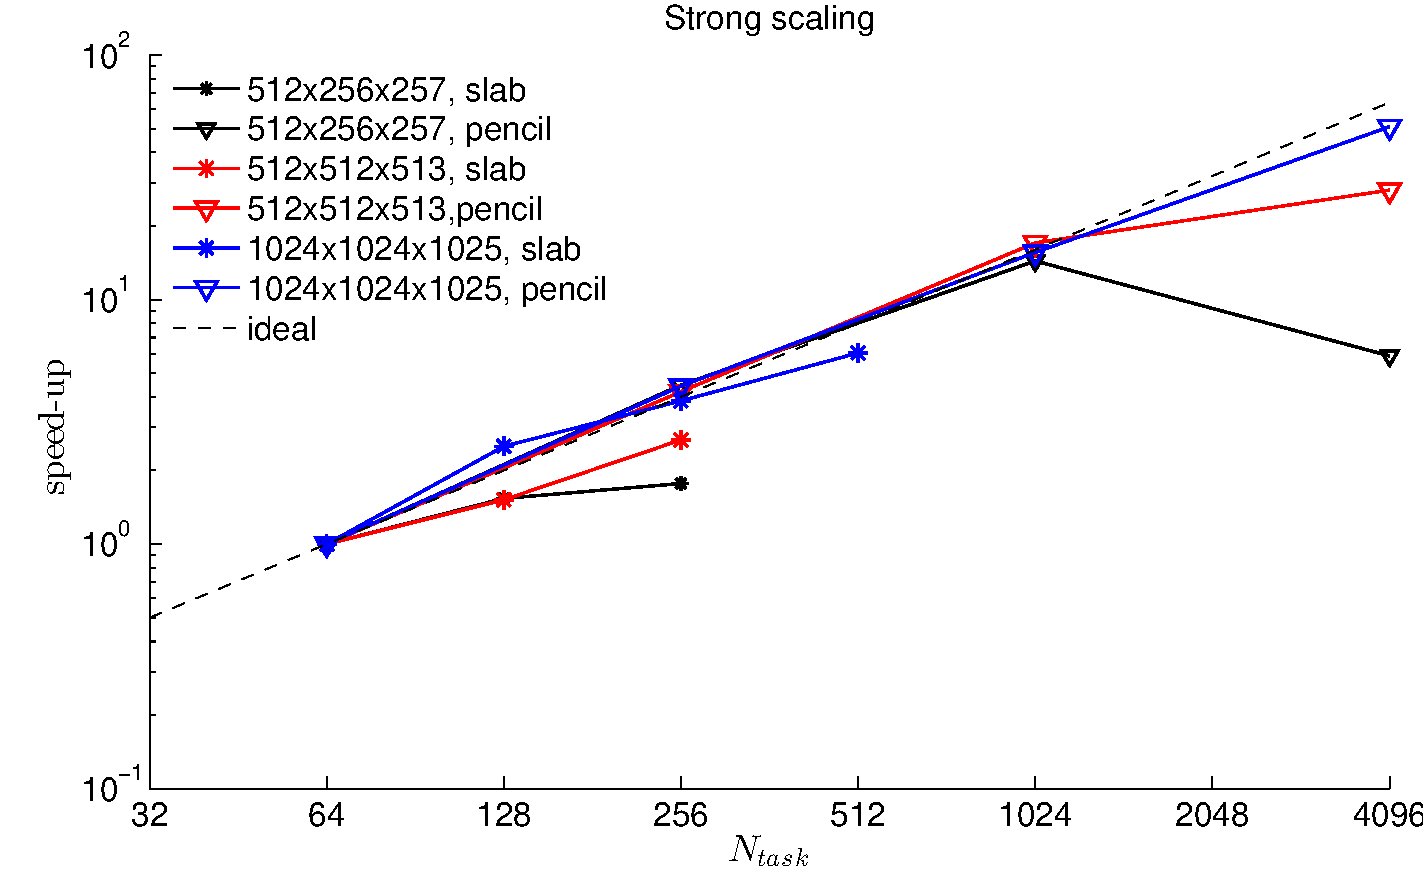
\includegraphics[width=0.9\textwidth]{strong_s_64}
\caption{Strong scalability}
\label{fig: strong_s}
\end{figure}
For the strong scalability case three different grids were tested both for slab and pencil domain decomposition: $512\times256\times257$, $512\times512\times513$ and $1024\times1024\times1025$. As commonly found in literature the speed-up obtained is normalized by the speed-up obtained on the lowest number of MPI processes used; in this case the lowest number was 64 MPI processes. The ideal behaviour is linear in the total number of MPI processes; as can be seen from Figure \ref{fig: strong_s} the slab decomposition runs deviate quite early from the ideal case, while the pencil cases keep an optimal speed-up at least up to 1\,024 MPI processes. At this point only the larger grid does not show worsening in the performance, while the smaller grids show a larger deviation from the ideal case. Due to the limit on the maximum number of cores  that can be requested on the Marconi A1 partition (around 6\,000), we could not verify the scalability on a higher number of MPI processes.\\
\begin{table}[H]
\centering
\caption{Strong scaling speed-up calculated with respect to 64 MPI processes case}
\begin{tabular}{c|c|c|c|c|c}
$N_{y,cpu}$ & $N_{z,cpu}$ & grid & time per time step [s] & speed-up &ideal speed-up\\[1.5ex]
1 & 64 & $512\times256\times257$&1.22 & 1& 1\\
1 & 128 & $512\times256\times257$& 0.79 &1.54& 2\\
1 &256& $512\times256\times257$& 0.69 & 1.77 &4\\
\hline
8& 8& $512\times256\times257$& 1.44  & 1 &1\\
16& 16 & $512\times256\times257$& 0.32 & 4.5& 4 \\
32 &32 & $512\times256\times257$& 0.10 & 14.4 &16 \\
64 &64 & $512\times256\times257$& 0.25 & 5.76 &64\\
\hline\hline
1& 64 & $512\times512\times513$& 4.82  & 1 &1\\
1& 128& $512\times512\times513$& 3.18  & 1.52 &2 \\
1 &256& $512\times512\times513$& 1.81 & 2.66 &4\\
\hline
8& 8 & $512\times512\times513$& 6.64 &  1 &1\\
16& 16 & $512\times512\times513$&1.58 & 4.20 &4\\
32 &32 & $512\times512\times513$&0.39& 17.03 &16\\
64 &64 & $512\times512\times513$&0.24 &  27.67 &64\\
\hline\hline
1& 64 & $1024\times1024\times1025$& 55.72 &1  &1 \\
1& 128& $1024\times1024\times1025$& 22.20 & 2.51 &2\\
1 &256& $1024\times1024\times1025$& 14.46 &3.85 &4\\
1 &512 & $1024\times1024\times1025$&9.20 & 6.06 &8\\
\hline
8& 8 & $1024\times1024\times1025$&62.40 & 1 &1\\
16& 16& $1024\times1024\times1025$& 14.10 & 4.43 &4\\
32 &32& $1024\times1024\times1025$& 4.00 &  15.6 &16\\
64 &64& $1024\times1024\times1025$& 1.23 & 50.73  &64\\
\end{tabular}
\end{table}
\begin{figure}[h!]
\centering
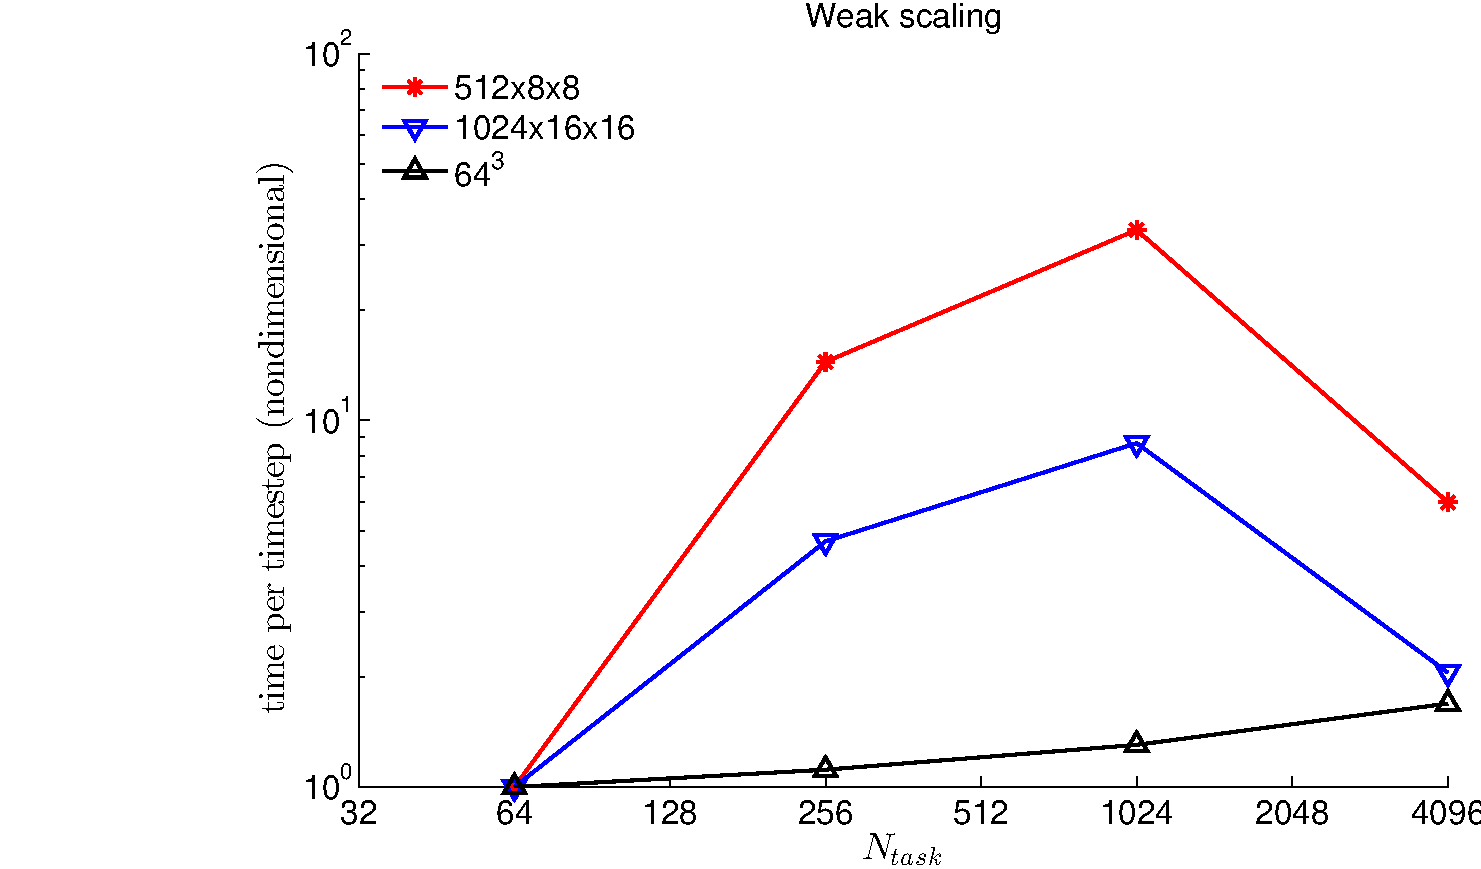
\includegraphics[width=0.9\textwidth]{weak_s_64}
\caption{Weak scalability}
\end{figure}
For the weak scalability case three different runs were run: in the first two cases denoted by $512\times8\times8$ and $1024\times16\times16$ the aspect ratio of the arrays was kept constant as the number of MPI processes increased. In the other case, denoted by $64^3$ only the total number of points per MPI process was kept constant. This allowed for a better data layout in memory, which gave much better results, only matched by the others two cases when the global grid approached a unitary aspect ratio in the three dimensions.
\begin{table}[H]
\centering
\caption{Weak scaling time per time step normalized with respect to 64 MPI processes case}
\begin{tabular}{c|c|c|c|c|c}
$N_{y,cpu}$ & $N_{z,cpu}$& load/core & grid & $t/t_{\textnormal{step}}$ [s] &$t/t_{\textnormal{step}}$ normalized\\[1.5ex]
8& 8 & $512\times8\times8$  &$512\times64\times65$ &  0.06 & 1\\
16 &16&$512\times8\times8$  & $512\times128\times129$& 0.81 & 14.46\\
32 &32&$512\times8\times8$  & $512\times256\times257$& 1.85 & 33.04\\
64 &64 &$512\times8\times8$  &$512\times512\times513$ & 0.34 & 6.07 \\
\hline
8& 8&$1024\times16\times16$  & $1024\times128\times129$ &0.54 &1 \\
16& 16& $1024\times16\times16$  & $1024\times256\times257$ &2.50 & 4.66\\
32 &32 &$1024\times16\times16$  & $1024\times512\times513$ &4.64 & 8.66\\
64 &64 &$1024\times16\times16$  & $1024\times1024\times1025$ &1.10 & 2.05\\
\hline
8& 8 & $64^3$& $256\times256\times257$ & 0.65& 1\\
16& 16&$64^3$&$512\times512\times257$ & 0.73 &1.12 \\
32& 32 &$64^3$&$512\times512\times1025$ &0.85 & 1.30 \\
64& 64 &$64^3$&$1024\times1024\times1025$ &1.10 &1.69 \\ 
\end{tabular}
\end{table}









%\chapter{Code validation}
\section{Single phase validation}
The code was validated running a simulation at $\Re_\tau=300$ starting from a fully developed turbulent channel flow; all the results were gathered on a timespan of 1\,500 $t^+$. The results were then compared with the DNS database of \cite{thtlab} at the same shear Reynolds number. Here is presented the outcome of this comparison; the data from \cite{thtlab} are denoted as tht-lab in the following pictures.\\
The velocity skewness was also compared with the old code results (\texttt{FlOWSB}), showing a perfect agreement.
\begin{figure}[H]
\centering
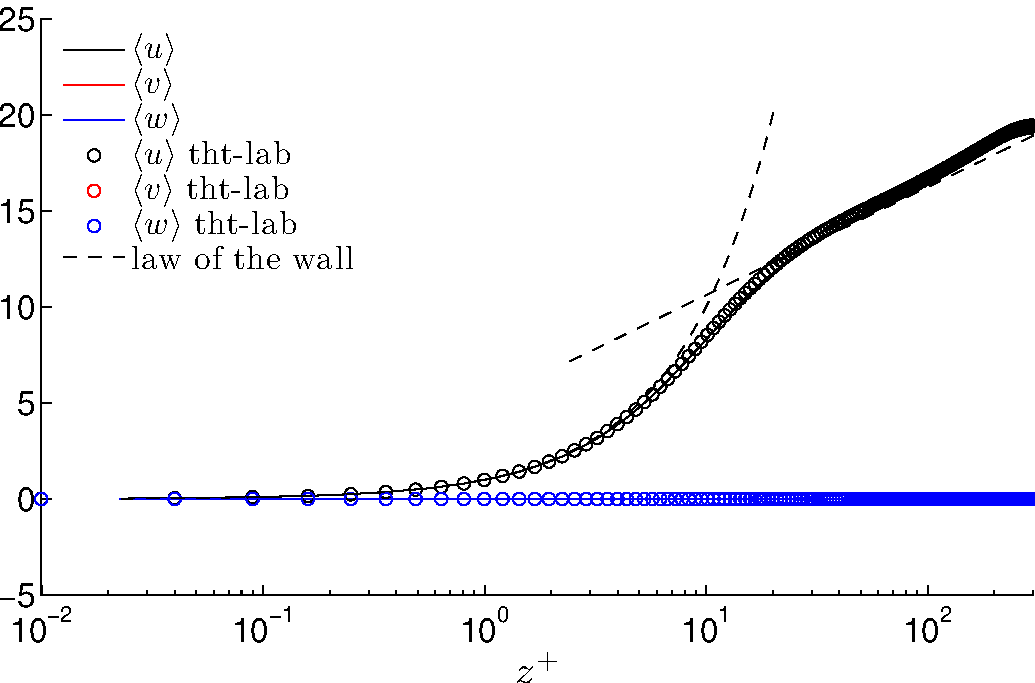
\includegraphics[width=\textwidth]{mean}
\caption{Mean velocity}
\end{figure}
\begin{figure}[H]
\centering
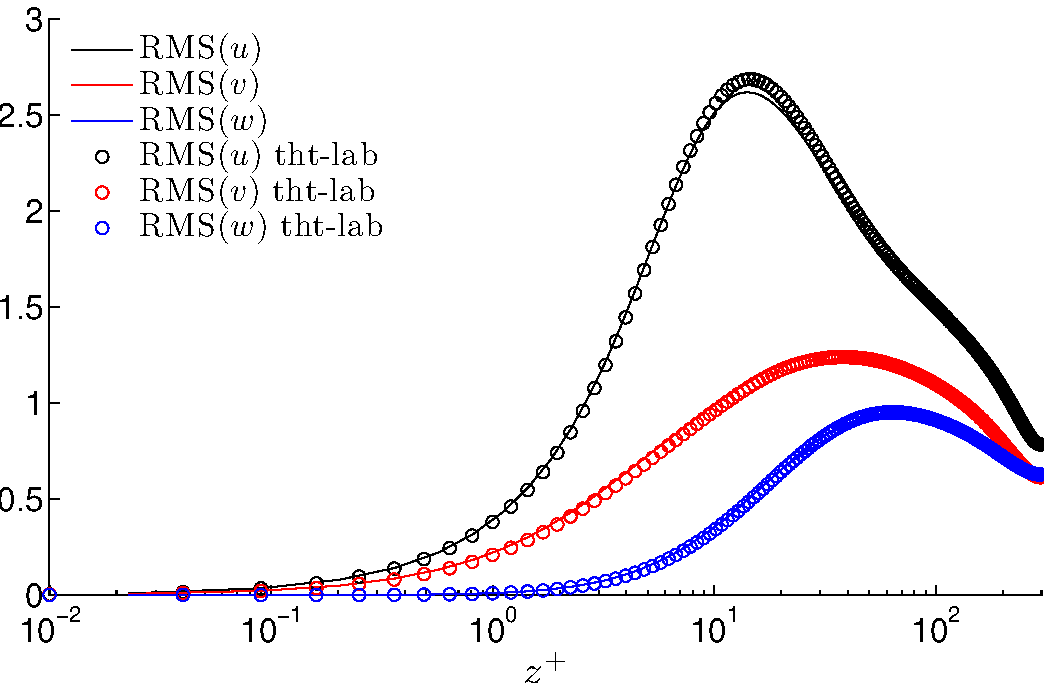
\includegraphics[width=\textwidth]{rms}
\caption{Velocity root mean square}
\end{figure}
\begin{figure}[H]
\centering
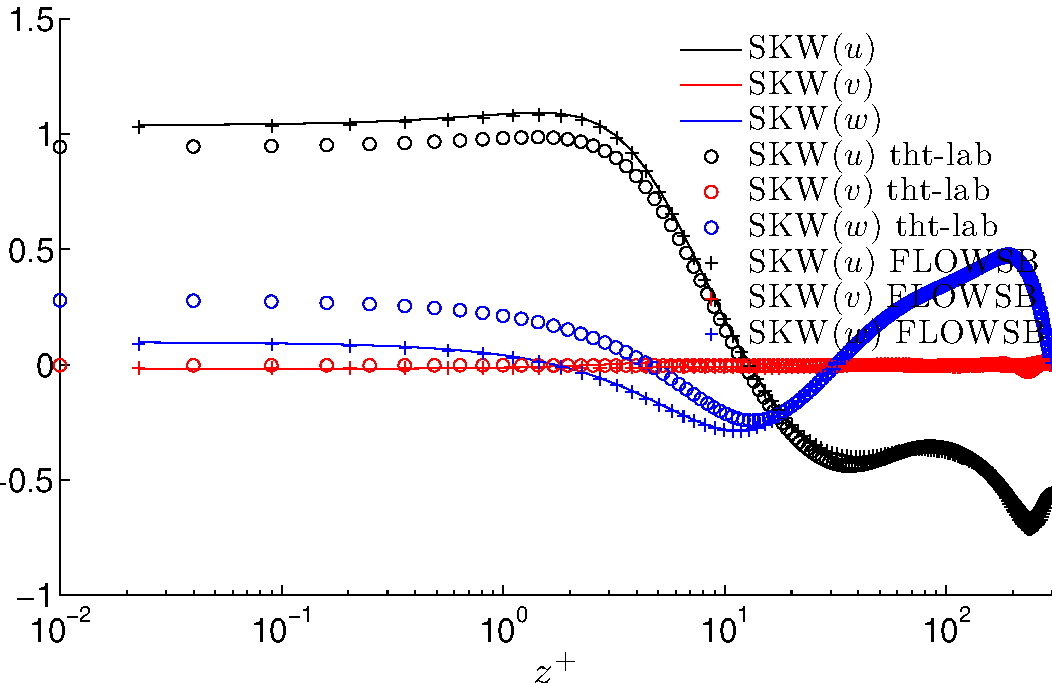
\includegraphics[width=\textwidth]{skw}
\caption{Velocity skewness}
\end{figure}
\begin{figure}[H]
\centering
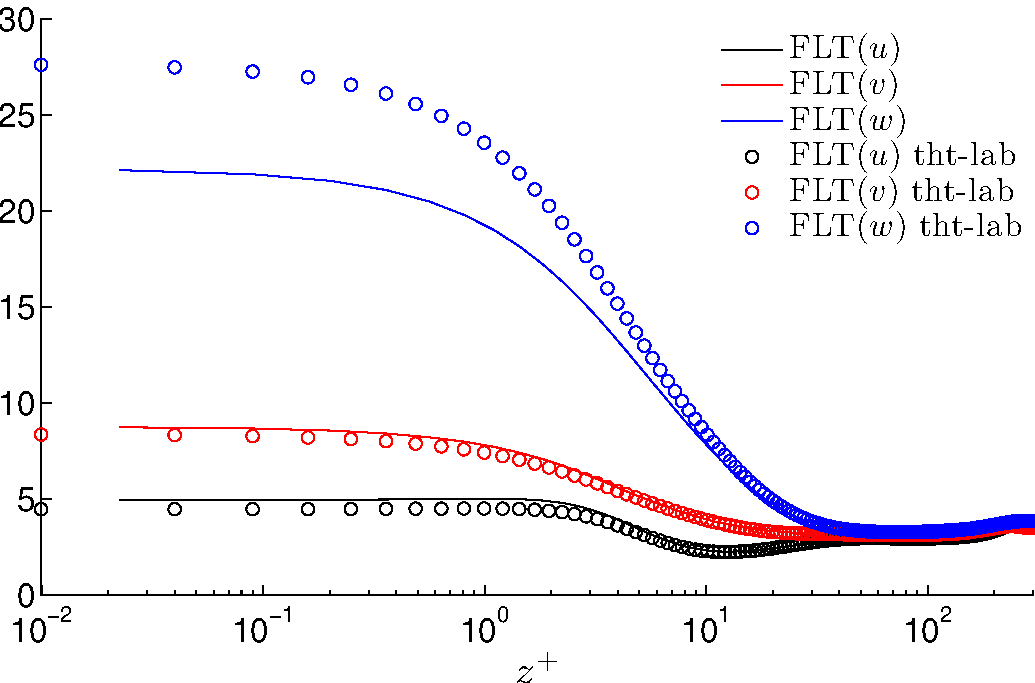
\includegraphics[width=\textwidth]{flt}
\caption{Velocity flatness}
\end{figure}
\begin{figure}[H]
\centering
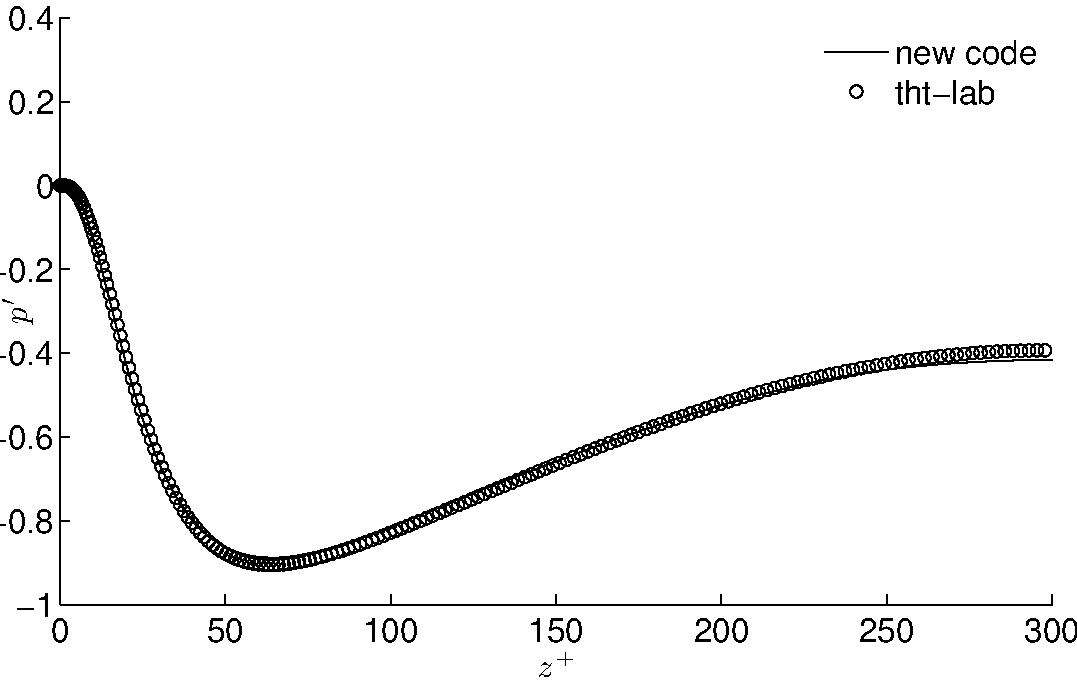
\includegraphics[width=\textwidth]{pmean}
\caption{Mean pressure}
\end{figure}
\begin{figure}[H]
\centering
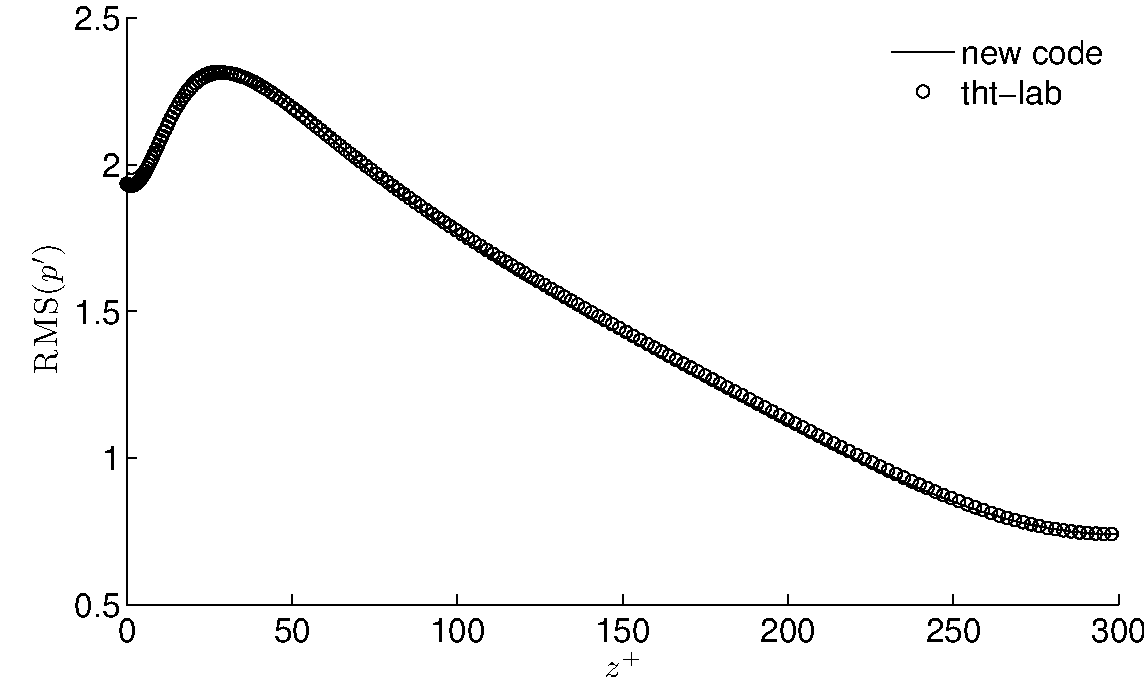
\includegraphics[width=\textwidth]{prms}
\caption{Pressure root mean square}
\end{figure}
\begin{sidewaysfigure}
\centering
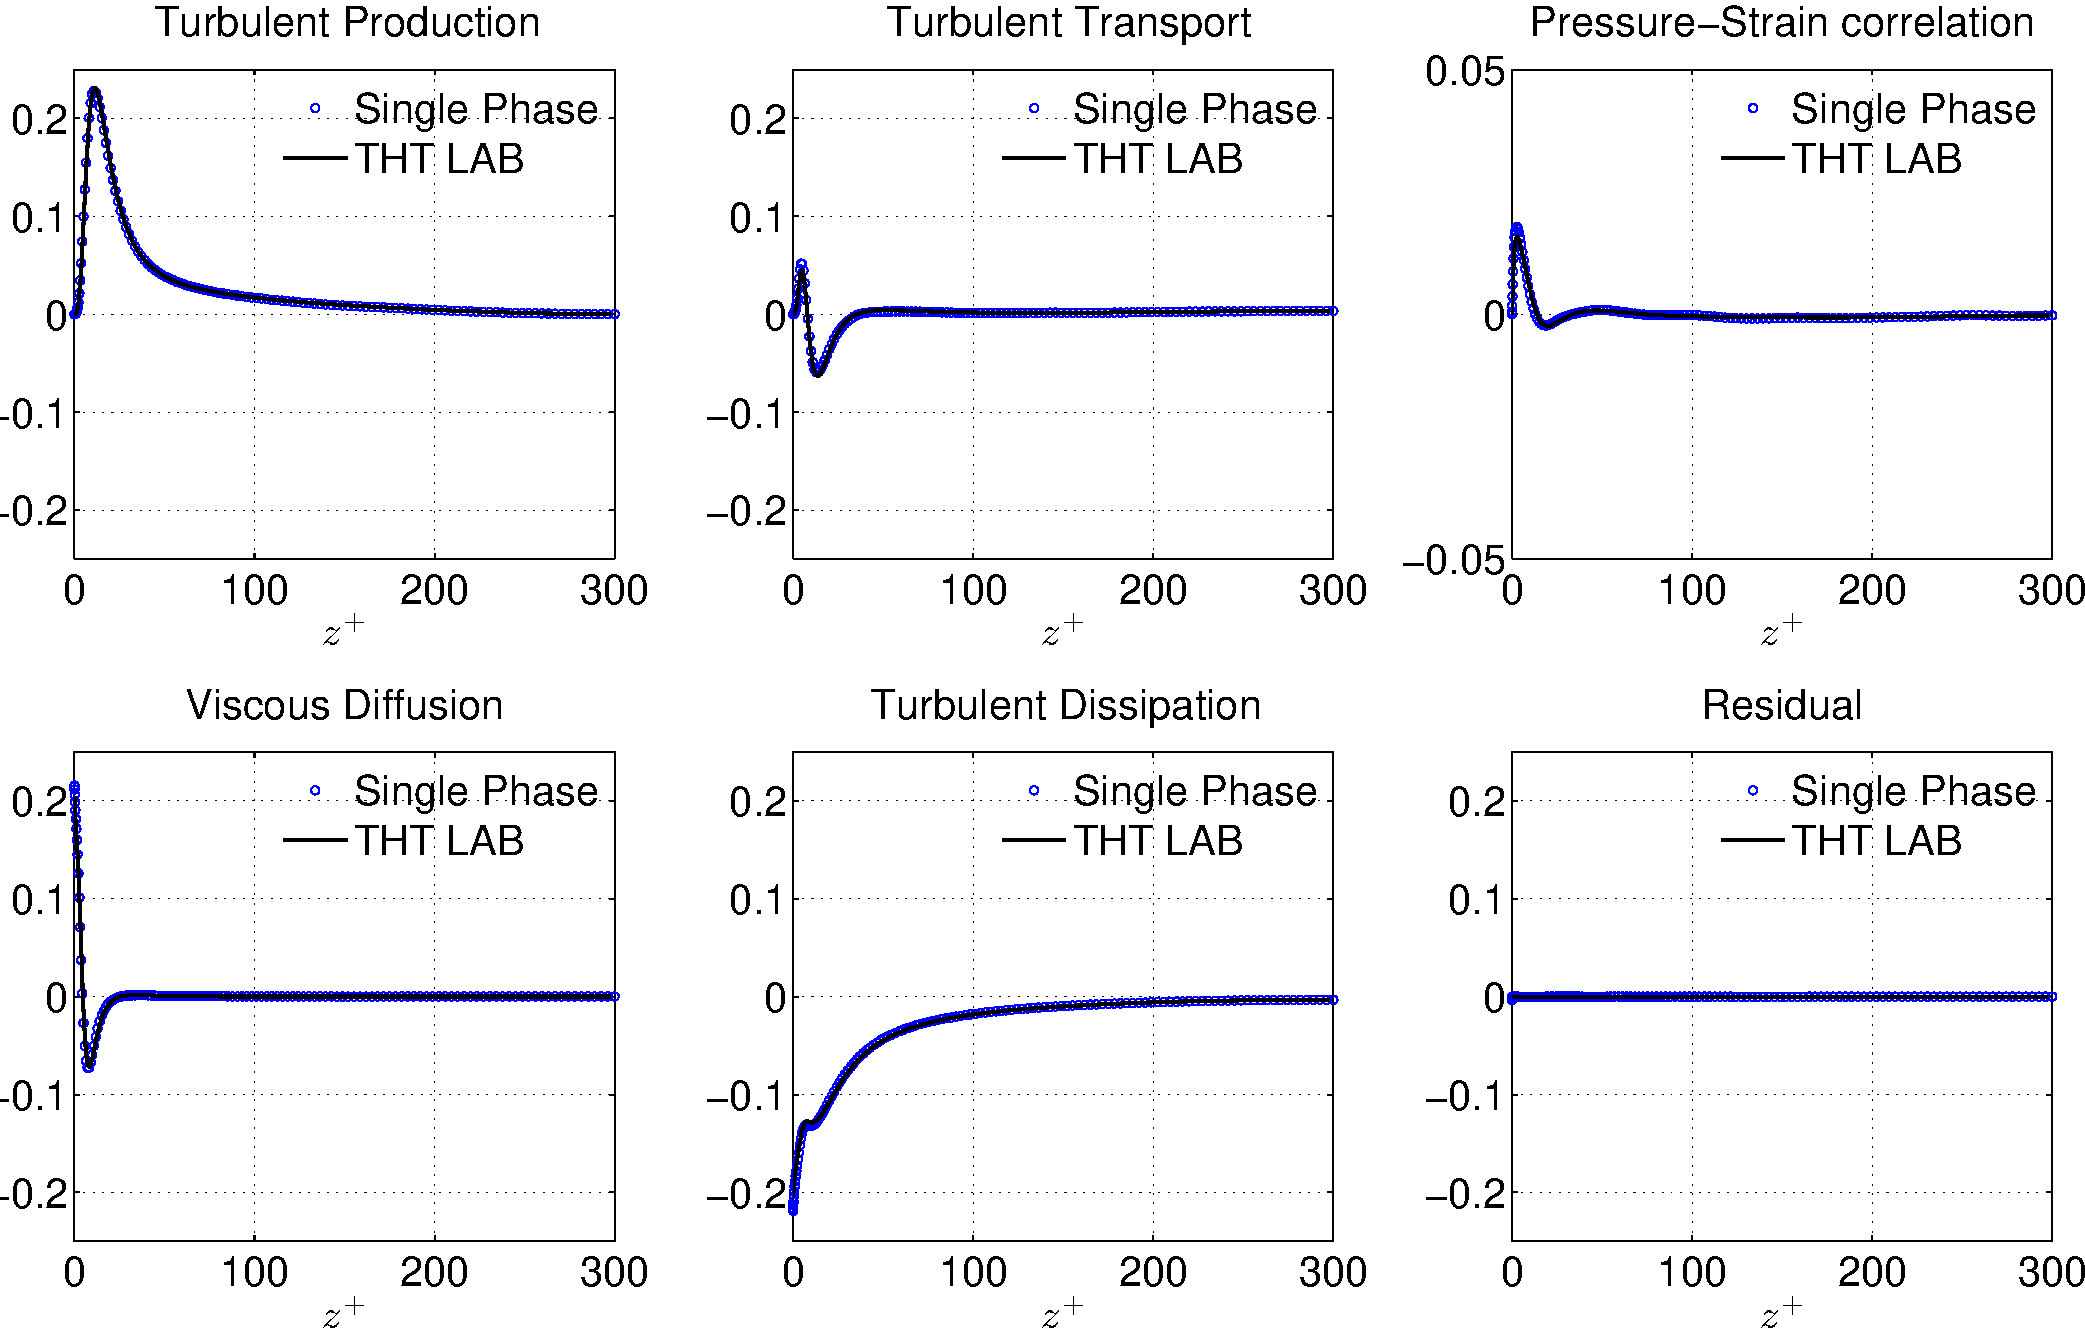
\includegraphics[width=\textwidth]{budget}
\caption{Energy budget}
\end{sidewaysfigure}
\begin{sidewaysfigure}
\centering
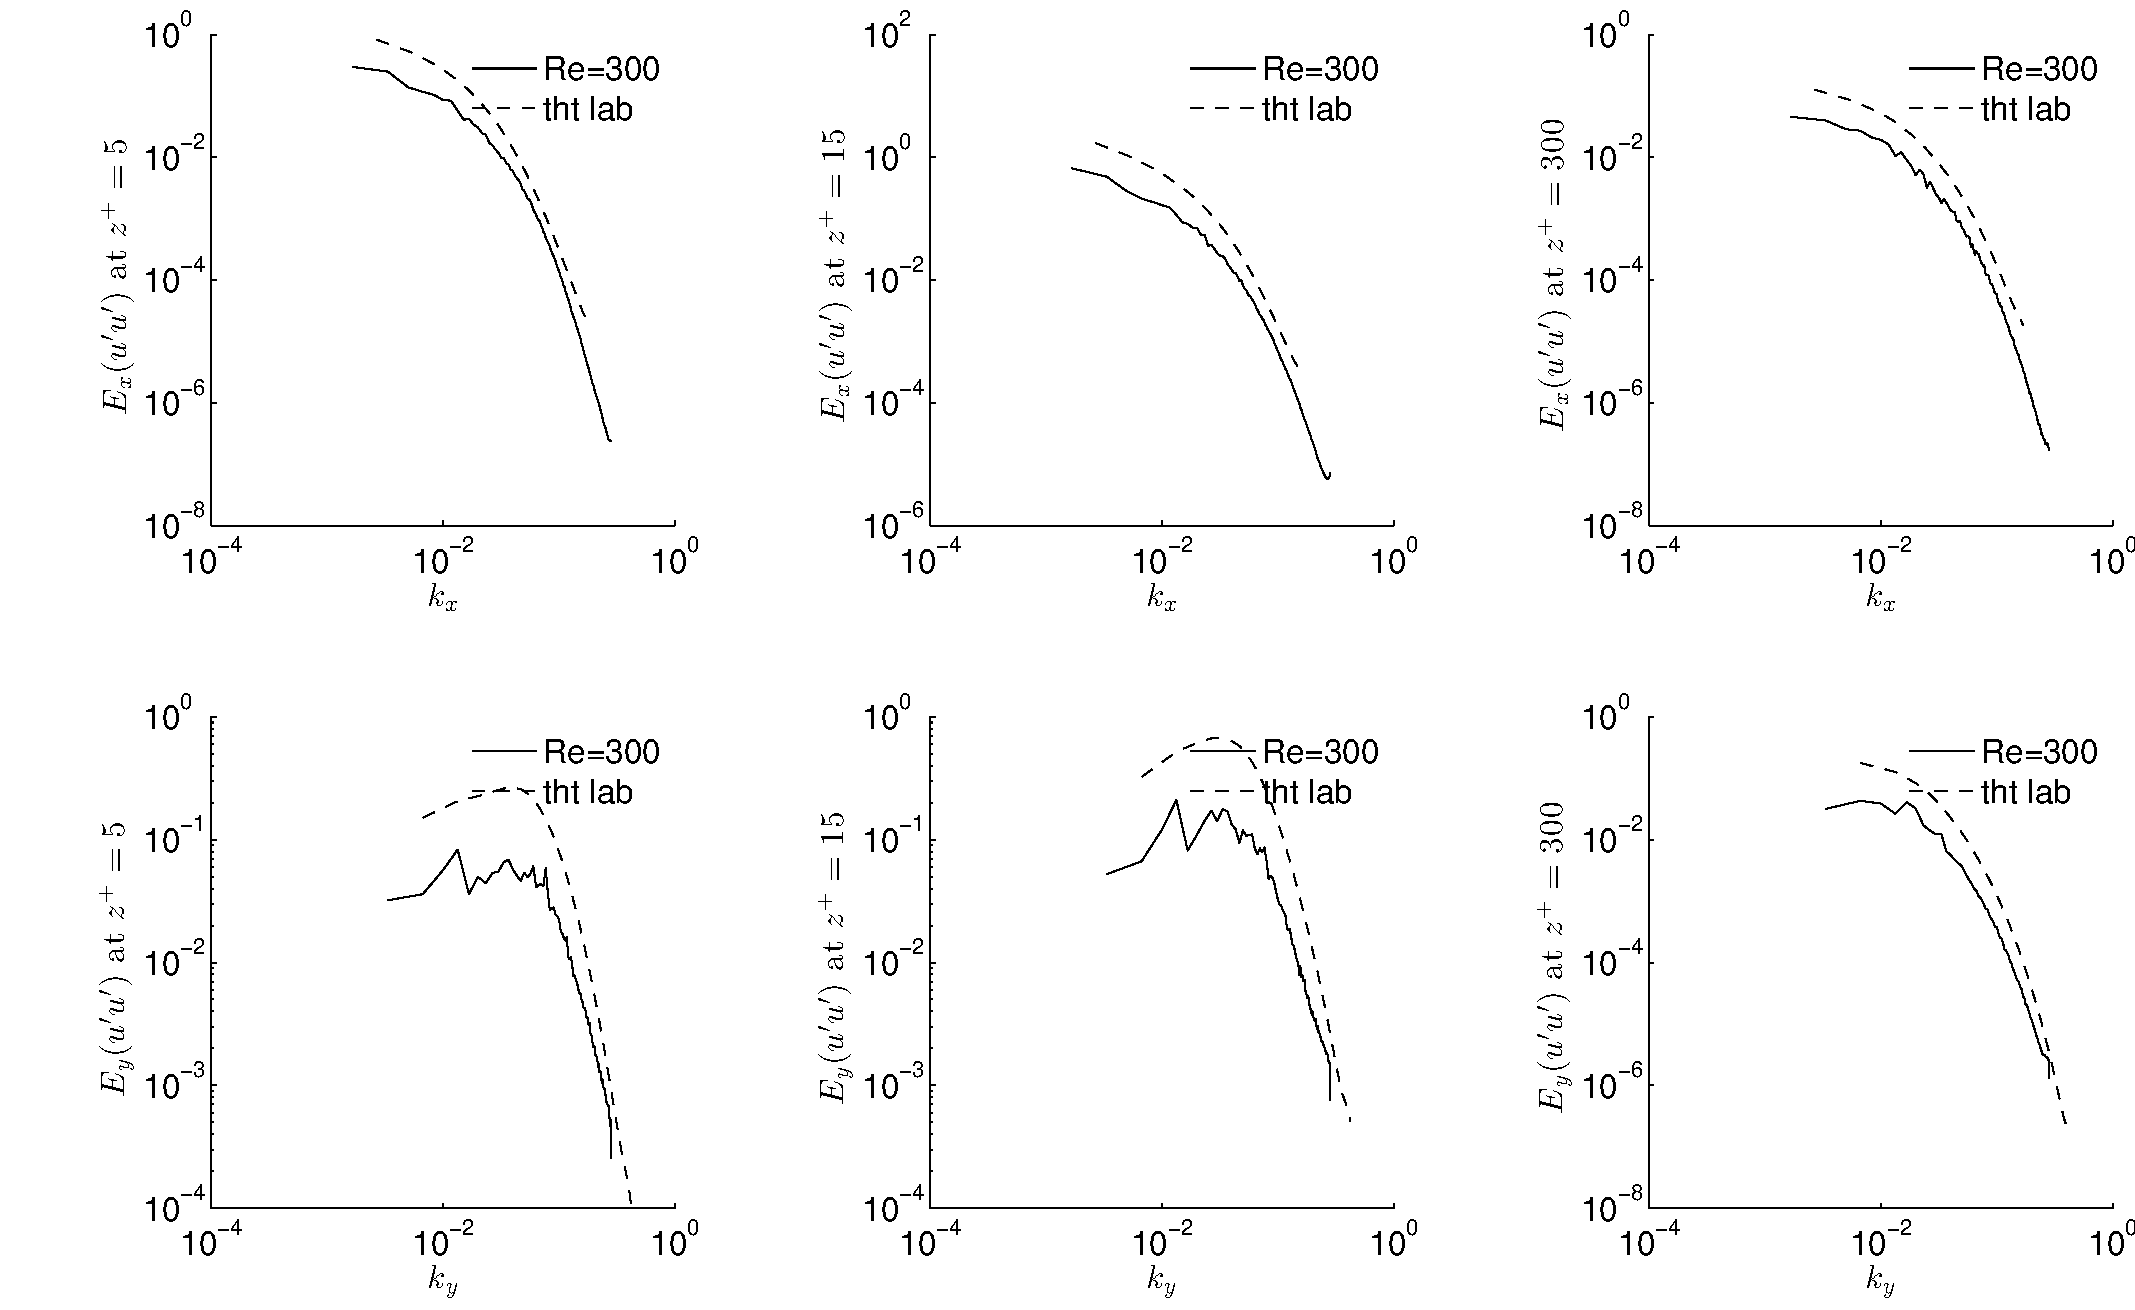
\includegraphics[width=\textwidth]{u_spectra}
\caption{$u'$ power spectra}
\end{sidewaysfigure}
\begin{sidewaysfigure}
\centering
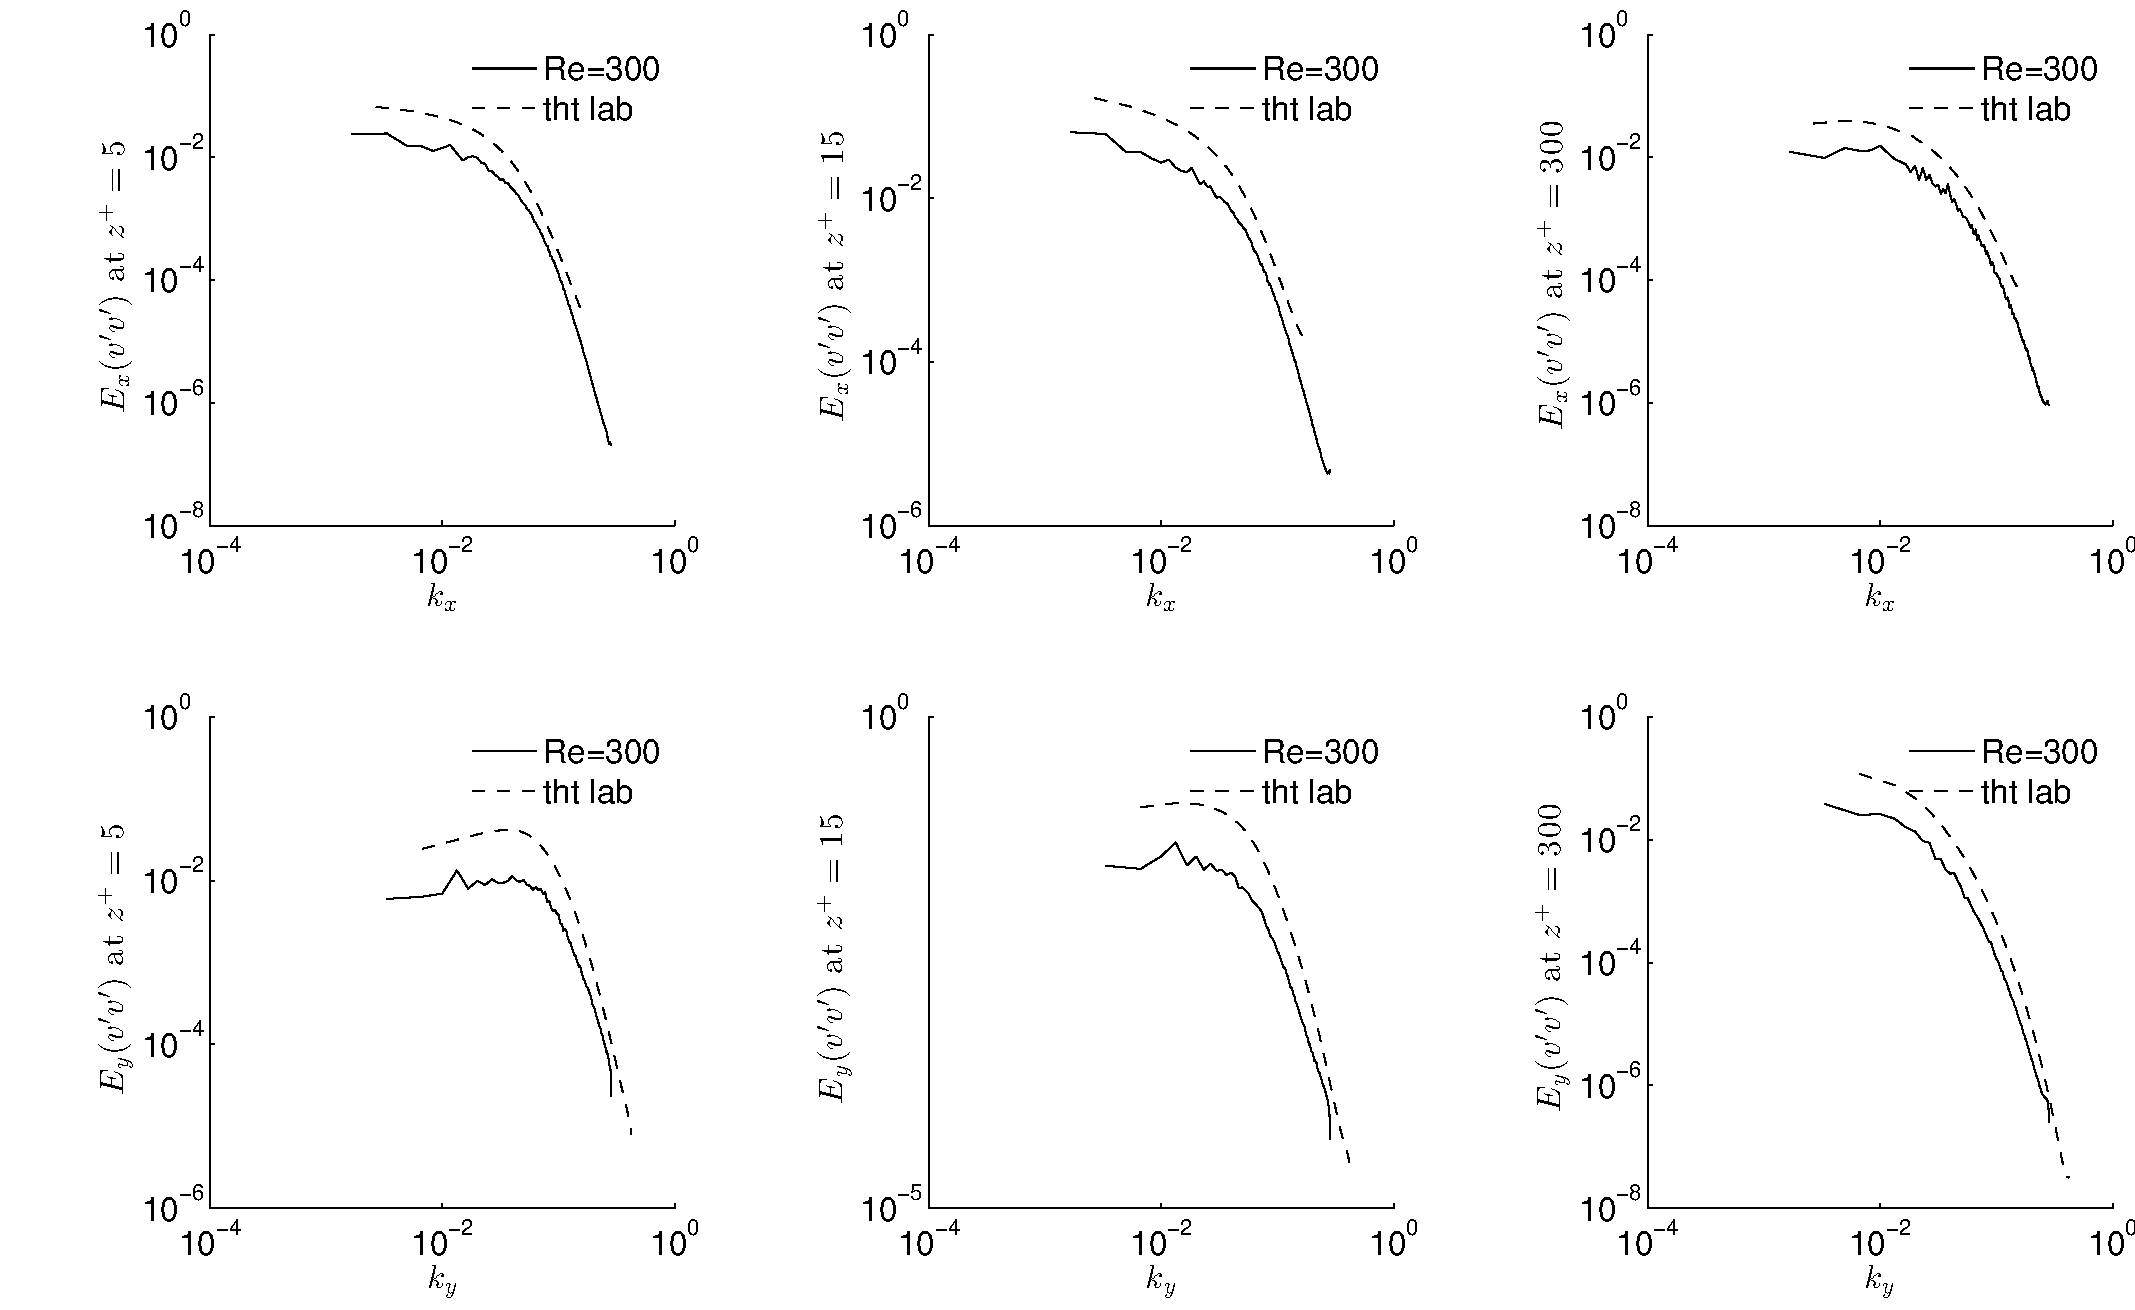
\includegraphics[width=\textwidth]{v_spectra}
\caption{$v'$ power spectra}
\end{sidewaysfigure}
\begin{sidewaysfigure}
\centering
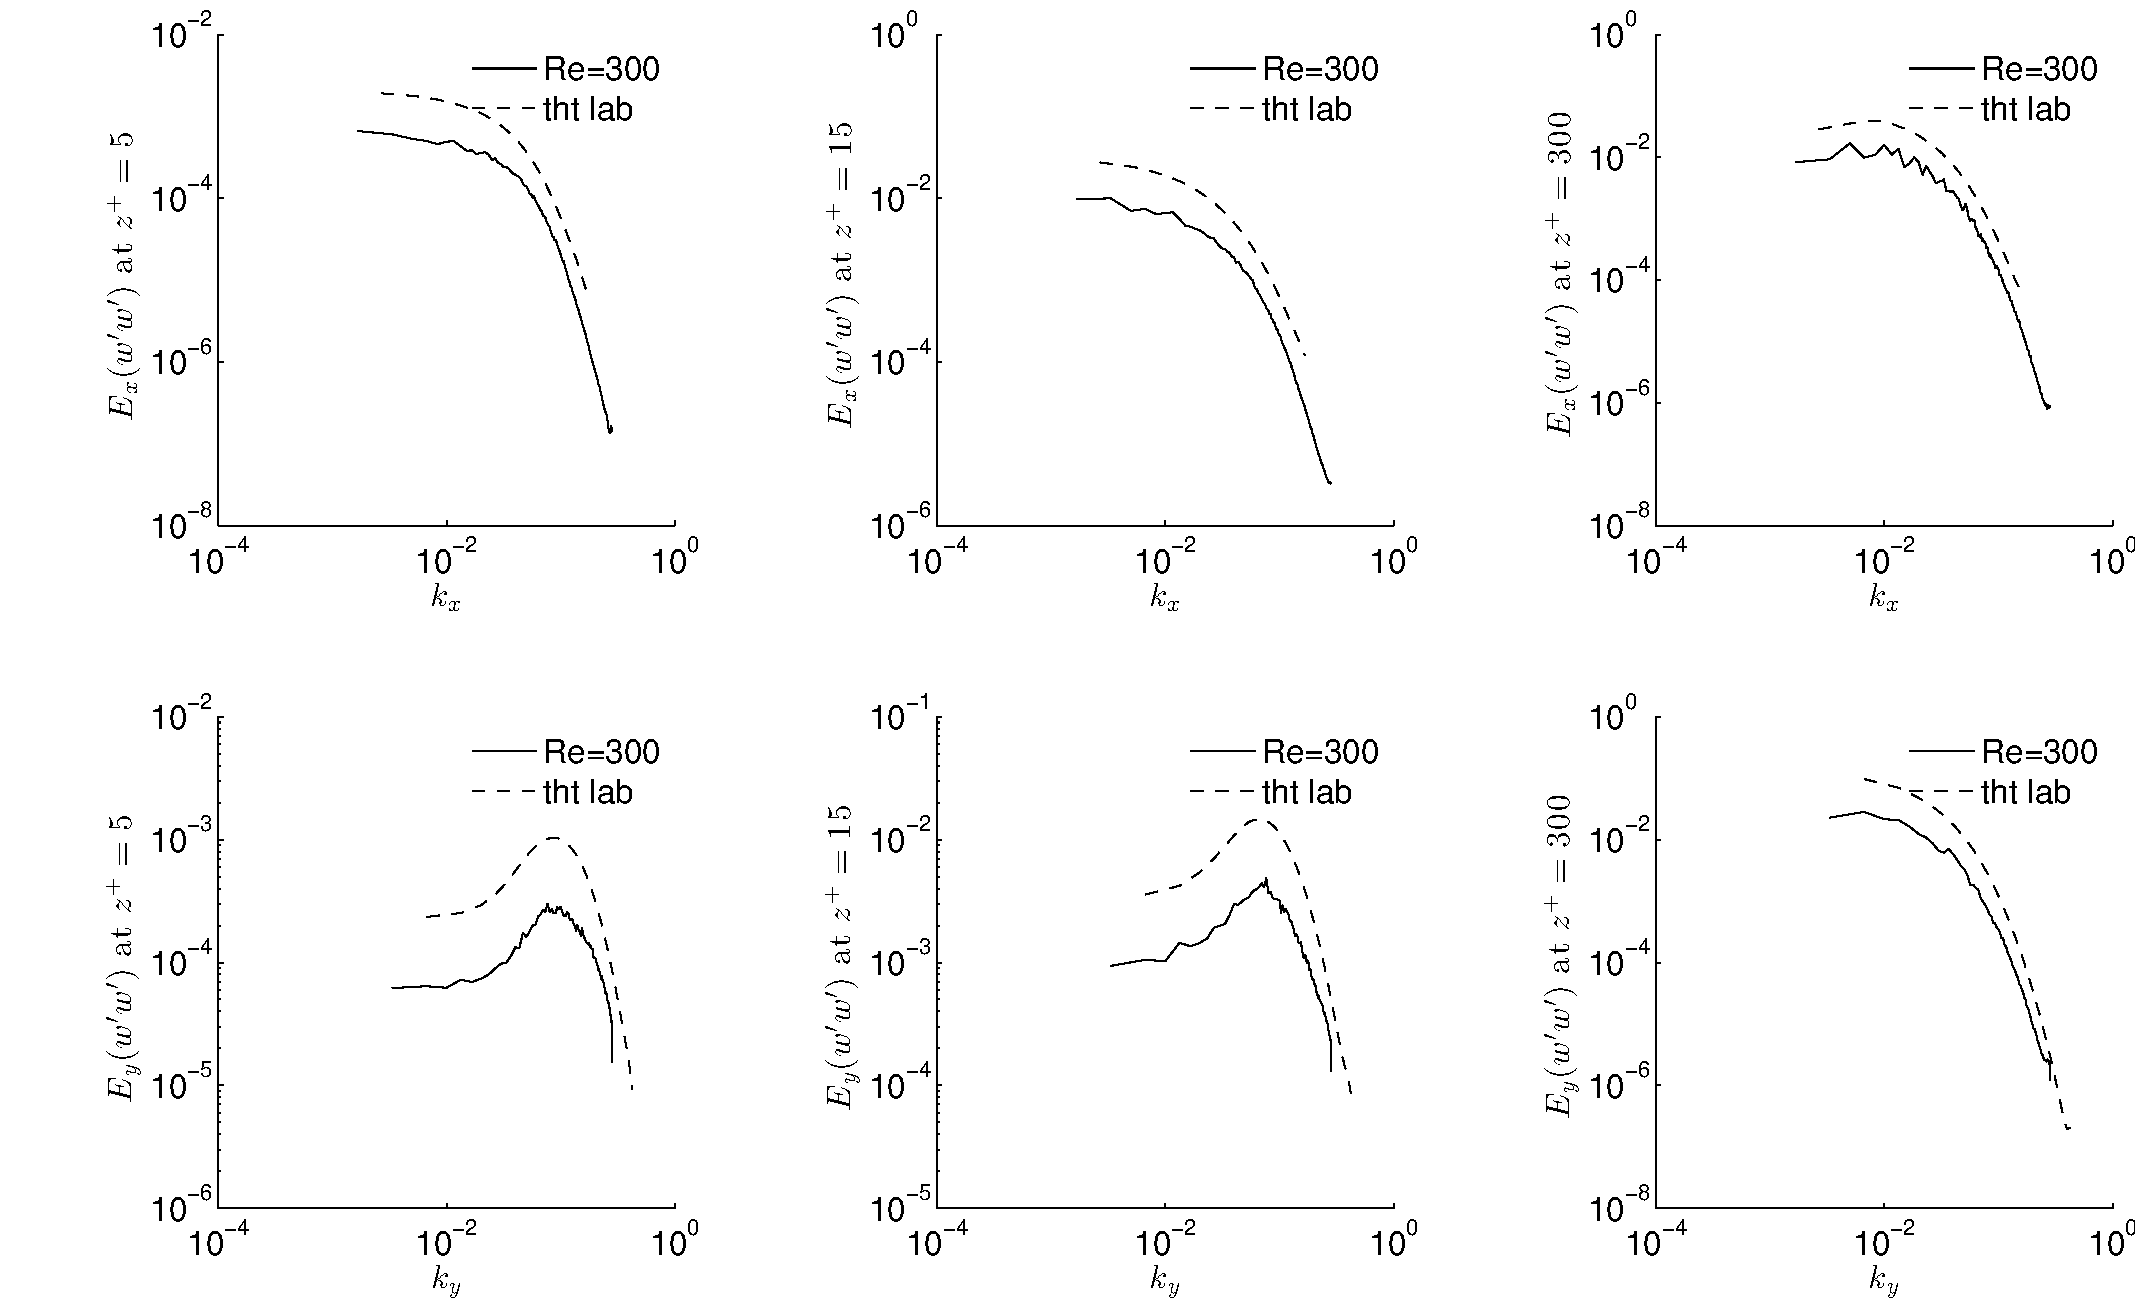
\includegraphics[width=\textwidth]{w_spectra}
\caption{$w'$ power spectra}
\end{sidewaysfigure}


\newpage
\section{Phase field validation}
The phase field was validated using the undamped analytical solution from \cite{Prosperetti81} for capillary waves at the interface between two superposed fluids (stable configuration). 
\begin{figure}[H]
\centering
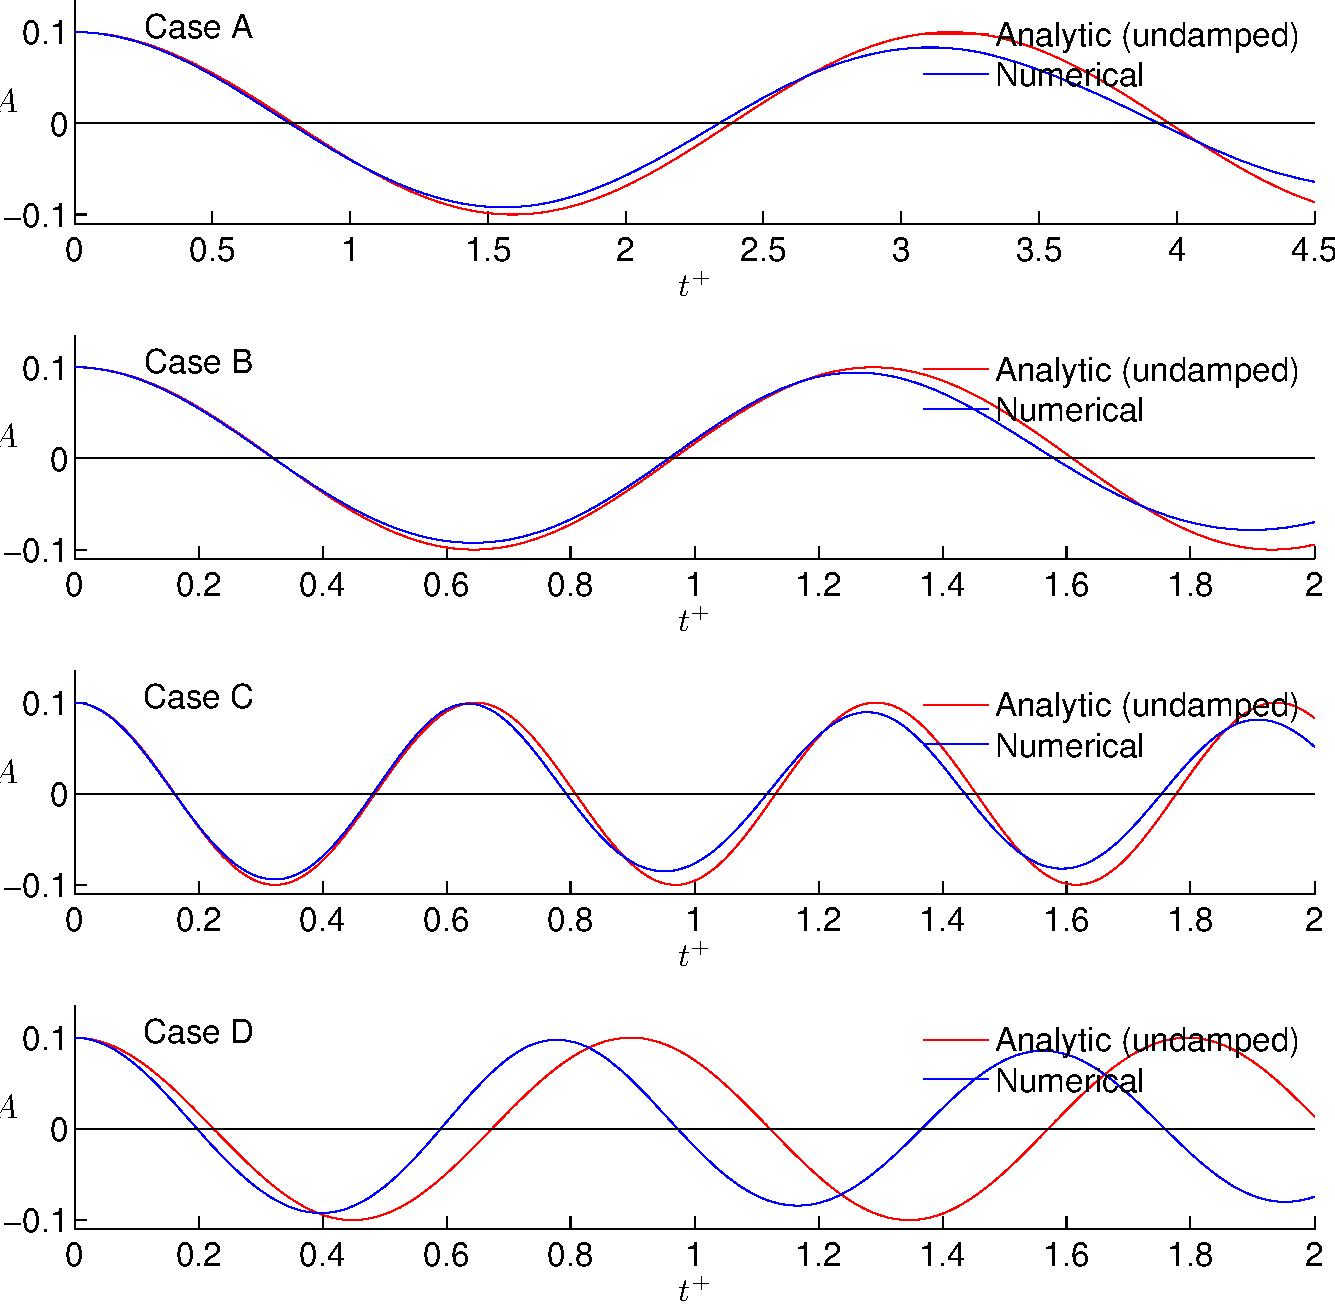
\includegraphics[width=\textwidth]{cap_waves}
\caption{Capillary waves, comparison of numerical solution (damped) with Prosperetti analytic solution (undamped). \textbf{Case A} : $\rho_R=0.9$, $\Fr=0.1$, $k_y=1$. \textbf{Case B} : $\rho_R=0.5$, $\Fr=0.1$, $k_y=1$. \textbf{Case C} : $\rho_R=0.5$, $\Fr=0.05$, $k_y=1$. \textbf{Case D} : $\rho_R=0.5$, $\Fr=0.1$, $k_y=2$.}
\end{figure}

\begin{table}[H]
\centering
\caption{Case run for phase field validation}
\begin{tabular}{l|c|c|c|c|c}
Case  & $\omega_0$ (analytic) & $\omega$ (numerical) & $\Delta \omega=\frac{\omega_0-\omega}{\omega_0}\cdot100$ [\%] & Density ratio & $\Fr$ \\[0.5ex]
\hline
Case A &1.976789 & 1.993080& -0.82  &0.9&0.1\\[0.5ex]
Case B &4.879132 &4.986655  & -2.20&0.5&0.1\\[0.5ex]
Case C & 9.721965& 9.933890&   -2.18&0.5&0.05\\[0.5ex]
Case D &7.001862 & 8.107336 &-15.79 &0.5& 0.1\\[0.5ex]
\end{tabular}
\end{table}






% references
\nocite{*}
\bibliographystyle{plainnat}
\bibliography{cap/biblio}
\clearpage{\pagestyle{empty}\cleardoublepage}

\listoffigures
\listoftables

\end{document}